\documentclass[10pt, a4paper]{report}
\usepackage{preamble/trymtex}
\usepackage{optidef}
\usepackage[acronym,symbols,nogroupskip]{glossaries-extra}
\usepackage[backend=biber]{biblatex}
\usepackage{forest}
\usetikzlibrary{
    backgrounds,
    positioning,
    arrows.meta,
    calc,
    decorations.pathreplacing,
    3d
}
\usetikzlibrary{arrows.meta}

\makeglossaries
\addbibresource{preamble/bib/references.bib}
\setglossarystyle{listhypergroup}

\includeonly{
     preamble/frontmatter/titlepage,
     preamble/bib/glossary,
%     chapters/1/introduction,
%     % chapters/2/unconstrained_optimization,
        chapters/3/constrained_optimization,
%     % preamble/appendix/AlgorithmMap,
%     % preamble/appendix/Formulas,
%     % preamble/appendix/Functions,
%     preamble/appendix/LectureNotes,
}

\begin{document}
% ===================================================
% Glossary
% ===================================================
\newglossaryentry{hessian}
{
    name=Hessian-matrise,
    description={En kvadratisk matrise av andre partielle deriverte av en funksjon med flere variabler, som beskriver lokal krumning av funksjonen.},
    symbol={$\nabla^2 f(x)$ eller $H(x)$}
}

\newglossaryentry{feasible-region}
{
    name=tillatt område,
    description={Mengden av alle mulige punkter som tilfredsstiller alle bibetingelser i et optimeringsproblem.},
    symbol={$\mathcal{X}$}
}

\newglossaryentry{convex-function}
{
    name=konveks funksjon,
    description={En funksjon $f$ der linjesegmentet mellom to vilkårlige punkter på funksjonen aldri ligger under funksjonsgrafen. Matematisk: $f(\lambda x + (1-\lambda)y) \leq \lambda f(x) + (1-\lambda)f(y)$ for alle $x, y$ og $\lambda \in [0,1]$.},
    symbol={$f$ er konveks}
}

\newglossaryentry{local-minimum}
{
    name=lokalt minimum,
    description={Et punkt $x^*$ hvor funksjonsverdien er mindre enn eller lik verdiene i en liten omegn rundt punktet. Formelt: Det eksisterer en $\delta > 0$ slik at $f(x^*) \leq f(x)$ for alle $x$ med $\|x - x^*\| < \delta$.},
    symbol={$x^*$ lokalt min}
}

\newglossaryentry{global-minimum}
{
    name=globalt minimum,
    description={Et punkt $x^*$ hvor funksjonsverdien er mindre enn eller lik verdien for alle andre punkter i definisjonsmengden. Formelt: $f(x^*) \leq f(x)$ for alle $x$ i definisjonsmengden.},
    symbol={$x^*$ globalt min}
}

\newglossaryentry{gradient}
{
    name=gradient,
    description={En vektor som gir retningen og størrelsen på den maksimale økningen av en funksjon i et gitt punkt. For en funksjon $f(x)$ er gradienten gitt ved $\nabla f(x) = (\frac{\partial f}{\partial x_1}, \frac{\partial f}{\partial x_2}, \ldots, \frac{\partial f}{\partial x_n})$.},
    symbol={$\nabla f(x)$}
}

\newglossaryentry{lagrange-multiplier}
{
    name=lagrange-multiplikator,
    description={En variabel brukt i lagrange-metoden for å finne ekstremalpunkter til en funksjon underlagt bibetingelser. For et problem med mål $f(x)$ og bibetingelser $g(x) = 0$, danner vi Lagrange-funksjonen $L(x, \lambda) = f(x) - \lambda g(x)$.},
    symbol={$\lambda$}
}

\newglossaryentry{kkt-conditions}
{
    name=KKT-betingelser,
    description={Nødvendige første-ordens betingelser for at en løsning skal være optimal i et optimeringsproblem med bibetingelser, oppkalt etter Karush, Kuhn og Tucker. Inkluderer stasjonaritetsbetingelsen, komplementær slakk, primal og dual gjennomførbarhet.},
    symbol={$\nabla f(x^*) + \sum_{i=1}^m \lambda_i \nabla g_i(x^*) = 0$},
    see={first-order-necessary-conditions}
}
\newglossaryentry{slater-condition}{
    name=slakkbetingelse,
    description={En betingelse i KKT-betingelsene som sier at produktet av Lagrange-multiplikatoren og bibetingelsen må være null. Dette betyr at enten er multiplikatoren null eller så er bibetingelsen lik null.},
    symbol={$g_i(x) \geq 0$},
    see={kkt-conditions}
}

\newglossaryentry{first-order-necessary-conditions}{
    name={First-order necessary conditions},
    description={
        Betingelser som må være oppfylt for at en løsning skal være optimal i et optimeringsproblem. Disse inkluderer gradienten av målfunksjonen og bibetingelsene.
    },
    symbol={$\nabla f(x^*) = 0$}
    see={kkt-conditions},
}

\newglossaryentry{steepest-descent}{
    name={Steepest Descent},
    description={
        En metode for å finne minimum av en funksjon ved å følge den bratteste nedstigningen i gradienten \(d_k = -\nabla f(x_k)\). Dette innebærer å ta et skritt i retning av den negative gradienten for å minimere funksjonen.
    },
    symbol={$d_k = -\nabla f(x_k)$},
    see={gradient},
}




% ==================================================
% Acronyms
% ==================================================
\newacronym{kkt}{KKT}{Karush-Kuhn-Tucker betingelser}

\newacronym{gd}{GD}{Gradient Descent}

\newacronym{ls}{LS}{Line Search}

\newacronym{lp}{LP}{Lineær Programmering}

\newacronym{nlp}{NLP}{Ikke-lineær Programmering}

\newacronym{qp}{QP}{Kvadratisk Programmering}


\begin{titlepage}
    \newcommand{\HRule}{\rule{\linewidth}{0.5mm}}
    \center
    
    % Top section with logo
    \vspace*{2cm}
    \begin{center}
        
\includegraphics[width=5cm]{preamble/frontmatter/TS_GooseLogo.png}
    \end{center}
    
    \vspace{2cm}
    
    % Course code & title with modern styling
    {\color{ntnu-blue}\sffamily\LARGE TMA4180 \par}
    \vspace{0.8cm}
    {\sffamily\huge\bfseries\color{black} Optimering I \par}
    
    \vspace{1.5cm}
    
    % Stylized separator
    {\color{ntnu-lightblue}\HRule}
    \vspace{0.75cm}
    {\Large\sffamily\color{ntnu-blue} Notater i Optimering I \par}
    \vspace{0.75cm}
    {\color{ntnu-lightblue}\HRule}
    
    \vspace{2cm}
    
    % Author and semester info with modern layout
    \begin{minipage}{0.48\textwidth}
        \begin{flushleft}
            \large
            {\color{ntnu-blue}\textbf{Author}}\par
            \vspace{0.2cm}
            Trym Sæther\par
            \vspace{0.3cm}
            
\includegraphics[height=1cm]{preamble/frontmatter/TS_Signature.png}\par
            \vspace{0.3cm}
            {\color{ntnu-purple}\textit{Physics and Mathematics}}
        \end{flushleft}
    \end{minipage}
    \hfill
    \begin{minipage}{0.48\textwidth}
        \begin{flushright}
            \large
            {\color{ntnu-blue}\textbf{Semester}}\par
            \vspace{0.2cm}
            Spring 2025\par
            6th semester
        \end{flushright}
    \end{minipage}
    
    \vfill
    
    % University info with modern styling
    \begin{center}
        {\color{ntnu-blue}\sffamily\Large Norwegian University of Science and Technology}
        \vspace{0.4cm}
        
        {\sffamily\large Department of Mathematical Sciences}
    \end{center}
    
    \vspace{1cm}
\end{titlepage}

\tableofcontents

\clearpage

\part{Optimeringsproblemer og Optimalitet}
\label{part:introduction}

\chapter{Matematisk bakgrunn}
\label{chap:mathematical_background}

\section{Grunnleggende lineær algebra}
\subsection{Vektor operasjoner}

\subsubsection{Indre produkt}
Det indre produktet, også kjent som skalarprodukt, er en operasjon som tar to vektorer og gir et tall. 
Dette tallet representerer på mange måter hvordan vektorene "overlapper" med hverandre, og er spesielt nyttig for å måle avstander og vinkler mellom vektorer.

\begin{definition}{Indre produkt}{inner_product}
	Gitt to vektorer \( \symbf{u}, \symbf{v} \in \R^n \), er det indre produktet definert som:

	\[
		\symbf{u} \cdot \symbf{v} = \symbf{u}^\top \symbf{v} = \sum_{i=1}^{n} u_i v_i
	\]

\end{definition}

\begin{remark}{Projeksjon}{projection}
	Projeksjonen av vektoren \( \symbf{u} \) på vektoren \( \symbf{v} \) er gitt ved:
	\[
		\operatorname{proj}_{\symbf{v}}(\symbf{u}) = \frac{\symbf{u} \cdot \symbf{v}}{\norm{\symbf{v}}^2} \symbf{v}
	\]
	Dette gir oss en ny vektor som er parallell med \( \symbf{v} \) og representerer den delen av \( \symbf{u} \) som "går i retning" av \( \symbf{v} \).
\end{remark}

\subsubsection{Ytre produkt (tensorprodukt)}
Ytre produktet er en operasjon som tar to vektorer og lager en matrise.
\begin{definition}{Ytre produkt}{outer_product}
	Gitt to vektorer \( \symbf{u} \in \R^m \) og \( \symbf{v} \in \R^n \), er det ytre produktet definert som:
	\[
		\symbf{u} \otimes \symbf{v} = \symbf{u} \; \symbf{v}^\top =
		\begin{bmatrix}
			u_1v_1 & u_1v_2 & \cdots & u_1v_n \\
			u_2v_1 & u_2v_2 & \cdots & u_2v_n \\
			\vdots & \vdots & \ddots & \vdots \\
			u_mv_1 & u_mv_2 & \cdots & u_mv_n
		\end{bmatrix}
	\]
\end{definition}

\subsubsection{Norm}
En norm er en funksjon som måler \enquote{størrelsen} eller \enquote{lengden} av matematiske objekter som vektorer. 
Den generaliserer ideen om absolutt verdi til høyere dimensjoner.

\begin{definition}{Norm}{norm}
	En norm på et vektorrom \(V\) er en funksjon \(\norm{\cdot}: V \to \R\) som oppfyller:
	\begin{enumerate}
		\item \textbf{Positivitet:} \(\norm{\symbf{x}} \geq 0\) og \(\norm{\symbf{x}} = 0\) hvis og bare hvis \(\symbf{x} = 0\)
		\item \textbf{Homogenitet:} \(\norm{\alpha \symbf{x}} = |\alpha| \norm{\symbf{x}}\) for alle \(\alpha \in \R\)
		\item \textbf{Trekantulikhet:} \(\norm{\symbf{x} + \symbf{y}} \leq \norm{\symbf{x}} + \norm{\symbf{y}}\)
	\end{enumerate}
\end{definition}

\begin{remark}{Viktige normer}{important_norms}
	De mest brukte normene i \(\R^n\) er:
	\begin{align*}
		\tag{Euklidisk norm} \norm{\symbf{x}}_2 &= \sqrt{\sum_{i=1}^{n} x_i^2} \\
		\tag{Manhattan norm} \norm{\symbf{x}}_1 &= \sum_{i=1}^{n} |x_i| \\
		\tag{Max norm} \norm{\symbf{x}}_\infty &= \max_{i=1,\ldots,n} |x_i|
	\end{align*}
	Den euklidiske normen er den mest vanlige og svarer til vår intuitive forståelse av avstand.
\end{remark}

\section{Mengder}

\subsection{Baller}
En ball i \(\R^d\) er en mengde av punkter som ligger innenfor en viss avstand fra et sentrumspunkt. Den kan være åpen eller lukket, avhengig av om grensen er inkludert eller ikke.
Den er definert ved den euklidiske normen\eqref{eq:euclidean_norm}.
\subsection{Åpen ball}
En åpen ball i \(\R^d\) er mengden av punkter innenfor en gitt avstand fra et sentrum, uten å inkludere grensen.

\begin{definition}{Åpen Ball}{open_ball}
	En åpen ball \(B(\mathbf{x}_0, r)\) i \(\R^d\) med sentrum \(\mathbf{x}_0\) og radius \(r\) er:
	\[
		B(\mathbf{x}_0, r) = \{ \mathbf{x} \in \R^d : \norm{\mathbf{x} - \mathbf{x}_0} < r \}
	\]
\end{definition}

\subsection{Lukket ball}
En lukket ball i \(\R^d\) inkluderer også punktene på grensen.

\begin{definition}{Lukket Ball}{closed_ball}
	En lukket ball \(\overline{B}(\mathbf{x}_0, r)\) i \(\R^d\) med sentrum \(\mathbf{x}_0\) og radius \(r\) er:
	\[
		\overline{B}(\mathbf{x}_0, r) = \{ \mathbf{x} \in \R^d : \norm{\mathbf{x} - \mathbf{x}_0} \leq r \}
	\]
\end{definition}

\subsection{Nivåsett}
Intuitivt er nivåsettet til en funksjon \( f \) i et punkt \( y \) mengden av alle punkter \( x \) som har samme eller lavere verdi enn \( y \) under \( f \).
\begin{definition}{Nivåsett}{level_set}
	\(f: \Omega \to \overline{\R}\) er en funksjon. Vi definerer nivåsettet til \(f\) i punktet \(y \in \R\) som:
	\[
		\mathcal{L}_f(y) = \{x \in \Omega | f(x) = y\}.
	\]
\end{definition}

\subsection{Åpen mengde}

\begin{definition}{Åpen mengde}{open_set}
	En mengde \(A \subset \R^n\) er åpen hvis for alle \(x \in A\) finnes det en \(\varepsilon > 0\) slik at \(B(x, \varepsilon) \subset A\).
	\[
		\forall x \in A, \exists \varepsilon > 0 \text{ s.a. } B(x, \varepsilon) \subset A
	\]
\end{definition}

\subsection{Lukket mengde}
En lukket mengde er en mengde som inneholder alle sine grensepunkter \enquote{$[$}, \enquote{$]$}.
\begin{definition}{Lukket mengde}{closed_set}
	En mengde \(A \subset \R^n\) er lukket hvis komplementet \(A^c\) er åpent.
	\[
		A \text{ er lukket} \Leftrightarrow A^c \text{ er åpen}
	\]
\end{definition}

\subsection{Begrenset mengde}

En mengde er begrenset hvis den ikke strekker seg til uendelig langt i noen retning.
Intuitivt kan vi si at en mengde er begrenset hvis den kan plasseres innenfor en kule med endelig radius.

\begin{definition}{Begrenset mengde}{bounded_set}
	En mengde \(A \subset \R^n\) er begrenset hvis det finnes en \(R > 0\) slik at
	\[
		\norm{x} \leq R \quad \forall x \in A
	\]
\end{definition}

\subsection{Kompakt mengde}

En kompakt mengde er en mengde som er både lukket og begrenset. Dette betyr at den er avgrenset og inneholder alle sine grenseverdier.

\begin{definition}{Kompakt mengde}{compact_set}
	En mengde \(A \subset \R^n\) er kompakt hvis den er lukket og begrenset.
	\[
		A \text{ er kompakt} \Leftrightarrow A \text{ er lukket og begrenset}
	\]
\end{definition}

\section{Funksjoner}
\subsection{Nedre semi-kontinuerlige funksjoner}
En nedre semikontinuerlig funksjon (\textit{lower semi-continuous function}) er en funksjon som ikke har plutselige "hopp nedover".

Tenk deg at du nærmer deg et punkt \( \symbf{x_0} \) fra alle mulige retninger:
\begin{itemize}
	\item Verdien av funksjonen i \( \symbf{x_0} \) vil ikke være høyere enn verdiene du ser når du kommer nærmere.
	\item Funksjonen kan ha "hopp oppover".
\end{itemize}


\begin{definition}{Nedre semi-kontinuerlig funksjoner}{lsc}
	\(f: \Omega (\subset \R^d) \to \overline{\R}\) være en funksjon. Vi sier at \(f\) er nedre semi-kontinuerlig (lsc) i punktet \(x_0\) hvis for alle \(\varepsilon > 0\) finnes det en \(\delta > 0\) slik at
	\[
		f(x) > f(x_0) - \varepsilon \quad \text{for alle} \quad x \in B(x_0, \delta).
	\]
	\begin{enumerate}
		\item \(f\) er (lsc) i \(x_0\) hvis det for alle \(\alpha \in \R\) er mengden \(\mathcal{L}_f(\alpha) = \{x | f(x) < \alpha \} \text{ er åpen i } \R^d\)
		\item \(f\) er (lsc) i \(x_0 \in X\) hvis og bare hvis: \(\liminf_{x \to x_0} f(x) \geq f(x_0)\).
	\end{enumerate}
\end{definition}
\begin{example}{Eksempel på en nedre semi-kontinuerlig funksjon}{lsc}
	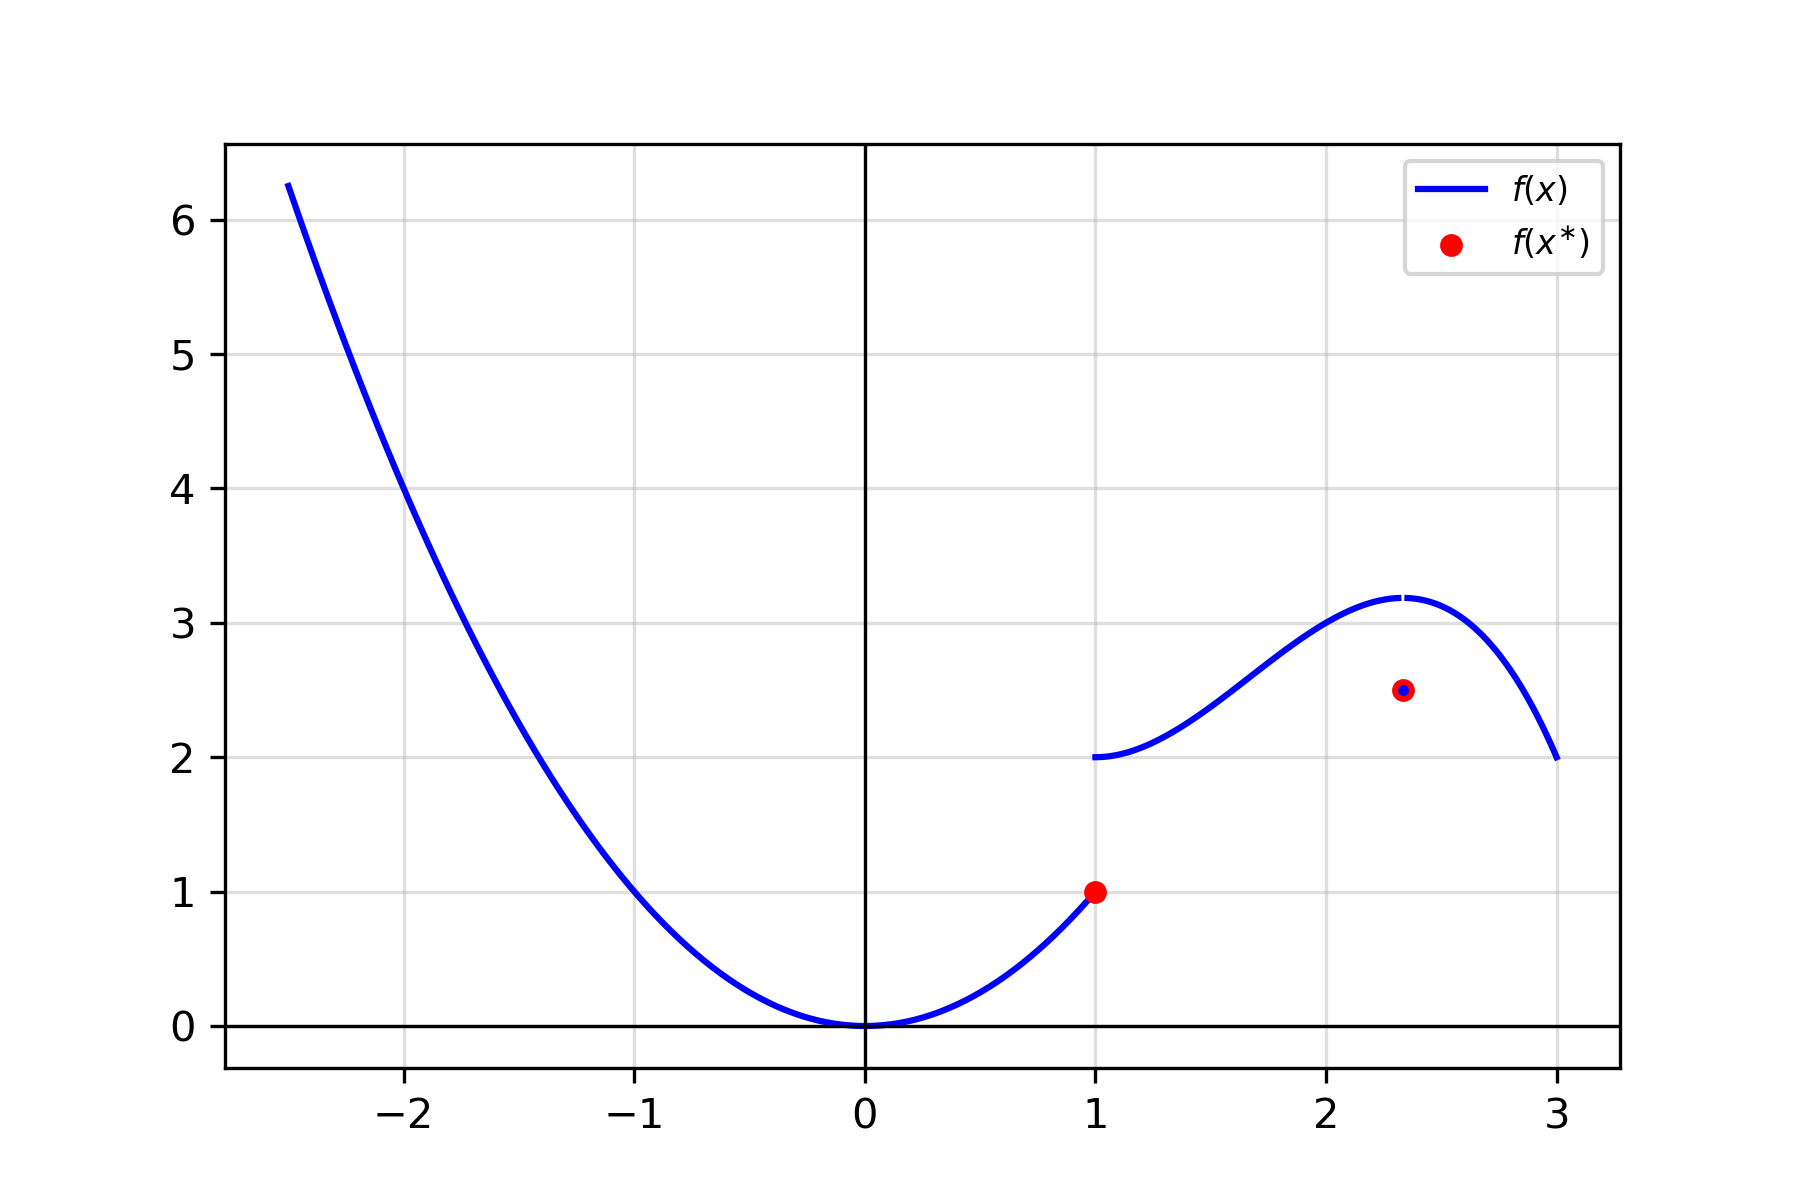
\includegraphics[width=0.5\textwidth]{figures/example_lsc.png}
\end{example}

\subsection{Koersivitet}
En koersiv funksjon er intuitivt en funksjon som "går mot uendelig" når vi beveger oss mot kanten av definisjonsmengden hvor \( f \) er definert.

\begin{definition}{Koersivitet}{coercive}
	En funksjon \(f: \Omega \to \R\) er koersiv hvis for alle \(y \in \R\) er nivåmengden \(\mathcal{L}_f(y) = \{x \in \Omega | f(x) \leq y\}\) kompakt.

	\[
		\lim_{\norm{x} \to +\infty} f(x) = +\infty
	\]
\end{definition}

\subsection{Konveksitet, kvasi-konveksitet og konvekse mengder}

Konveksitet er et viktig begrep i optimering og matematikk generelt. Det refererer til formen på en funksjon eller en mengde.
\begin{itemize}
	\item En konveks funksjon har en bue som vender oppover.
	\item En konkav funksjon har en bue som vender nedover.
	\item En konveks mengde er en mengde der enhver linje mellom to punkter i mengden også ligger helt innenfor mengden.
\end{itemize}

\begin{definition}{Konveks funksjon}{convex_function}
	En funksjon \(f: \R^n \to \R\) er:
	\begin{align*}
		f(\lambda x + (1-\lambda)y) & \leq \lambda f(x) + (1-\lambda)f(y) \quad \forall x, y \in \R^n, \lambda \in [0, 1] \tag{Konveks}                  \\
		f(\lambda x + (1-\lambda)y) & < \lambda f(x) + (1 - \lambda)f(y) \quad \forall x, y \in \R^n, \lambda \in (0, 1), x \neq y \tag{Strengt konveks}
	\end{align*}
\end{definition}

\begin{remark}{Konveksitet med indre-produkt notasjon}{convex_inner_product}
	En funksjon  \(f: \R^n \to \R\) er konveks hvis og bare hvis:
	\[
		f(y) - f(x) \geq  \langle \nabla f(x), y - x \rangle
	\]
	for alle  \(x, y \in \R^n\).
\end{remark}


\begin{remark}{Kvasi-konveks}{quasi_convex}
	En funksjon \(f: \R^d \to \R\) er kvasi-konveks hvis for alle \(x, y \in \R^n\) og \(\lambda \in (0, 1)\) har vi:

	\[
		f(\lambda x + (1 - \lambda)y) \leq \max\{f(x), f(y)\}
	\]

	En alternativ definisjon er at en funksjon er kvasi-konveks hvis alle nivåsettene er konvekse.

	\[
		\mathcal{L}_f(y) = \{x \in \R^n | f(x) \leq y\} \quad \text{er konveks for alle} \quad y \in \R
	\]

	\[
		\boxed{\underbrace{\forall \alpha \in \R, \mathcal{L}_f(\alpha) \text{ er konveks}}_{f \text{ er kvasi-konveks }}\Longleftrightarrow \forall x, y \in \R^d,\lambda \text{ s.a. } f(\lambda x + (1-\lambda)y) \leq \max \{ f(x), f(y) \}}
	\]
\end{remark}

\begin{definition}{Konveks sett}{convex_set}
	En mengde \(C \subset \R^n\) er (strengt) konveks når:

	\begin{align*}
		\lambda x + (1 - \lambda)y & \in C \quad \forall \; x, y \in C, \lambda \in [0, 1] \tag{Konveks}                   \\
		\lambda x + (1 - \lambda)y & \in C \quad \forall \; x, y \in C, \lambda \in (0, 1), x \neq y \tag{Strengt konveks}
	\end{align*}

\end{definition}

\begin{definition}{Konveks kombinasjon}{convex_combination}
	En konveks kombinasjon av punkter $x_1, x_2, \ldots, x_n$ i $\mathbb{R}^d$ er ethvert punkt på formen:
	\[
		\sum_{i=1}^n \lambda_i x_i \quad \text{der} \quad \lambda_i \geq 0, \sum_{i=1}^n \lambda_i = 1
	\]
\end{definition}

\begin{remark}{Karakterisering av deriverbare konvekse funksjoner}{convex-characterization}
	For en deriverbar funksjon  \(f: \R^n \to \R\) er følgende ekvivalente:
	\begin{itemize}
		\item  \(f\) er konveks
		\item For alle  \(x, y \in \R^n\) gjelder:
		      \[
			      f(y) \geq f(x) + \nabla f(x)^\top (y - x)
		      \]
	\end{itemize}
\end{remark}

\section{Ekvivalente utsagn for konvekse funksjoner}

La \(f:\mathbb{R}^n \to \mathbb{R}\) være en funksjon. Følgende utsagn er ekvivalente:
\begin{table}[H]
	\centering
	\small
	\begin{tabularx}{\textwidth}{|X|X|X|}
		\rowcolor{rem-color!25}
		\textbf{Ekvivalente Utsagn} & \textbf{Matematisk Definisjon} & \textbf{Forklaring og Intuisjon} \\
		\hline
		Geometrisk & 
		\( f(\lambda \symbf{x} + (1-\lambda)\symbf{y}) \le \lambda f(\symbf{x}) + (1-\lambda)f(\symbf{y}) \)  
		for alle \( \symbf{x},\symbf{y} \) i domenet og \( \lambda \in [0,1] \)
		& Grafen til \( f \) ligger under eller på sekantlinjene som forbinder to punkter på grafen. \\
		\hline
		Epi-graf &
		\(\operatorname{epi}(f) = \{ (\symbf{x},t)\in\mathbb{R}^n\times\mathbb{R} : f(\symbf{x})\le t \}\) er konveks.
		& Enhver konveks kombinasjon av punkter i epi-grafen tilhører også epi-grafen. \\
		\hline
		Første orden &
		\( f(\symbf{y}) \ge f(\symbf{x}) + \nabla f(\symbf{x})^\top (\symbf{y}-\symbf{x}) \)
		(gjelder dersom \( f \) er deriverbar)
		& Tangentplanet i ethvert punkt underestimerer \( f \) globalt, for alle \( \symbf{x},\symbf{y} \) i domenet. \\
		\hline
		Global optimalitet &
		Hvis \( f \) er konveks, er hvert lokalt minimum et globalt minimum.
		& En konsekvens av konveksitet: en konveks funksjon kan ikke ha ``isolerte'' lokale minima. (Merk at enkelte ikke-konvekse, quasi-konvekse funksjoner også kan ha denne egenskapen.) \\\hline
		Andre orden &
		\( \nabla^2 f(\symbf{x}) \succeq 0 \) for alle \( \symbf{x} \) i domenet 
		(dersom \( f \) er to ganger deriverbar)
		& Hessianmatrisen er positiv semidefinit, noe som via Taylorutvidelsen tilsier at funksjonen ikke ``bøyer'' seg nedover. \\
		\hline
		Subgradient &
		For alle \( \symbf{x} \) er \( \partial f(\symbf{x}) \neq \varnothing \) og for hvert \( s \in \partial f(\symbf{x}) \) gjelder 
		\( f(\symbf{y}) \ge f(\symbf{x}) + s^\top (\symbf{y}-\symbf{x}) \)
		& Selv om \( f \) ikke er deriverbar, gir tilstedeværelsen av subgradienter en lineær underestimering som karakteriserer konveksitet. 
		\\
		\hline
	\end{tabularx}
	\caption{Ekvivalente karakteriseringer av konvekse funksjoner, ordnet etter kompleksitet.}
	\label{tab:convex_equivalence}
\end{table}

\section{Geometriske objekter}
\subsection{Simplex}
Et simplex er en geometrisk figur som kan forstås som den enkleste formen i et gitt antall dimensjoner. For eksempel er et 0-simplex et punkt, et 1-simplex er en linje, et 2-simplex er en trekant, og så videre.

\begin{definition}{Simplex}{simplex}
	Et simplex i \( \mathbb{R}^n \) er et \( n \)-dimensjonalt objekt laget av \( n+1 \) punkter (hjørner) som ikke ligger i samme hyperplan.

	\begin{figure}[H]
		\centering
		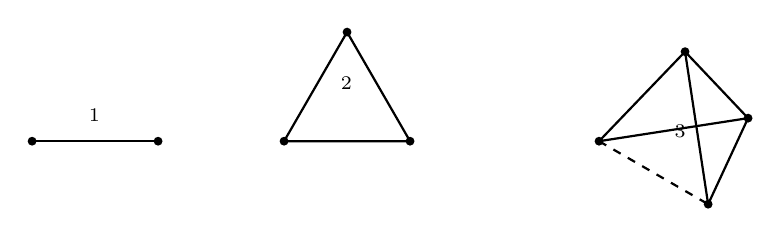
\begin{tikzpicture}[scale=0.8]
			% R1 simplex (line)
			\begin{scope}[shift={(-4,0)}]
				\draw[thick] (0,0) -- (2,0);
				\fill (0,0) circle (2pt);
				\fill (2,0) circle (2pt);
				\node[above] at (1,0) {$\R^1$};
			\end{scope}

			% R2 simplex (triangle)
			\begin{scope}[shift={(0,0)}]
				\draw[thick] (0,0) -- (2,0) -- (1,1.732) -- cycle;
				\fill (0,0) circle (2pt);
				\fill (2,0) circle (2pt);
				\fill (1,1.732) circle (2pt);
				\node[above] at (1,0.5) {$\R^2$};
			\end{scope}

			% R3 simplex (tetrahedron)
			\begin{scope}[shift={(5,0)}, x={(0.866cm,-0.5cm)}, y={(0.866cm,0.5cm)}, z={(0cm,1cm)}]
				% Back triangle
				\draw[thick,dashed] (0,0,0) -- (2,0,0);
				\draw[thick] (2,0,0) -- (1,1.732,0) -- (0,0,0);
				% Vertical edges to top point
				\draw[thick] (0,0,0) -- (1,0.577,1.633);
				\draw[thick] (2,0,0) -- (1,0.577,1.633);
				\draw[thick] (1,1.732,0) -- (1,0.577,1.633);
				% Points
				\fill (0,0,0) circle (2pt);
				\fill (2,0,0) circle (2pt);
				\fill (1,1.732,0) circle (2pt);
				\fill (1,0.577,1.633) circle (2pt);
				\node[above] at (1,0.5,0) {$\R^3$};
			\end{scope}
		\end{tikzpicture}
		\caption{Simplex i ulike dimensjoner.}
	\end{figure}
\end{definition}

\chapter{Konveksitet}

\section{Konvekse Mengder}

\subsection{Definisjon}
\begin{definition}{Konveks Mengde}{convex_set}
    En mengde $C \subset \mathbb{R}^n$ er \textbf{konveks} hvis, for ethvert par punkter $x, y \in C$, ligger hele linjesegmentet som forbinder dem i $C$. Formelt:
    \[
    x, y \in C \quad \Longrightarrow \quad \alpha x + (1-\alpha) y \in C \quad \text{for alle}~\alpha \in [0, 1].
    \]
    Ekvivalent kan man si at enhver konveks kombinasjon av punkter i $C$ forblir i $C$.
\end{definition}

\begin{figure}[htb]
    \centering
    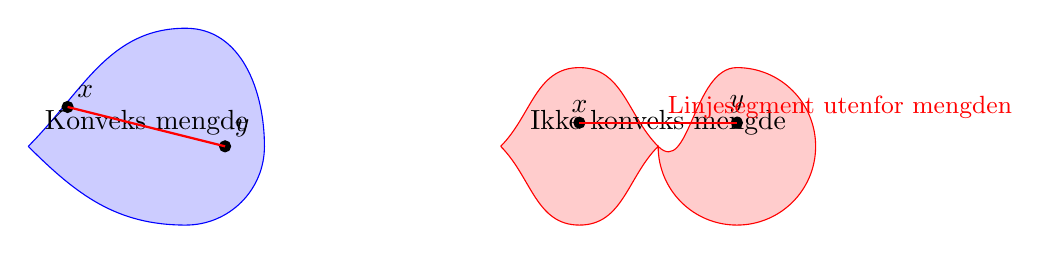
\begin{tikzpicture}
        % Convex set
        \draw[fill=blue!20, draw=blue] (0,0) to[out=45, in=180] (2,1.5) to[out=0, in=90] (3,0) to[out=270, in=0] (2,-1) to[out=180, in=315] (0,0);
        \node at (1.5, 0.3) {Konveks mengde};
        \filldraw[black] (0.5,0.5) circle (2pt) node[above right] {$x$};
        \filldraw[black] (2.5,0) circle (2pt) node[above right] {$y$};
        \draw[thick, red] (0.5,0.5) -- (2.5,0);
        
        % Non-convex set
        \begin{scope}[xshift=6cm]
            \draw[fill=red!20, draw=red] (0,0) to[out=45, in=180] (1,1) to[out=0, in=135] (2,0) to[out=315, in=180] (3,1) to[out=0, in=90] (4,0) to[out=270, in=0] (3,-1) to[out=180, in=270] (2,0) to[out=225, in=0] (1,-1) to[out=180, in=315] (0,0);
            \node at (2, 0.3) {Ikke-konveks mengde};
            \filldraw[black] (1,0.3) circle (2pt) node[above] {$x$};
            \filldraw[black] (3,0.3) circle (2pt) node[above] {$y$};
            \draw[thick, red] (1,0.3) -- (3,0.3);
            \node[red, right] at (2,0.5) {\small Linjesegment utenfor mengden};
        \end{scope}
    \end{tikzpicture}
    \caption{Illustrasjon av konvekse og ikke-konvekse mengder}
    \label{fig:convex_sets}
\end{figure}


\subsection{Eksempler}
\begin{example}{Vanlige Konvekse Mengder}{common_convex_sets}
    \begin{itemize}
        \item \textbf{Euklidske Kuler}: $\bigl\{ x : \|x - x_0\|\le r \bigr\}$ er konvekse fordi linjesegmenter mellom to punkter i en kule forblir inni.
        \item \textbf{Polyedre}: $\{x : A x \le b\}$ (ulikheter forstått komponentvis) er konvekse. Polytoper og simplekser er spesielle eksempler.
        \item \textbf{Affine Underrom}: $\{x : A x = b\}$ er konvekse.
        \item \textbf{Halvrom}: $\{x \in \mathbb{R}^n : a^T x \leq b\}$ er konvekse.
        \item \textbf{Kjegler}: $\{tx : t \geq 0, x \in C\}$ der $C$ er konveks er konvekse.
    \end{itemize}
\end{example}

\subsection{Operasjoner som Bevarer Konveksitet}
\begin{theorem}{Konveksitetsbevarende Operasjoner}{convexity_preserving}
    Følgende operasjoner bevarer konveksitet av mengder:
    \begin{itemize}
        \item \textbf{Snitt}: Snittet av enhver samling konvekse mengder er konveks.
        \item \textbf{Lineære eller Affine Avbildninger}: Hvis $T$ er en lineær (eller affin) transformasjon, og $C$ er konveks, er $T(C)$ konveks.
        \item \textbf{Minkowski Sum}: For konvekse $C_1,C_2$, er Minkowski-summen $\{x_1 + x_2 : x_1\in C_1, x_2\in C_2\}$ konveks.
        \item \textbf{Skalering og Translasjon}: For enhver $\alpha \in \mathbb{R}$ og $b \in \mathbb{R}^n$, er både $\alpha C$ og $C + b$ konvekse.
    \end{itemize}
\end{theorem}

\subsection{Ekstremalpunkter, Flater og Separasjon}
\begin{definition}{Ekstremalpunkt}{extreme_point}
    Et \textbf{ekstremalpunkt} i en konveks mengde $C$ er et punkt som ikke ligger i noe åpent linjesegment inneholdt i $C$ (bortsett fra det trivielle segmentet som starter og slutter i punktet selv).
\end{definition}

\begin{theorem}{Separasjonsteoremet}{separation_theorem}
    La $C$ og $D$ være disjunkte ikke-tomme konvekse mengder i $\mathbb{R}^n$.
    \begin{enumerate}
        \item Hvis $C$ er åpen, eksisterer det en ikke-null $p \in \mathbb{R}^n$ og $\alpha \in \mathbb{R}$ slik at $p^T x < \alpha \leq p^T y$ for alle $x \in C$ og $y \in D$.
        \item Hvis $C$ og $D$ er lukket og minst én er kompakt, eksisterer det en ikke-null $p \in \mathbb{R}^n$ og $\alpha, \beta \in \mathbb{R}$ slik at $p^T x \leq \alpha < \beta \leq p^T y$ for alle $x \in C$ og $y \in D$.
    \end{enumerate}
\end{theorem}

\begin{figure}[htb]
    \centering
    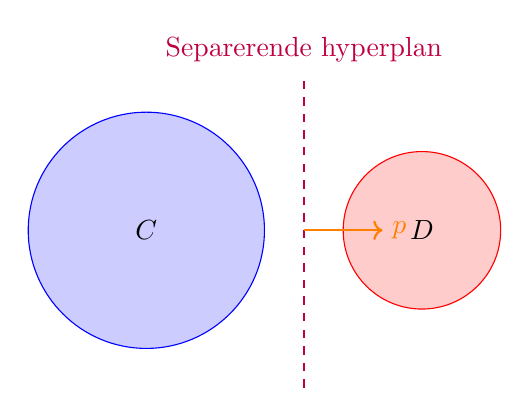
\begin{tikzpicture}
        % Første mengde (konveks)
        \draw[fill=blue!20, draw=blue] (0,0) circle (1.5);
        \node at (0, 0) {$C$};
        
        % Andre mengde (konveks)
        \draw[fill=red!20, draw=red] (3.5,0) circle (1);
        \node at (3.5, 0) {$D$};
        
        % Separerende hyperplan
        \draw[thick, dashed, purple] (2,-2) -- (2,2);
        \node[purple] at (2, 2.3) {Separerende hyperplan};
        
        % Normalvektor til hyperplanet
        \draw[->, thick, orange] (2,0) -- (3,0);
        \node[orange, right] at (3, 0) {$p$};
    \end{tikzpicture}
    \caption{Separasjon av to konvekse mengder med et hyperplan}
    \label{fig:separation}
\end{figure}

\section{Konvekse Funksjoner}

\subsection{Definisjon}
\begin{definition}{Konveks Funksjon}{convex_function}
    En funksjon $f: C \to \mathbb{R}$, med $C \subset \mathbb{R}^n$ konveks, er \textbf{konveks} hvis
    \[
    f\bigl(\alpha x + (1-\alpha) y \bigr) \;\le\; \alpha\, f(x) \;+\;(1-\alpha)\, f(y)\quad \text{for alle }x,y \in C,\;\alpha \in [0, 1].
    \]
    Intuitivt ligger grafen til $f$ "under korden" som forbinder to punkter på grafen.
\end{definition}

\begin{figure}[htb]
  \centering
  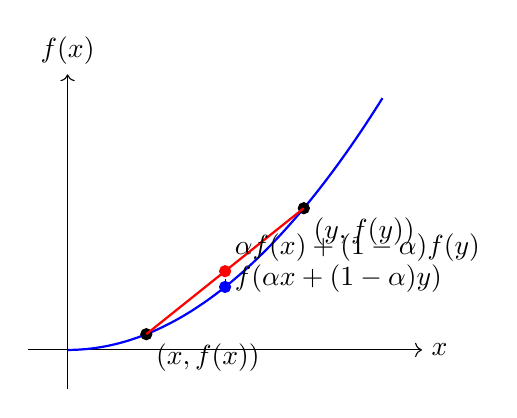
\begin{tikzpicture}
    % Axes
    \draw[->] (-0.5,0) -- (4.5,0) node[right] {$x$};
    \draw[->] (0,-0.5) -- (0,3.5) node[above] {$f(x)$};
    
    % Convex function (parabola)
    \draw[thick, blue] plot [domain=0:4, samples=100] (\x, {0.2*\x*\x});
    
    % Points on the function
    \filldraw[black] (1,0.2) circle (2pt) node[below right] {$(x,f(x))$};
    \filldraw[black] (3,1.8) circle (2pt) node[below right] {$(y,f(y))$};
    
    % Chord
    \draw[red, thick] (1,0.2) -- (3,1.8);
    
    % Midpoint on chord
    \filldraw[red] (2,1) circle (2pt);
    
    % Point on function at same x
    \filldraw[blue] (2,0.8) circle (2pt);
    
    % Vertical line connecting points
    \draw[dashed] (2,0.8) -- (2,1);
    
    % Labels
    \node[right] at (2,0.9) {$f(\alpha x + (1-\alpha)y)$};
    \node[above right] at (2,1) {$\alpha f(x) + (1-\alpha)f(y)$};
  \end{tikzpicture}
  \caption{En konveks funksjon ligger under korden som forbinder to punkter på dens graf}
  \label{fig:convex_function}
\end{figure}

\subsection{Ekvivalente Karakteriseringer}
\begin{theorem}{Karakteriseringer av Konveksitet}{convexity_characterizations}
  For en funksjon $f: C \to \mathbb{R}$ på et konvekst domene $C$:
  \begin{itemize}
    \item \textbf{Førsteordens Betingelse} (når $f$ er deriverbar):
    \[
    f(y)\;\ge\; f(x) + \nabla f(x)^\mathsf{T}\,(y - x), \quad \text{for alle }x, y \in C.
    \]
    Med ord: den lineære approksimasjonen (tangenten) ved $x$ er en global undereestimator av $f$.
    
    \item \textbf{Andreordens Betingelse} (når $f$ er to ganger deriverbar):
    \[
    \nabla^2 f(x)\; \text{er positiv semidefinitt for alle }x \in C.
    \]
    Det vil si at Hessian-matrisen er positiv semidefinitt overalt i $C$.
  \end{itemize}
\end{theorem}

\begin{figure}[htb]
  \centering
  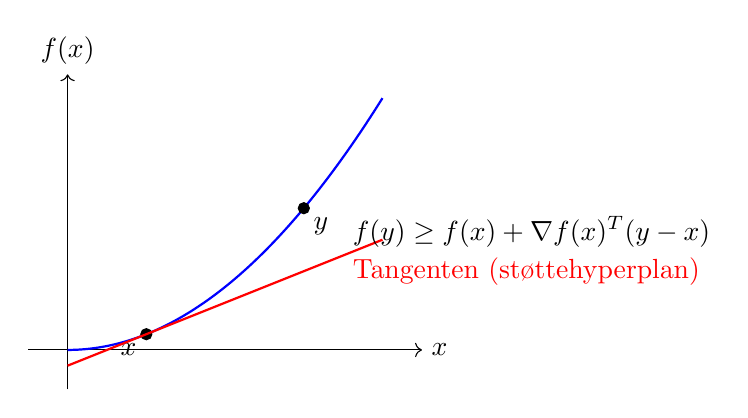
\begin{tikzpicture}
    % Axes
    \draw[->] (-0.5,0) -- (4.5,0) node[right] {$x$};
    \draw[->] (0,-0.5) -- (0,3.5) node[above] {$f(x)$};
    
    % Convex function (parabola)
    \draw[thick, blue] plot [domain=0:4, samples=100] (\x, {0.2*\x*\x});
    
    % Point on the function
    \filldraw[black] (1,0.2) circle (2pt) node[below left] {$x$};
    \filldraw[black] (3,1.8) circle (2pt) node[below right] {$y$};
    
    % Tangent at x
    \draw[red, thick] plot [domain=0:4, samples=100] (\x, {0.2*1*1 + 0.4*1*(\x-1)});
    
    % Labels
    \node[right] at (3.5,1.5) {$f(y) \geq f(x) + \nabla f(x)^T(y-x)$};
    \node[red, right] at (3.5,1) {Tangenten (støttehyperplan)};
  \end{tikzpicture}
  \caption{Førsteordens karakterisering av konveksitet: funksjonen ligger over sine tangentplan}
  \label{fig:first_order}
\end{figure}

\subsection{Eksempler}
\begin{example}{Vanlige Konvekse Funksjoner}{common_convex_functions}
  \begin{itemize}
    \item \textbf{Lineære eller Affine Funksjoner}: $f(x) = c^\mathsf{T} x + \beta$ er konvekse (og også konkave).
    \item \textbf{Normer}: $f(x) = \|x\|_p$ for $p \geq 1$ er konvekse.
    \item \textbf{Kvadratiske Former}: $f(x) = x^\mathsf{T} Q x$ er konveks hvis og bare hvis $Q$ er positiv semidefinitt.
    \item \textbf{Eksponential}: $f(x) = e^{\alpha x}$ (i én dimensjon) eller $f(x)= \exp(\langle \alpha, x \rangle)$ (multidimensjonal) er konveks.
    \item \textbf{Logaritmisk Barriere}: $f(x) = -\log(x)$ på $\mathbb{R}_{++}$ er konveks.
    \item \textbf{Entropi}: $f(x) = x\log(x)$ på $\mathbb{R}_{++}$ er konveks.
  \end{itemize}
\end{example}

\begin{table}[htb]
  \centering
  \begin{tabular}{|l|l|c|}
    \hline
    \textbf{Funksjon} & \textbf{Domene} & \textbf{Konveksitet} \\
    \hline
    $f(x) = c^Tx + b$ & $\mathbb{R}^n$ & Konveks og konkav \\
    $f(x) = \|x\|_p$, $p \geq 1$ & $\mathbb{R}^n$ & Konveks \\
    $f(x) = x^TQx$, $Q \succeq 0$ & $\mathbb{R}^n$ & Konveks \\
    $f(x) = e^x$ & $\mathbb{R}$ & Konveks \\
    $f(x) = -\log(x)$ & $\mathbb{R}_{++}$ & Konveks \\
    $f(x) = x\log(x)$ & $\mathbb{R}_{++}$ & Konveks \\
    $f(x) = 1/x$ & $\mathbb{R}_{++}$ & Konveks \\
    $f(x) = \max\{x_1, x_2, \ldots, x_n\}$ & $\mathbb{R}^n$ & Konveks \\
    \hline
  \end{tabular}
  \caption{Eksempler på vanlige konvekse funksjoner}
  \label{tab:convex_functions}
\end{table}

\subsection{Vanlige Egenskaper}
\begin{theorem}{Operasjoner som Bevarer Funksjonskonveksitet}{function_convexity_preserving}
  Følgende operasjoner bevarer funksjonskonveksitet:
  \begin{itemize}
    \item \textbf{Ikke-negative Vektede Summer}: Hvis $f_1, f_2, \ldots, f_n$ er konvekse og $\alpha_1, \alpha_2, \ldots, \alpha_n \geq 0$, da er $\sum_{i=1}^n \alpha_i f_i$ konveks.
    
    \item \textbf{Punktvis Maksimum}: Hvis $f_1, f_2, \ldots, f_n$ er konvekse, da er $\max\{f_1, f_2, \ldots, f_n\}$ konveks.
    
    \item \textbf{Punktvis Supremum}: Hvis $f_\alpha$ er konveks for hver $\alpha \in A$, da er $\sup_{\alpha \in A} f_\alpha$ konveks.
    
    \item \textbf{Sammensetning med Affin Funksjon}: Hvis $f$ er konveks og $A$ er en matrise og $b$ er en vektor, da er $g(x) = f(Ax + b)$ konveks.
    
    \item \textbf{Minimering over Noen Variabler}: Hvis $f(x,y)$ er felles konveks i $(x,y)$, da er $g(x) = \inf_y f(x,y)$ konveks i $x$.
  \end{itemize}
\end{theorem}

\subsection{Subgradienter (Generelle Derivater)}
\begin{definition}{Subgradient}{subgradient}
  For en konveks funksjon $f: C \to \mathbb{R}$, er en vektor $g \in \mathbb{R}^n$ en \textbf{subgradient} av $f$ ved $x \in C$ hvis
  \[
  f(y)\;\ge\; f(x)\;+\; g^\mathsf{T}\,(y-x),\quad \forall y \in C.
  \]
  Mengden av alle subgradienter av $f$ ved $x$ kalles \textbf{subdifferensialet} av $f$ ved $x$, og betegnes med $\partial f(x)$.
\end{definition}

\begin{figure}[htb]
  \centering
  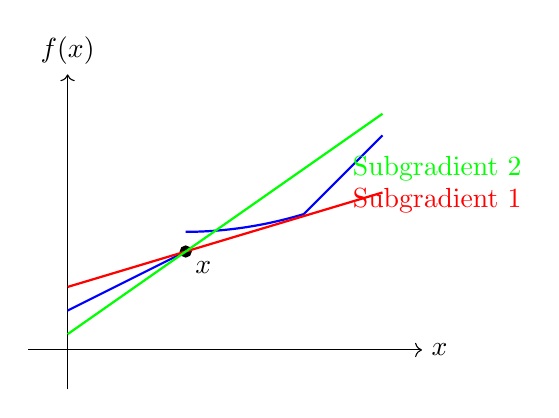
\begin{tikzpicture}
    % Axes
    \draw[->] (-0.5,0) -- (4.5,0) node[right] {$x$};
    \draw[->] (0,-0.5) -- (0,3.5) node[above] {$f(x)$};
    
    % Convex function (piecewise)
    \draw[thick, blue] plot [domain=0:1.5, samples=50] (\x, {0.5*\x + 0.5});
    \draw[thick, blue] plot [domain=1.5:3, samples=50] (\x, {1.5 + 0.1*(\x-1.5)^2});
    \draw[thick, blue] plot [domain=3:4, samples=50] (\x, {1.5 + 0.1*(3-1.5)^2 + 1*(\x-3)});
    
    % Point of non-differentiability
    \filldraw[black] (1.5,1.25) circle (2pt) node[below right] {$x$};
    
    % Subgradients
    \draw[red, thick] plot [domain=0:4, samples=50] (\x, {1.25 + 0.3*(\x-1.5)});
    \draw[green, thick] plot [domain=0:4, samples=50] (\x, {1.25 + 0.7*(\x-1.5)});
    
    % Labels
    \node[red, right] at (3.5,1.9) {Subgradient 1};
    \node[green, right] at (3.5,2.3) {Subgradient 2};
  \end{tikzpicture}
  \caption{Subgradienter av en konveks funksjon ved et punkt der den ikke er deriverbar}
  \label{fig:subgradients}
\end{figure}

\section{Grunnleggende Resultater og Implikasjoner}

\subsection{Jensens Ulikhet}
\begin{theorem}{Jensens Ulikhet}{jensens_inequality}
  For enhver konveks funksjon $f: C \to \mathbb{R}$ og punkter $x_1, x_2, \ldots, x_k \in C$:
  \[
  f\Bigl(\sum_{i=1}^k \alpha_i x_i \Bigr) \;\le\; \sum_{i=1}^k \alpha_i\, f(x_i),
  \]
  når $\alpha_i\ge 0$ og $\sum_{i=1}^k \alpha_i=1$.
  
  For stokastiske variabler, hvis $X$ er en stokastisk variabel med verdier i $C$ og $f$ er konveks, da:
  \[
  f(\mathbb{E}[X]) \leq \mathbb{E}[f(X)]
  \]
  forutsatt at forventningsverdiene eksisterer.
\end{theorem}

\subsection{Konveks Programmering}
\begin{definition}{Konvekst Optimeringsproblem}{convex_optimization_problem}
  Et konvekst optimeringsproblem har formen:
  \begin{mini*}
    {x \in \mathbb{R}^n}{f(x)}{}{}
    \addConstraint{g_i(x) \leq 0,}{i = 1, \ldots, m}
    \addConstraint{h_j(x) = 0,}{j = 1, \ldots, p}
  \end{mini*}
    
  hvor $f$ og $g_i$ er konvekse funksjoner, og $h_j(x) = a_j^Tx - b_j$ er affine funksjoner.
\end{definition}

\begin{theorem}{Egenskaper ved Konveks Optimering}{convex_optimization_properties}
  For et konvekst optimeringsproblem:
  \begin{enumerate}
    \item Enhver lokal minimerer er en global minimerer.
    \item Mengden av minimerere, hvis ikke-tom, er konveks.
    \item Hvis $f$ er strengt konveks, har problemet høyst én løsning.
    \item KKT-betingelsene er nødvendige og tilstrekkelige for optimalitet (under kvalifikasjonsbetingelser).
  \end{enumerate}
\end{theorem}

\subsection{Epigraf-Formulering}
\begin{definition}{Epigraf}{epigraph}
  \textbf{Epigrafen} til en funksjon $f: C \to \mathbb{R}$ er mengden
  \[
  \mathrm{epi}(f) \;=\; \{(x,t)\mid x\in C,\; t\ge f(x)\}.
  \]
  En funksjon $f$ er konveks hvis og bare hvis $\mathrm{epi}(f)$ er en konveks mengde i $\mathbb{R}^{n+1}$.
\end{definition}

\begin{figure}[htb]
  \centering
  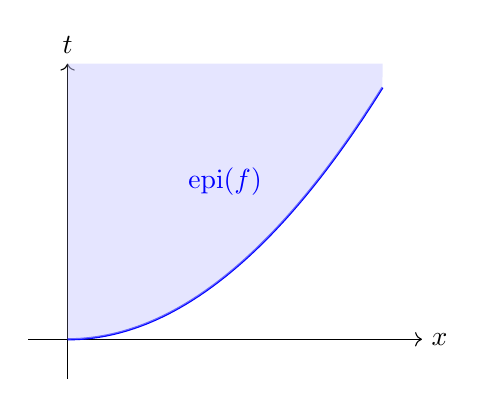
\begin{tikzpicture}
    % Axes
    \draw[->] (-0.5,0) -- (4.5,0) node[right] {$x$};
    \draw[->] (0,-0.5) -- (0,3.5) node[above] {$t$};
    
    % Convex function
    \draw[thick, blue] plot [domain=0:4, samples=100] (\x, {0.2*\x*\x});
    
    % Epigraph
    \fill[blue!20, opacity=0.5] (0,0) -- plot [domain=0:4, samples=100] (\x, {0.2*\x*\x}) -- (4,3.5) -- (0,3.5) -- cycle;
    
    % Label
    \node[blue] at (2,2) {epi$(f)$};
  \end{tikzpicture}
  \caption{Epigrafen til en konveks funksjon}
  \label{fig:epigraph}
\end{figure}

\subsection{Dualitet i Konveks Optimering}
\begin{definition}{Lagrangian-Dualitet}{lagrangian_duality}
  For det konvekse optimeringsproblem
    \begin{mini}
      {x}{f(x)}{}{}
      \addConstraint{g_i(x)}{\leq 0,}{i = 1,\ldots,m}
      \addConstraint{Ax}{= b}{}
    \end{mini}
  er Lagrangian-funksjonen $\mathcal{L}(x,\lambda,\nu) = f(x) + \sum_{i=1}^m \lambda_i g_i(x) + \nu^T(Ax-b)$ hvor $\lambda_i \geq 0$. 
  Dualfunksjonen er $g(\lambda,\nu) = \inf_x L(x,\lambda,\nu)$ og dualproblemet er
    \begin{maxi}
      {\lambda,\nu}{g(\lambda,\nu)}{}{}
      \addConstraint{\lambda}{\geq 0}{}
    \end{maxi}
\end{definition}

\begin{theorem}{Sterk Dualitet}{strong_duality}
  Hvis et konvekst optimeringsproblem tilfredsstiller Slaters betingelse (dvs. det eksisterer et strengt mulig punkt), da gjelder sterk dualitet: de optimale verdiene av primal- og dualproblemet er like.
\end{theorem}

\section{Konveksitet - Sammendrag}
% First table: Basic Concepts
\begin{table}[H]
  \centering
  \begin{tabular}{|p{3cm}|p{5cm}|p{6cm}|}
    \hline
    \rowcolor{blue!25}
    \textbf{Konsept} & \textbf{Definisjon} & \textbf{Matematisk Formulering} \\
    \hline
    Konveks Mengde & En mengde hvor ethvert linjesegment mellom to punkter i mengden ligger helt i mengden &
    \(C\subset \mathbb{R}^n\) er konveks hvis:
    \[\forall x,y\in C,\;\alpha\in [0,1]:\] 
    \[\alpha x + (1-\alpha) y\in C\] \\
    \hline
    \rowcolor{blue!5}
    Konveks Funksjon & En funksjon hvor grafen ligger under linjesegmentet mellom to punkter på grafen &
    \(f: C \to \mathbb{R}\) er konveks hvis:
    \[f(\alpha x + (1-\alpha) y)\;\le\]\[\alpha f(x) + (1-\alpha) f(y)\] 
    for alle \(x,y\in C,\;\alpha\in [0,1]\) \\
    \hline
  \end{tabular}
  \caption{Grunnleggende konsepter innen konveksitet}
  \label{tab:basic_concepts}
\end{table}

% Second table: Characterizations
\begin{table}[H]
  \centering
  \begin{tabular}{|p{3cm}|p{5cm}|p{6cm}|}
    \hline
    \rowcolor{rem-color!25}
    \multicolumn{3}{|l|}{\textbf{Karakteriseringer av Konveksitet}} \\
    \hline
    \rowcolor{rem-color!5}
    1. Ord. Bet. & Tangentapproks. ved ethvert punkt er en global underestimator &
    For deriverbar \(f\), konveksitet er ekvivalent med:
    \[f(y)\;\ge\; f(x) + \nabla f(x)^\mathsf{T} (y - x)\]
    \[\forall x,y \in C\] \\
    \hline
    2. Ord. Bet. & \(H_f(x)\) er pos. semidefinit overalt i \(C\) &
    For \(f \in C^2\), konveksitet er ekvivalent med:
    \[\nabla^2 f(x) \succeq 0\quad \forall x \in C\] \\
    \hline
  \end{tabular}
  \caption{Karakteriseringer av konveksitet}
  \label{tab:characterizations}
\end{table}

% Third table: Important Results
\begin{table}[H]
  \centering
  \begin{tabular}{|p{3cm}|p{5cm}|p{6cm}|}
    \hline
    \rowcolor{cor-color!25}
    \multicolumn{3}{|l|}{\textbf{Viktige Resultater}} \\
    \hline
    \rowcolor{cor-color!5}
    Jensens Ulikhet & Funksjonsverdien av et vektet gjennomsnitt er mindre enn \newline
    eller lik det vektede gjennomsnittet av funksjonsverdiene &
    For konveks \(f\) og vekter \(\alpha_i \geq 0\) med \(\sum_i \alpha_i = 1\):
    \[f\Bigl(\sum_i \alpha_i x_i\Bigr)\;\le\;\sum_i \alpha_i f(x_i)\] \\
    \hline
    Epigraf & Mengden av alle punkter som ligger på eller over grafen til funksjonen &
    \(\mathrm{epi}(f)=\{(x,t) \mid x\in\mathrm{dom}(f), t\ge f(x)\}\)
    
    \(f\) er konveks \(\Leftrightarrow\) \(\mathrm{epi}(f)\) er konveks \\
    \hline
    \rowcolor{cor-color!5}
    Subgradient & Generalisering av gradient for ikke-deriverbare funksjoner &
    En vektor \(g\) er en subgradient av konveks \(f\) ved \(x\) hvis:
    \[f(y)\;\ge\; f(x) + g^\mathsf{T}(y-x)\quad \forall y \in C\] \\
    \hline
  \end{tabular}
  \caption{Viktige resultater innen konveksitet}
  \label{tab:important_results}
\end{table}

% Fourth table: Optimization Theory
\begin{table}[H]
  \centering
  \begin{tabular}{|p{3cm}|p{5cm}|p{6cm}|}
    \hline
    \rowcolor{prop-color!25}
    \multicolumn{3}{|l|}{\textbf{Optimeringsteori}} \\
    \hline
    \rowcolor{prop-color!5}
    Lokale/Globale\newline Minima & For konvekse problemer er\newline ethvert lokalt minimum\newline også et globalt minimum & 
    For konveks \(f\) på konveks \(C\):\newline\quad\(\text{lokal min} \iff \text{global min}\) \\
    \hline
    Sterk Dualitet & Under visse betingelser er det ingen dualitetsgap &
    Under Slaters betingelse: 
    \[\text{primal opt.} = \text{dual opt.}\] \\
    \hline
  \end{tabular}
  \caption{Optimeringsteori og konveksitet}
  \label{tab:optimization_theory}
\end{table}


\section{Betydning i Optimering}
Konveksitet er avgjørende i optimering av flere viktige grunner:

\begin{itemize}
    \item \textbf{Global Optimalitet}: Konvekse optimeringsproblemer har et unikt globalt minimum hvis streng konveksitet holder, siden ethvert lokalt minimum er globalt.
    
    \item \textbf{Forenklede Optimalitetsbetingelser}: Førsteordens optimalitetsbetingelser er tilstrekkelige for global optimalitet, noe som forenkler analyse og løsningsmetoder.
    
    \item \textbf{Algoritmisk Effektivitet}: Det finnes effektive algoritmer for å løse konvekse optimeringsproblemer, inkludert gradientmetoder, indrepunktsmetoder og proksimalmetoder.
    
    \item \textbf{Praktiske Anvendelser}: Mange praktiske problemer innen maskinlæring, kontrollteori, signalbehandling og finans kan formuleres som konvekse optimeringsproblemer eller tilnærmes av dem.
    
    \item \textbf{Dualitetsteori}: Konveksitet muliggjør kraftige dualitetsresultater som gir alternative løsningsmetoder og sensitivitetsanalyse.
\end{itemize}


\paragraph{Oppsummering av Konveksitet}
Konvekse mengder og funksjoner spiller en sentral rolle i optimering fordi de gir problemer som er relativt enkle å analysere og (ofte) mye enklere å løse, både teoretisk og algoritmisk. 
Den viktige egenskapen om at \emph{lokale minima er globale} gjør det mulig å forenkle beregningene betydelig og gir sterke konvergensegenskaper for standardalgoritmer som gradientmetoder, indrepunktsmetoder, subgradientmetoder, og så videre.

\chapter{Hva er optimering?}
\label{chap:what_is_optimization}

Optimering er et felt innen matematikken som handler om å finne den beste løsningen på et gitt problem, enten med eller uten restriksjoner på løsningsrommet.

Målet i et \emph{optimeringsproblem} er å finne en variabel \(x^\star \in \Omega\) som minimerer eller maksimerer en gitt funksjon \(f: \Omega \to \R\),
kalt \emph{mål\-funksjonen} eller \emph{kostnads\-funksjonen}.

\section{Optimeringsproblemer i \texorpdfstring{\(\R^d\)}{Rd}}

Mengden \(\Omega \subseteq \R^d\) betegner de tillatte løsningene og kalles ofte \emph{søkeområdet} eller den \emph{tillatte mengden (eng. feasible set)}.

\begin{definition}{Optimeringsproblemet \((P)\)}{def:optimization_problem}

	La \(f: \Omega \to \R\) være en funksjon vi ønsker å minimere eller maksimere, der \(\Omega \subseteq \R^d\) er mengden av tillatte (mulige) løsninger.
	\[
		\min_{x \in \Omega} f(x) \quad \text{eller} \quad \max_{x \in \Omega} f(x) \tag{P}
	\]

\end{definition}

Vi fokuserer hovedsakelig på minimeringsproblemer, siden maksimeringsproblemer enkelt kan omformuleres ved å erstatte \(f(x)\) med \(-f(x)\).
De fleste algoritmene vi diskuterer, er designet for å løse minimeringsproblemer.

\section{Ubundet og Bundet optimering}
Ulike problemtyper oppstår ut fra hvordan denne mengden \(\Omega\) er definert, og hvilke egenskaper funksjonen \(f\) har.

Vi skiller mellom tre hovedtyper av optimeringsproblemer:
\paragraph{Ubundet optimering} er den enkleste typen optimeringsproblemer, hvor man ikke har restriksjoner på variabelen \(\symbf{x}^\star\), hvor vi ønsker å minimere \(f(x)\) over hele rommet \(\R^d\).
\paragraph{Bundet optimering} er når vi har restriksjoner på den tillatte mengden \(\Omega \subseteq \R^d\). I motsetning til ubundet optimering kan vi ikke lenger søke over hele rommet \(\R^d\), men må holde oss innenfor spesifikke begrensninger.
Disse er ofte definert ved hjelp av ulikheter og likheter.
\begin{align*}
    g_i(x) &\leq 0, \quad i \in \mathcal{I} \quad \text{(ulikhetsrestriksjoner)} \\
    h_j(x) &= 0, \quad j \in \mathcal{E} \quad \text{(likhetsrestriksjoner)}
\end{align*}

Da kan vi definere den tillatte mengden \(\Omega\) som:
\[
    \Omega = \{ x \in \R^d \mid g_i(x) \leq 0, \, i \in \mathcal{I}, \quad h_j(x) = 0, \, j \in \mathcal{E} \}
\]

Under dette igjen kan vi igjen klassifisere 3 bundne optimeringsproblemtyper:
\subparagraph{Lineær programmering (LP)} Når \(f\) og restriksjonene er lineære.
\subparagraph{Ikke-lineær programmering (NLP)} Når én eller flere av \(f\), \(g_i\), eller \(h_j\) er ikke-lineære.
\subparagraph{Kvadratisk programmering (QP)} Når \(f\) er kvadratisk og restriksjonene er lineære.

\paragraph{Konveks optimering} En spesialklasse der \(f\) og \(\Omega\) er konvekse.
Dette forteller oss at enhver lokal løsning er global, løsningen er entydig hvis \(f\) er strengt konveks, og effektive algoritmer finnes.

\section{Globale og lokale løsninger}
\label{sec:global_and_local_solutions}
I optimeringsproblemer er det viktig å skille mellom globale og lokale løsninger. En global løsning er den beste løsningen i hele søkeområdet, mens en lokal løsning er den beste løsningen i et begrenset område rundt et punkt.


\subsection{Globale løsninger}
En global løsning er den beste løsningen i hele søkeområdet \(\Omega\). Dette betyr at det ikke finnes noen annen løsning i hele \(\Omega\) som gir en bedre verdi for funksjonen \(f\).

\begin{definition}{Globale løsninger}{global_solution}

	\medskip
	For en funksjon \(f: \Omega \to \R\) sier vi at \(\symbf{x}^\star \in \Omega\) er en global løsning av minimeringsproblemet~\eqref{eq:global_minimization_problem} hvis:

	\begin{align*}
		f(\symbf{x}^\star) & \leq f(\symbf{x}) \quad \forall \symbf{x} \in \Omega \tag{Global}                                      \\
		f(\symbf{x}^\star) & < f(\symbf{x}) \quad \forall \symbf{x} \in \Omega, \symbf{x} \neq \symbf{x}^\star \tag{Strengt Global}
	\end{align*}
\end{definition}

\subsubsection{Eksistens av globale løsninger}

En funksjon \(f: \Omega \subset \R^d \to \overline{\R}\) har en global løsning (minimum) i \(\Omega\) hvis den er:

\begin{itemize}
	\item \textbf{Nedre semi-kontinuerlig}: For alle \(x \in \Omega\) og alle sekvenser \((x_n)\) som konvergerer mot \(x\):
	      \[
		      f(x) \leq \liminf_{n \to \infty} f(x_n).
	      \]
	\item \textbf{Koersiv}: Det finnes en konstant \(M > 0\) slik at
	      \[
		      f(x) \geq M \quad \forall x \in \Omega.
	      \]
	      Dette sikrer at \(f\) ikke går mot \(-\infty\) når \(x\) går mot uendelig.
\end{itemize}

\begin{theorem}{Eksistens av globale løsninger}{existence_of_global_solution}
	La \(f: \Omega \subset \R^d \to \overline{\R}\) være nedre semi-kontinuerlig og koersiv på \(\Omega\). Da har \(f\) en global løsning (minimum) i \(\Omega\).
\end{theorem}

\subsection{Lokale løsninger}
En lokal løsning er den beste løsningen i et begrenset område rundt et punkt \(\symbf{x}^\star\).
For å avgjøre om \(\symbf{x}^\star\) er en lokal løsning, må vi undersøke om det finnes bedre løsninger i nærheten.
De fleste metoder for dette baseres på Taylor-utvikling \ref{thm:taylors_theorem}.


\begin{definition}{Lokal løsning}{}
	La \(f: \Omega \to \R\) være en funksjon.

	Vi sier at \(x^\star \in \Omega\) er en lokal løsning av optimeringsproblemet hvis, for en viss \(\varepsilon > 0\):

	\begin{align*}
		f(\symbf{x}^\star) & \leq f(\symbf{x}) \quad \forall \; \symbf{x} \in B(\symbf{x}^\star, \varepsilon) \cap \Omega,                                                  \\
		f(\symbf{x}^\star) & < f(\symbf{x}) \quad \forall \; \symbf{x} \in B(\symbf{x}^\star, \varepsilon) \cap \Omega, \symbf{x} \neq \symbf{x}^\star. \tag{Strengt lokal}
	\end{align*}

	hvor \(B(\symbf{x}^\star, \varepsilon)\) er en åpen kule med sentrum \(\symbf{x}^\star\) og radius \(\varepsilon\)~\ref{def:open_ball}.
\end{definition}

\subsubsection{Taylors teorem}
Taylor-utvikling er en metode for å tilnærme en funksjon ved hjelp av dens deriverte.
Den gir oss en måte å uttrykke funksjonen som en sum av dens verdier og deriverte i et punkt, noe som kan være nyttig for å analysere oppførselen til funksjonen i nærheten av det punktet.

Ved hjelp av Taylor-utvikling kan vi avgjøre om \(\symbf{x}^\star\) er en lokal løsning ved å sjekke om gradienten \(\nabla f(\symbf{x}^\star) = 0\) og Hesse-matrisen \(\nabla^2 f(\symbf{x}^\star)\)

\begin{theorem}{Taylors teorem}{taylors_theorem}
	Anta at \(f: \R^n \to \R\) med \(\mathbf{p}\in\R^n\), og la \(t\in[0,1]\).

	\medskip

	Hvis \(f\in\Ccal^1\) (én gang kontinuerlig deriverbar):
	\[
		f(\mathbf{x} + \mathbf{p}) = f(\mathbf{x}) + \nabla f(\mathbf{x}+t\mathbf{p})^\top \mathbf{p},
	\]

	Hvis \(f \in \Ccal^2\) (to ganger kontinuerlig deriverbar):

	\begin{align*}
		\nabla f(\mathbf{x} + \mathbf{p}) = \nabla f(\mathbf{x}) + \int_0^1 \nabla^2 f(\mathbf{x}+t\mathbf{p})\mathbf{p} dt, \\
		\boxed{f(\mathbf{x} + \mathbf{p}) = f(\mathbf{x}) + \nabla f(\mathbf{x})^\top \mathbf{p} + \frac{1}{2}\mathbf{p}^\top \nabla^2 f(\mathbf{x}+t\mathbf{p})\mathbf{p}}
	\end{align*}
\end{theorem}

\subsubsection{Isolerte lokale løsninger}
En isolert lokal løsning er en lokal løsning der det ikke finnes andre løsninger i nærheten. Dette betyr at det er en viss avstand fra \(\symbf{x}^\star\) til alle andre løsninger.

\begin{lemma}{Isolert lokal løsning}{isolated_local_solution}
	La \(f: \Omega \to \R\) være en funksjon.

	Hvis \(\symbf{x}^\star \in \Omega\) er en isolert lokal løsning, finnes det en \(\varepsilon > 0\) slik at:

	\[
		f(\symbf{x}^\star) \leq f(\symbf{x}) \quad \forall \; \symbf{x} \in B(\symbf{x}^\star, \varepsilon) \cap \Omega, \symbf{x} \neq \symbf{x}^\star.
	\]
\end{lemma}


\section{Veldefinerthet}
\begin{definition}{Veldefinert funksjon}{well_defined}
    La $f: X \to Y$ være en funksjon. Vi sier at $f$ er veldefinert hvis:
    \begin{enumerate}
        \item For hvert $x \in X$ eksisterer det nøyaktig én verdi $f(x) \in Y$.
        \item Funksjonen er entydig bestemt, det vil si at hvis $x_1 = x_2$ så er $f(x_1) = f(x_2)$.
    \end{enumerate}
    
    En operator eller en transformasjon er veldefinert hvis den tilfredsstiller de samme kravene: hver innverdi gir nøyaktig én utverdi, og like innverdier gir like utverdier.
\end{definition}

\chapter{Optimalitetsbetingelser}
\label{chap:optimality_conditions}
\section{Første Ordens Nødvendige Betingelser}

For en lokal løsning \(\mathbf{x}^\star\) må gradienten være null:

\begin{theorem}{First-Order Necessary Conditions}{first_order_necessary_conditions}
	Hvis \(\mathbf{x}^\star\) er et lokalt minimum, og \(f\) er kontinuerlig deriverbar rundt \(\mathbf{x}^\star\), da er:
	\[
		\nabla f(\mathbf{x}^\star) = 0.
	\]
\end{theorem}

\section{Andre Ordens Nødvendige Betingelser}

For en lokal løsning må både gradienten være null og Hesse-matrisen positiv definit:

\begin{theorem}{Second-Order Necessary Conditions}{second_order_necessary_conditions}
	Hvis \(\mathbf{x}^\star\) er et lokalt minimum, og \(f\) er to ganger kontinuerlig deriverbar rundt \(\mathbf{x}^\star\), da er:
	\[
		\nabla f(\mathbf{x}^\star) = 0 \quad \text{og} \quad \nabla^2 f(\mathbf{x}^\star) \succeq 0.
	\]
\end{theorem}

\section{Andre Ordens Tilstrekkelige Betingelser}

\begin{theorem}{Second-Order Sufficient Conditions}{second_order_sufficient_conditions}
	Hvis \(\nabla f(\mathbf{x}^\star) = 0\) og \(\nabla^2 f(\mathbf{x}^\star) \succ 0\) (positiv definit), da er \(\mathbf{x}^\star\) et \emph{strengt lokalt minimum}.

	\medskip

	Det vil si at det finnes en \(\varepsilon > 0\) slik at:
	\[
		f(\mathbf{x}^\star) < f(\mathbf{x})  \quad \forall \; \mathbf{x} \in B(\mathbf{x}^\star, \varepsilon) \cap \Omega, \mathbf{x} \neq \mathbf{x}^\star.
	\]
\end{theorem}

\section{Stasjonære punkter}
Stasjonære punkter er punkter der gradienten til funksjonen er null. Dette betyr at det ikke er noen retning der funksjonen øker eller minker, og det kan være et minimum, maksimum eller et sadelpunkt.

\begin{definition}{Stasjonære punkter}{stationary_points}
	La \(f: \Omega \to \R\) være en funksjon. Et punkt \(\symbf{x}^\star \in \Omega\) er et stasjonært punkt hvis:
	\[
		\nabla f(\symbf{x}^\star) = 0.
	\]
	Dette betyr at gradienten til \(f\) i punktet \(\symbf{x}^\star\) er lik null.
\end{definition}

\subsection{Konvergens til stasjonære punkter}
Når vi bruker iterative metoder for å finne minimum av en funksjon \(f\), ønsker vi å vite om algoritmen vil konvergere til det stasjonære punktet \(\symbf{x}^\star\).

\begin{theorem}{Konvergens til stasjonære punkter}{convergence_to_stationary_points}
	Anta at \(f: \R^d \to \R\) er en kontinuerlig deriverbar funksjon, og at følgende betingelser er oppfylt:
	\begin{enumerate}
		\item \(\Omega\) er en lukket og begrenset mengde.
		\item \(f(\symbf{x})\) er koersiv.
		\item \(f(\symbf{x})\) er nedre semi-kontinuerlig.
		\item \(\nabla f(\symbf{x})\) eksisterer og er Lipschitz-kontinuerlig.
		\item \(\nabla^2 f(\symbf{x})\) eksisterer og er Lipschitz-kontinuerlig.
	\end{enumerate}
	Da konvergerer sekvensen \((\symbf{x}_k)\) generert av en optimaliseringsalgoritme til et stasjonært punkt \(\symbf{x}^\star\) i \(\Omega\).
	\[
		\lim_{k \to \infty} \|\nabla f(\symbf{x}_k)\| = 0.
	\]

	hvor \(\symbf{x}_k\) er iteratene generert av en optimaliseringsalgoritme, og \(\symbf{x}^\star\) tilfredsstiller de førsteordens nødvendige betingelsene \(\nabla f(\symbf{x}^\star) = 0\).

\end{theorem}

\section{Optimalitet og konveksitet}
\label{sec:optimality_and_convexity}
For en konveks funksjon \(f\) er det stasjonære punktet \(\mathbf{x}^\star\) også et globalt minimum. Dette er en viktig egenskap ved konvekse funksjoner, og det gjør dem spesielt nyttige i optimering.

\begin{remark}{Konveksitet og stasjonære punkter}{convexity_and_stationary_points}
	\begin{itemize}
		\item Hvis \(f\) er \textbf{konveks} så er alle lokale minimum \(\mathbf{x}^\star\) også globale minimum.
		\item Hvis \(f\) er \textbf{konveks} og \textbf{deriverbar} så er alle stasjonære punkter \(\mathbf{x}^\star\) også globale minimum.
	\end{itemize}
\end{remark}

\begin{example}{Eksistens og optimalitet}{}
	For \( f(x) = x^2 + 2x \), som er kontinuerlig og koersiv, finnes et globalt minimum i \( x^* = -1 \) der \( f(-1) = -1 \).
\end{example}
\begin{example}{Eksistens og optimalitet}{}

	For \( f(x) = x^2 \), har vi \( \nabla f(x) = 2x \). I \( x^* = 0 \) er \( \nabla f(0) = 0 \) og \( \nabla^2 f(x) = 2 > 0 \), som oppfyller SOSC.

\end{example}

\part{Ubetinget Optimering}
\label{part:unconstrained_optimization}

Ubetinget optimalisering (eller fri optimalisering) refererer til problemer uten eksplisitte restriksjoner på variablene \(\symbf{x}\), eller løsningsmengden \(\Omega\).
Dette betyr at vi kan søke etter løsninger i hele \(\Omega = \R^n\) uten å måtte ta hensyn til begrensninger som kan hindre oss i å finne den beste løsningen.

\chapter{Inntroduksjon til Ubetinget Optimalisering}
\label{chap:unconstrained_optimization}

\section{Definisjon og Problemstilling}
Vi fokuserer nå på problemet med å minimere en \textit{objektfunksjon}
\( f : \R^n \to \R \) over hele rommet \(\R^n\):

\[
	\min_{\symbf{x} \in \R^n} f(\symbf{x}) \tag{P} \label{eq:global_minimization_problem}
\]

Den tillatte løsningsmengden omfatter hele \( \Omega = \R^n\).
Siden det ikke finnes restriksjoner å ta hensyn til, blir både problemet og løsningsmetodene enklere sammenlignet med betingede optimeringsproblemer.

Vi fokuserer hovedsakelig på minimering, men alle metoder kan anvendes på maksimeringsproblemer ved å minimere \(-f(\symbf{x})\), siden \(\max_{\symbf{x}} f(\symbf{x}) = -\min_{\symbf{x}} (-f(\symbf{x}))\).

\subsection{Motivasjon og Anvendelser}
Ubetinget optimering oppstår naturlig i mange praktiske problemer:

\begin{itemize}
	\item \textbf{Tilpasning av modeller til data} (kurvetilpasning, regresjonsanalyse)
	\item \textbf{Maskinlæring} (trening av nevrale nettverk, logistisk regresjon)
	\item \textbf{Vitenskapelige beregninger} (simulering, minste kvadraters metode)
	\item \textbf{Bildebehandling} (filtrering, rekonstruksjon)
	\item \textbf{Økonomisk optimering} (porteføljeoptimering, kostnadsminimering)
\end{itemize}

I mange tilfeller kan også betingede optimeringsproblemer omformuleres som ubetingede problemer ved hjelp av straffefunksjoner eller barrierefunksjoner.

\section{Grunnleggende Konsepter}

\subsection{Lokale og Globale Optima}

Et viktig skille i optimeringsteori er mellom lokale og globale optima.

\begin{definition}{Globalt minimum}{global_minimum}
	Et punkt \(\symbf{x}^\ast \in \R^n\) er et \textit{globalt minimum} for funksjonen \(f\) hvis
	\[
		f(\symbf{x}^\ast) \leq f(\symbf{x}) \quad \text{for alle} \quad \symbf{x} \in \R^n
	\]
\end{definition}

\begin{definition}{Lokalt minimum}{local_minimum}
	Et punkt \(\symbf{x}^\ast \in \R^n\) er et \textit{lokalt minimum} for funksjonen \(f\) hvis det finnes en åpen omegn \(U\) rundt \(\symbf{x}^\ast\) slik at
	\[
		f(\symbf{x}^\ast) \leq f(\symbf{x}) \quad \text{for alle} \quad \symbf{x} \in U
	\]
\end{definition}

Vi sier at minimumet er \textit{strengt} hvis ulikhetene over holder strengt for alle $\symbf{x} \neq \symbf{x}^\ast$.

\begin{figure}[h]
	\centering
	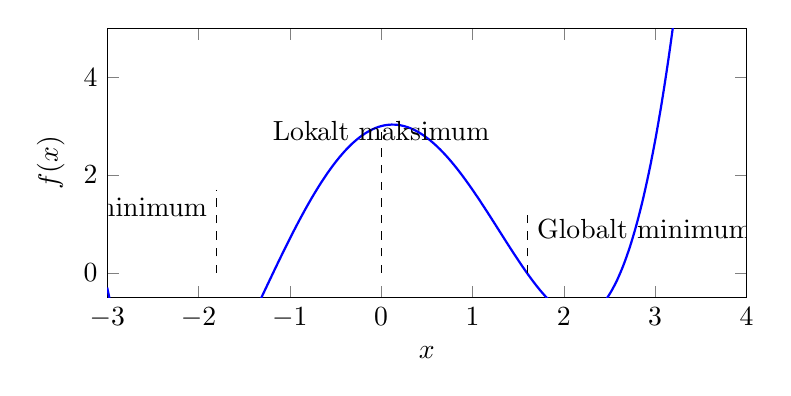
\begin{tikzpicture}
		\begin{axis}[
				xlabel={$x$},
				ylabel={$f(x)$},
				xmin=-3, xmax=4,
				ymin=-0.5, ymax=5,
				samples=100,
				smooth,
				domain=-3:4,
				width=0.8\textwidth,
				height=5cm
			]
			\addplot[blue, thick] {0.2*x^4-2*x^2+0.5*x+3};
			\draw[dashed] (axis cs:-1.8,0) -- (axis cs:-1.8,1.7);
			\draw[dashed] (axis cs:1.6,0) -- (axis cs:1.6,1.2);
			\draw[dashed] (axis cs:0,0) -- (axis cs:0,3);

			\node at (axis cs:-1.8,1.35) [anchor=east] {Lokalt minimum};
			\node at (axis cs:1.6,0.9) [anchor=west] {Globalt minimum};
			\node at (axis cs:0,3.3) [anchor=north] {Lokalt maksimum};
		\end{axis}
	\end{tikzpicture}
	\caption{Eksempel på en funksjon med både lokale og globale ekstremalpunkter}
	\label{fig:local_vs_global}
\end{figure}

Figur \ref{fig:local_vs_global} viser en funksjon med både lokale og globale ekstremalpunkter. I praksis er det generelt vanskelig å garantere at et funnet minimum er globalt, spesielt for ikke-konvekse funksjoner.

\subsection{Stasjonære Punkter}

For differensierbare funksjoner er et nødvendig vilkår for et lokalt minimum at gradienten er null.

\begin{definition}{Stasjonært punkt}{stationary_point}
	Et punkt \(\symbf{x}^\ast \in \R^n\) kalles et \textit{stasjonært punkt} for \(f\) hvis \(f\) er differensierbar ved \(\symbf{x}^\ast\) og
	\[
		\nabla f(\symbf{x}^\ast) = \symbf{0}
	\]
\end{definition}

Stasjonære punkter kan være:
\begin{itemize}
	\item Lokale minima
	\item Lokale maksima
	\item Sadelpunkter
\end{itemize}

For å skille mellom disse typene, bruker vi andreordens informasjon.

\subsection{Konveksitet}

Konvekse funksjoner spiller en spesiell rolle i optimering fordi lokale minima også er globale minima.

\begin{definition}{Konveks funksjon}{convex_function}
	En funksjon \(f: \R^n \to \R\) er \textit{konveks} hvis for alle \(\symbf{x}, \symbf{y} \in \R^n\) og alle \(\lambda \in [0,1]\) gjelder
	\[
		f(\lambda \symbf{x} + (1-\lambda)\symbf{y}) \leq \lambda f(\symbf{x}) + (1-\lambda)f(\symbf{y})
	\]
	Funksjonen er \textit{strengt konveks} hvis ulikheten over er streng for alle \(\symbf{x} \neq \symbf{y}\) og \(\lambda \in (0,1)\).
\end{definition}

For differensierbare funksjoner har vi følgende karakterisering:

\begin{proposition}{Karakterisering av differensierbare konvekse funksjoner}{differentiable_convex}
	La \(f: \R^n \to \R\) være en differensierbar funksjon. Da er \(f\) konveks hvis og bare hvis for alle \(\symbf{x}, \symbf{y} \in \R^n\) gjelder
	\[
		f(\symbf{y}) \geq f(\symbf{x}) + \nabla f(\symbf{x})^T (\symbf{y} - \symbf{x})
	\]
\end{proposition}

For to ganger differensierbare funksjoner har vi en enda enklere karakterisering:

\begin{proposition}{Karakterisering med Hesse-matrisen}{hessian_convex}
	La \(f: \R^n \to \R\) være to ganger kontinuerlig differensierbar. Da er \(f\) konveks hvis og bare hvis Hesse-matrisen \(\nabla^2 f(\symbf{x})\) er positiv semidefinit for alle \(\symbf{x} \in \R^n\).

	Funksjonen er strengt konveks hvis og bare hvis Hesse-matrisen er positiv definit for alle \(\symbf{x} \in \R^n\).
\end{proposition}

\section{Optimalitetskriterier}

\subsection{Førsteordens Nødvendige Betingelse}

\begin{theorem}{Førsteordens nødvendige betingelse}{first_order_necessary}
	Anta at \(f: \R^n \to \R\) er kontinuerlig differensierbar og at \(\symbf{x}^\ast\) er et lokalt minimum for \(f\). Da er \(\symbf{x}^\ast\) et stasjonært punkt, dvs.
	\[
		\nabla f(\symbf{x}^\ast) = \symbf{0}
	\]
\end{theorem}

\subsection{Andreordens Betingelser}

\begin{theorem}{Andreordens nødvendige betingelse}{second_order_necessary}
	Anta at \(f: \R^n \to \R\) er to ganger kontinuerlig differensierbar og at \(\symbf{x}^\ast\) er et lokalt minimum for \(f\). Da er Hesse-matrisen \(\nabla^2 f(\symbf{x}^\ast)\) positiv semidefinit.
\end{theorem}

\begin{theorem}{Andreordens tilstrekkelig betingelse}{second_order_sufficient}
	Anta at \(f: \R^n \to \R\) er to ganger kontinuerlig differensierbar, \(\nabla f(\symbf{x}^\ast) = \symbf{0}\) og Hesse-matrisen \(\nabla^2 f(\symbf{x}^\ast)\) er positiv definit. Da er \(\symbf{x}^\ast\) et strengt lokalt minimum for \(f\).
\end{theorem}

\section{Konvergens og Konvergenshastighet \texorpdfstring{\(\symbf{x}_k \to \symbf{x}^\ast\)}{x\_k to x\_ast}}
\label{sec:convergence}

I studiet av numeriske metoder for ubetinget optimering er det viktig å forstå både om og hvor raskt metodene konvergerer. Vi definerer ulike typer konvergensrater:

\begin{definition}{Konvergensrater}{convergence_rates}
	Anta at sekvensen \(\{\symbf{x}_k\}\) konvergerer mot \(\symbf{x}^\ast\). Vi sier at konvergensen er:
	\begin{itemize}
		\item \textbf{Lineær} hvis det finnes en konstant \(r \in (0,1)\) slik at
		      \[
			      \lim_{k \to \infty} \frac{\|\symbf{x}_{k+1} - \symbf{x}^\ast\|}{\|\symbf{x}_k - \symbf{x}^\ast\|} = r
		      \]

		\item \textbf{Superlineær} hvis
		      \[
			      \lim_{k \to \infty} \frac{\|\symbf{x}_{k+1} - \symbf{x}^\ast\|}{\|\symbf{x}_k - \symbf{x}^\ast\|} = 0
		      \]

		\item \textbf{Kvadratisk} hvis det finnes en konstant \(M > 0\) slik at
		      \[
			      \lim_{k \to \infty} \frac{\|\symbf{x}_{k+1} - \symbf{x}^\ast\|}{\|\symbf{x}_k - \symbf{x}^\ast\|^2} = M
		      \]
	\end{itemize}
\end{definition}

Kvadratisk konvergens betyr i praksis at antall korrekte sifre omtrent dobles i hver iterasjon, mens lineær konvergens betyr at antall korrekte sifre øker med en konstant for hver iterasjon.

\begin{figure}[h]
	\centering
	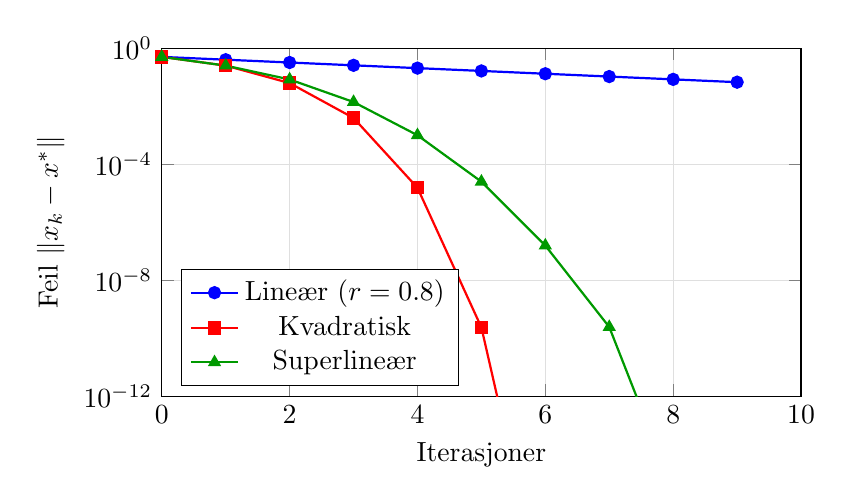
\begin{tikzpicture}
		\begin{semilogyaxis}[
				xlabel={Iterasjoner},
				ylabel={Feil $\|\symbf{x}_k - \symbf{x}^\ast\|$},
				xmin=0, xmax=10,
				ymin=1e-12, ymax=1,
				width=0.8\textwidth,
				height=6cm,
				legend pos=south west,
				grid=both,
				minor grid style={gray!25},
				major grid style={gray!25}
			]
			\addplot[blue, thick, mark=*] coordinates {
					(0, 0.5)
					(1, 0.4)
					(2, 0.32)
					(3, 0.256)
					(4, 0.2048)
					(5, 0.16384)
					(6, 0.131072)
					(7, 0.1048576)
					(8, 0.08388608)
					(9, 0.067108864)
				};
			\addlegendentry{Lineær ($r=0.8$)}

			\addplot[red, thick, mark=square*] coordinates {
					(0, 0.5)
					(1, 0.25)
					(2, 0.0625)
					(3, 0.00390625)
					(4, 1.52588e-5)
					(5, 2.32831e-10)
					(6, 5.42101e-20)
					(7, 2.93873e-39)
					(8, 8.63617e-78)
					(9, 7.45832e-155)
				};
			\addlegendentry{Kvadratisk}

			\addplot[green!60!black, thick, mark=triangle*] coordinates {
					(0, 0.5)
					(1, 0.25)
					(2, 0.0833333)
					(3, 0.0138889)
					(4, 0.000992063)
					(5, 2.48016e-5)
					(6, 1.55009e-7)
					(7, 2.40637e-10)
					(8, 5.79065e-16)
					(9, 3.35458e-27)
				};
			\addlegendentry{Superlineær}

		\end{semilogyaxis}
	\end{tikzpicture}
	\caption{Sammenligning av konvergensrater: lineær, superlineær og kvadratisk konvergens}
	\label{fig:convergence_rates}
\end{figure}

Figur \ref{fig:convergence_rates} illustrerer ulike konvergensrater. Bemerk at en logaritmisk skala brukes på y-aksen for å bedre visualisere de dramatiske forskjellene i konvergenshastighet.

I de påfølgende kapitler vil vi studere numeriske metoder for å løse ubetingede optimeringsproblemer og analysere deres konvergensegenskaper.

\chapter{Gradient metoder}
\label{chap:gradient_based_methods}
Gradientbaserte metoder er en klasse av numeriske algoritmer som benytter gradienten til objektfunksjonen for å finne minimum eller maksimum.
Disse metodene kan kategoriseres etter hvilken ordens derivert de bruker:

\begin{itemize}
	\item \textbf{Førsteordens metoder}: Bruker bare gradientinformasjon (f.eks. Steepest Descent)
	\item \textbf{Andreordens metoder}: Bruker både gradient og Hesse-matrise (f.eks. Newtons metode)
\end{itemize}

Man klassifiserer også gradientbaserte metoder i to hovedkategorier, \emph{linjesøkmetoder} og \emph{trust region-metoder}.
I linjesøkmetoder bestemmer vi først søkeretningen, deretter hvor langt vi skal gå i den retningen.
I trust region-metoder bestemmer vi først hvor langt vi kan gå (trust region-radiusen), deretter bestemmer vi både retning og steglengde samtidig.

\begin{forest}
	for tree={
	align=center,
	parent anchor=south,
	child anchor=north
	}
	[Gradientbaserte\\ metoder
		[Førsteordens\\ metoder
				[Steepest\\ Descent]
				[Konjugert\\ Gradient]
		]
		[Andreordens\\ metoder
				[Newtons\\ metode]
				[Quasi-Newton\\ metoder]
		]
	]
\end{forest}

\medskip
Både første- og andreordens metoder kan implementeres med enten linjesøk eller trust region strategier.
\section{Steepest Descent}\label{sec:steepest_descent}
Steepest Descent en en enkel metode for å minimere \(f: \mathbb{R}^n \to \mathbb{R}\) ved å følge den bratteste nedstigningsretningen \( \symbf{d}_k = -\nabla f(\symbf{x}_k)\) fra et gitt punkt \( \symbf{x}_k \).
\begin{definition}{Steepest Descent}{steepest_descent}
	Steepest Descent-algoritmen oppdaterer iterasjonen \( \symbf{x}_k \) ved å ta et skritt i retning av den negative gradienten:
	\[
		\symbf{x}_{k+1} = \symbf{x}_k + \alpha_k \symbf{d}_k,
	\]
	hvor \( \alpha_k > 0 \) er skrittlengden og \( \symbf{d}_k = -\nabla f(\symbf{x}_k) \) er nedstigningsretningen.
	\medskip
	Steepest Descent-algoritmen kan skrives som:
	\begin{align*}
		\symbf{x}_{k+1} & = \symbf{x}_k + \alpha_k \symbf{d}_k, \\
		\symbf{d}_k     & = -\nabla f(\symbf{x}_k).
	\end{align*}

\end{definition}

\begin{equation}
	\symbf{d}_k = -\nabla f(\symbf{x}_k),
\end{equation}
hvor \(\symbf{d}_k\) er nedstigningsretningen ved iterasjon \(k\).
\subsection{Steepest Descent Algoritme}
\begin{algorithm}[H]
	\SetAlgoLined
	\KwIn{Startpunkt \( \symbf{x}_0 \), toleranse \( \epsilon \), maks antall iterasjoner \( K \)}
	\KwOut{Omtrentelig løsning \( \symbf{x}^\ast \)}
	\For{\( k = 0, 1, 2, \ldots, K\)}{
		\(\symbf{d}_k = -\nabla f(\symbf{x}_k)\)\;
		Finn skrittlengde \(\alpha_k\) (f.eks.\ ved linjesøk-metode)\;
		\(\symbf{x}_{k+1} = \symbf{x}_k + \alpha_k \symbf{d}_k\)\;
		\If{\(\|\nabla f(\symbf{x}_{k+1})\| < \epsilon\)}{
			\Return \(\symbf{x}_{k+1}\)\;
		}
	}
	\caption{Steepest Descent}
	\label{alg:steepest_descent}
\end{algorithm}

\subsection{Konvergens av Steepest Descent}
Anta ett ideelt tilfelle der \(f\) er en kvadratisk funksjon, med en positiv definit og symmetrisk Hesse-matrise \(Q\), hvor objektfunksjonen er kvadratisk og linjesøkene er eksakte.
\begin{align*}
	f(\symbf{x})        & = \frac{1}{2} \symbf{x}^T Q \symbf{x} - \symbf{b}^T \symbf{x} \\
	\nabla f(\symbf{x}) & = Q \symbf{x} - \symbf{b}
\end{align*}\label{eq:quadratic_function}

hvor det minste punkt \(\symbf{x}^\ast\) er en unik løsning av
\[
	Q \symbf{x}^\ast = \symbf{b}.
\]
Da kan vi finne den beste steglengden \(\alpha_k\) som minimerer \(f(\symbf{x}_k - \alpha \nabla f(\symbf{x}_k))\) ved å derivere den med hensyn til \(\alpha\) og sette den lik null:
\begin{align*}
	f(\symbf{x}_k - \alpha \nabla f(\symbf{x}_k)) & = \frac{1}{2} (\symbf{x}_k - \alpha \nabla f(\symbf{x}_k))^T Q (\symbf{x}_k - \alpha \nabla f(\symbf{x}_k)) - \symbf{b}^T (\symbf{x}_k - \alpha \nabla f(\symbf{x}_k)), \\
	\frac{\partial f}{\partial \alpha}            & = -\nabla f(\symbf{x}_k)^T Q \symbf{x}_k + \alpha \nabla f(\symbf{x}_k)^T Q \nabla f(\symbf{x}_k) + \nabla f(\symbf{x}_k)^T \nabla f(\symbf{x}_k).
\end{align*}
Med å løse \(\frac{\partial f}{\partial \alpha} = 0\) for \(\alpha_k\) får vi:

\[
	\alpha_k = \frac{\nabla f_k^\top \nabla f_k}{\nabla f_k^\top Q \nabla f_k}
\]

Det gir oss den eksakte optimale steglengden \(\alpha_k\) for Steepest Descent-algoritmen.
\begin{equation*}
	\symbf{x}_{k+1} = \symbf{x}_k - \alpha_k \nabla f(\symbf{x}_k) = \symbf{x}_k - \left(\frac{\nabla f_k^\top \nabla f_k}{\nabla f_k^\top Q \nabla f_k}\right) \nabla f_k
\end{equation*}\label{eq:steepest_descent_update}
\subsection{Konvergenshastighet for Steepest Descent}
For å analysere konvergenshastigheten til Steepest Descent-algoritmen, vil vi undersøke hvordan feilen reduseres for hver iterasjon. Vi fokuserer først på det kvadratiske tilfellet med en positiv definit Hesse-matrise $Q$.

La oss definere feilen ved iterasjon $k$ som $\symbf{e}_k = \symbf{x}_k - \symbf{x}^\ast$, der $\symbf{x}^\ast$ er den eksakte løsningen. For en kvadratisk funksjon gjelder følgende forhold:
\[
	\frac{1}{2} \|\symbf{e}_k\|_Q^2 = \frac{1}{2} \|\symbf{x}_k - \symbf{x}^\ast\|_Q^2 = f(\symbf{x}_k) - f(\symbf{x}^\ast).
\]

Med eksakt linjesøk kan vi, basert på oppdateringsformelen~\eqref{eq:steepest_descent_update}, vise at feilen avtar lineært:
\[
	\|\symbf{e}_{k+1}\|_Q^2 = (1 - C) \|\symbf{e}_k\|_Q^2,
\]
hvor reduksjonsfaktoren $C$ er gitt ved:
\[
	C = \frac{[\nabla f_k^\top \nabla f_k]^2}{(\nabla f_k^\top Q \nabla f_k)(\nabla f_k^\top Q^{-1} \nabla f_k)}.
\]

Dette uttrykket kan være komplisert å beregne direkte, men vi kan etablere en øvre grense ved hjelp av kondisjonstallet til $Q$:

\begin{theorem}{Konvergenshastighet for Steepest Descent}{steepest_descent_convergence}
	Når Steepest Descent-metoden med eksakte linjesøk anvendes på en sterkt konveks kvadratisk funksjon~\eqref{eq:quadratic_function}, er konvergenshastigheten begrenset av:
	\[
		\norm{\symbf{x}_{k+1} - \symbf{x}^\ast}_Q^2 \leq \left(\frac{\kappa - 1}{\kappa + 1}\right)^2 \norm{\symbf{x}_k - \symbf{x}^\ast}_Q^2,
	\]
	hvor $\kappa = \frac{\lambda_n}{\lambda_1}$ er kondisjonstallet til $Q$, med $0 < \lambda_1 \leq \lambda_2 \leq \cdots \leq \lambda_n$ som egenverdiene til $Q$.
\end{theorem}

Dette resultatet viser at konvergenshastigheten til Steepest Descent i stor grad avhenger av kondisjonstallet $\kappa$. Når $\kappa$ er stort (dårlig kondisjonert problem), nærmer faktoren $\frac{\kappa - 1}{\kappa + 1}$ seg 1, hvilket resulterer i svært langsom konvergens.

For den generelle, ikke-kvadratiske situasjonen kan vi forvente lignende lineær konvergensatferd nær løsningen, men med konstanten bestemt av kondisjonstallet til Hesse-matrisen ved løsningspunktet.

En detaljert utledning av dette resultatet finnes i \cite{luenberger1984linear}.

\subsection{Konvergens ved generelle funksjoner}
For generelle, ikke-kvadratiske funksjoner \(f : \mathbb{R}^n \to \mathbb{R}\), gjelder fremdeles en lineær konvergensrate for Steepest Descent-metoden dersom \(f\) er to ganger kontinuerlig deriverbar og linjesøket er eksakt.
Men man kan fortsatt vise at konvergenshastigheten i nærheten av en løsning \(x^\ast\) fortsatt begrenses av kondisjonstallet til Hesse-matrisen.

\begin{theorem}{Asymptotisk konvergens av Steepest Descent}{steepest_descent_general}
	Anta at \(f : \mathbb{R}^n \to \mathbb{R}\) er to ganger kontinuerlig deriverbar og at iteratene \(\symbf{x}_k\) generert av Steepest Descent med eksakt linjesøk konvergerer til et punkt \(x^\ast\), hvor Hesse-matrisen \(\nabla^2 f(x^\ast)\) er positiv definit.

	La \(\lambda_1 \leq \lambda_2 \leq \cdots \leq \lambda_n\) være egenverdiene til \(\nabla^2 f(x^\ast)\). Da finnes det en konstant \(r \in \left( \frac{\lambda_n - \lambda_1}{\lambda_n + \lambda_1}, 1 \right)\) slik at
	\[
		f(x_{k+1}) - f(x^\ast) \leq r^2 \left[ f(x_k) - f(x^\ast) \right]
	\]
	for alle tilstrekkelig store \(k\).
\end{theorem}

Dette viser at metoden har \emph{lineær konvergens}, men at konvergensfaktoren \(r^2\) nærmer seg 1 når kondisjonstallet \(\kappa = \lambda_n / \lambda_1\) blir stort. Dette innebærer at selv under ideelle forhold (eksakt linjesøk og glatt funksjon), kan Steepest Descent konvergere ekstremt langsomt. For eksempel, hvis \(\kappa = 800\) og startverdien er \(f(x_1) = 1\), kan man etter 1000 iterasjoner fortsatt ha

\section{Newtons Metode}
\label{sec:newtons_method}
Newtons metode er en iterativ metode for å finne stasjonære punkter (typisk minima eller maxima) av glatt funksjoner.
\[
	\mathbf{x}_{k+1} = \mathbf{x}_k - [\nabla^2 f(\mathbf{x}_k)]^{-1} \nabla f(\mathbf{x}_k) = \mathbf{x}_k - \alpha_k \mathbf{d}_k
\]\label{eq:newtons_method}

Den bruker 2. Ordens Taylor-approksimasjoner av objektfunksjonen, og bruker både gradienten og Hesse-matrisen $H$ til å finne en retning $\symbf{d}_k$ for å oppdatere iterasjonen $\symbf{x}_k$.

\[
	\symbf{d}_k = -[\nabla^2 f(\symbf{x}_k)]^{-1} \nabla f(\symbf{x}_k) = -\symbf{H}^{-1} \nabla f(\symbf{x}_k)
\]

Ulempen er at metoden krever at man finner Hesse-matrisen $H$, og regner ut dens inverse $H^{-1}$, noe som kan være kostbart i høyere dimensjoner.

Under visse regularitetsforutsetninger kan metoden konvergere med kvadratisk hastighet $\norm{e}_{k+1} \leq C \norm{e_k}^2$, noe som gjør den vesentlig mer effektiv enn førsteordens metoder i nærhet av løsningen.
Med regularitetsforutsetninger menes at objektfunksjonen $f$ er to ganger kontinuerlig deriverbar, og at Hesse-matrisen $\nabla^2 f(x^\ast)$ ved løsningen $x^\ast$ er positiv definit.
Disse forutsetningene sikrer at metoden kan utnytte kurvaturinformasjonen i $f$ for raskere konvergens.

\[
	\norm{\symbf{e}_{k+1}} \leq C \norm{\symbf{e}_k}^2 \approx \mathcal{O}(\norm{\symbf{e}_k}^2)
\]

\subsection{Newtons Metode Algoritme}
Skrittlengden \(\alpha_k\) kan bestemmes ved linjesøk, eller andre metoder for å minimere \(f(\symbf{x}_k + \alpha \symbf{d}_k)\) i retning av \(\symbf{d}_k\).

\begin{algorithm}[H]
	\SetAlgoLined
	\KwIn{Startpunkt \( \symbf{x}_0 \), tol. \( \epsilon > 0 \), maks iter. \( K_{max} \)}
	\KwOut{Løsning \( \approx \symbf{x}^\ast \)}
	Start Skritt \(\alpha_0 = 1\)\;
	\For{\( k = 0, 1, 2, \ldots, K_{max}\)}{
	\(\symbf{d}_k = -[\nabla^2 f(\symbf{x}_k)]^{-1}\,\nabla f(\symbf{x}_k)\)\;
	Finn Ny Skritt \(\alpha_k\) (f.eks.\ ved linjesøk-metoder)\;
	\(\symbf{x}_{k+1} = \symbf{x}_k + \alpha_k \symbf{d}_k\)\;
	\If{\(\|\nabla f(\symbf{x}_{k+1})\| < \epsilon\)}{
		\Return \(\symbf{x}_{k+1}\)\;
	}
	}
	\caption{Newtons metode}
\end{algorithm}

\subsection{Konvergens av Newtons Metode}
Newtons metode kan konvergere lokalt kvadratisk under visse forutsetninger.
La \( f : \mathbb{R}^n \to \mathbb{R} \) være to ganger kontinuerlig deriverbar. Anta at:

\begin{enumerate}
	\item Det finnes et \(\symbf{x}^\ast\) slik at \(\nabla f(\symbf{x}^\ast) = 0\).
	\item Hesse-matrisen \(\nabla^2 f(\symbf{x}^\ast)\) er regulær (invertibel).
	\item \(\nabla^2 f\) er Lipschitz-kontinuerlig i et nabolag rundt \(\symbf{x}^\ast\); dvs.\ det finnes \( L > 0 \) slik at
	      \[
		      \| \nabla^2 f(\symbf{x}) - \nabla^2 f(\symbf{y}) \|
		      \;\le\;
		      L\,\|\symbf{x} - \symbf{y}\|,
	      \]
	      for alle \(\symbf{x}, \symbf{y}\) i dette nabolaget.
\end{enumerate}

Da kan man vise at for en startverdi \(\symbf{x}_0\) nær \(\symbf{x}^\ast\), vil Newtons metode konvergere kvadratisk mot \(\symbf{x}^\ast\).
Beviset forutsetter at startverdien \(\symbf{x}_0\) er tilstrekkelig nær \(\symbf{x}^\ast\). I praksis benyttes ofte modifikasjoner, som for eksempel \textit{dempet Newton} (med linjesøk), for å sikre global konvergens før man oppnår den raske, lokale konvergensfasen.
\begin{proof}{}{}
	La \(\symbf{e}_k = \symbf{x}_k - \symbf{x}^\ast\) være feilen ved iterasjon \(k\).
	Ved Taylor-utvidelse av gradienten får vi:
	\[
		\nabla f(\symbf{x}_k)
		= \nabla^2 f(\symbf{x}^\ast)\,(\symbf{x}_k - \symbf{x}^\ast) + r(\symbf{x}_k),
	\]
	hvor \(\|r(\symbf{x}_k)\|\) er \(\mathcal{O}(\|\symbf{e}_k\|^2)\). Newtons oppdateringsregel er
	\[
		\symbf{x}_{k+1}
		= \symbf{x}_k
		- [\nabla^2 f(\symbf{x}_k)]^{-1}\,\nabla f(\symbf{x}_k).
	\]
	I et lite nabolag av \(\symbf{x}^\ast\) kan vi anta at
	\(\nabla^2 f(\symbf{x}_k)\approx \nabla^2 f(\symbf{x}^\ast)\), slik at
	\[
		\symbf{e}_{k+1}
		\;=\; \symbf{x}_{k+1} - \symbf{x}^\ast
		\;\approx\;
		-[\nabla^2 f(\symbf{x}^\ast)]^{-1}\,r(\symbf{x}_k).
	\]
	Dermed blir
	\[
		\|\symbf{e}_{k+1}\| \lesssim \|[\nabla^2 f(\symbf{x}^\ast)]^{-1}\| \|r(\symbf{x}_k)\| \le C \|\symbf{e}_k\|^2
	\]
	for en konstant \(C>0\). Dette illustrerer \textit{kvadratisk konvergens} når \(\symbf{x}_0\) er nært \(\symbf{x}^\ast\).
\end{proof}

\subsection{Egenskaper}
\begin{itemize}
	\item \textbf{Kvadratisk konvergens}: Under gitte forutsetninger dobles antall riktige sifre omtrent for hver iterasjon.
	\item \textbf{Krever andreordens deriverbarhet}: \(\nabla^2 f(\symbf{x})\) må eksistere og være invertibel.
	\item \textbf{Beregning kan være kostbar}: Å beregne og invertere \(\nabla^2 f(\symbf{x})\) er dyrt, spesielt i store dimensjoner.
	\item \textbf{Global vs.\ lokal konvergens}: Metoden garanterer ikke nødvendigvis global konvergens uten videre tiltak.
\end{itemize}

\subsection{Varianter av Newtons metode}
\begin{itemize}
	\item \textbf{Dempet Newtons metode}: Benytter en skrittlengde \(\alpha_k\) (linjesøk) for å unngå for store steg.
	\item \textbf{Kvasi-Newton-metoder}: Reduserer kostnader ved å approksimere Hesse-matrisen (f.eks.\ BFGS, DFP).
\end{itemize}

\section{Konjugert Gradientmetoden}
\label{sec:conjugate_gradient}

Konjugert Gradient (CG) metoden er en effektiv iterativ algoritme for å løse lineære ligningssystemer og optimere kvadratiske funksjoner. Den er spesielt nyttig for store, men sparse systemer.

\subsection{Grunnleggende Konsept}
CG-metoden genererer en sekvens av retninger som er konjugerte med hensyn til en symmetrisk, positiv definit matrise. For en kvadratisk funksjon:
\[
	f(\symbf{x}) = \frac{1}{2}\symbf{x}^T\symbf{A}\symbf{x} - \symbf{b}^T\symbf{x} + c,
\]
hvor \(\symbf{A}\) er symmetrisk, positiv definit, søker CG-metoden å løse \(\nabla f(\symbf{x}) = \symbf{A}\symbf{x} - \symbf{b} = \symbf{0}\).

\subsection{CG-algoritme}

\begin{algorithm}[H]
	\SetAlgoLined
	\KwIn{Startpunkt \(\symbf{x}_0\), toleranse \(\epsilon > 0\)}
	\KwOut{Omtrentelig løsning \(\symbf{x}^\ast\)}
	\(\symbf{r}_0 \gets \symbf{b} - \symbf{A}\symbf{x}_0\) \tcc*{Residual}
	\(\symbf{p}_0 \gets \symbf{r}_0\) \tcc*{Første søkeretning}
	\For{\(k = 0, 1, 2, \ldots\)}{
		\If{\(\|\symbf{r}_k\| < \epsilon\)}{
			\Return \(\symbf{x}_k\) \tcc*{Konvergens oppnådd}
		}
		\(\alpha_k \gets \frac{\symbf{r}_k^T\symbf{r}_k}{\symbf{p}_k^T\symbf{A}\symbf{p}_k}\) \tcc*{Optimal skrittlengde}
		\(\symbf{x}_{k+1} \gets \symbf{x}_k + \alpha_k\symbf{p}_k\) \tcc*{Oppdater løsning}
		\(\symbf{r}_{k+1} \gets \symbf{r}_k - \alpha_k\symbf{A}\symbf{p}_k\) \tcc*{Oppdater residual}
		\(\beta_{k+1} \gets \frac{\symbf{r}_{k+1}^T\symbf{r}_{k+1}}{\symbf{r}_k^T\symbf{r}_k}\) \tcc*{Konjugasjonsparameter}
		\(\symbf{p}_{k+1} \gets \symbf{r}_{k+1} + \beta_{k+1}\symbf{p}_k\) \tcc*{Ny søkeretning}
	}
	\caption{Konjugert Gradient Metode (CG)}
\end{algorithm}

\subsection{Ikke-lineær Konjugert Gradient Metode (Non-Linear CG)}

For generelle ikke-lineære funksjoner tilpasses algoritmen:

\begin{algorithm}[H]
	\SetAlgoLined
	\KwIn{Startpunkt \(\symbf{x}_0\), toleranse \(\epsilon > 0\)}
	\KwOut{Omtrentelig løsning \(\symbf{x}^\ast\)}
	\(\symbf{g}_0 \gets \nabla f(\symbf{x}_0)\) \tcc*{Gradient}
	\(\symbf{p}_0 \gets -\symbf{g}_0\) \tcc*{Første søkeretning}
	\For{\(k = 0, 1, 2, \ldots\)}{
		\If{\(\|\symbf{g}_k\| < \epsilon\)}{
			\Return \(\symbf{x}_k\) \tcc*{Konvergens oppnådd}
		}
		Finn \(\alpha_k\) ved linjesøk som minimerer \(f(\symbf{x}_k + \alpha\symbf{p}_k)\) \;
		\(\symbf{x}_{k+1} \gets \symbf{x}_k + \alpha_k\symbf{p}_k\) \tcc*{Oppdater løsning}
		\(\symbf{g}_{k+1} \gets \nabla f(\symbf{x}_{k+1})\) \tcc*{Ny gradient}
		Beregn \(\beta_{k+1}\) \tcc*{f.eks. FR eller PR}\;
		\(\symbf{p}_{k+1} \gets -\symbf{g}_{k+1} + \beta_{k+1}\symbf{p}_k\) \tcc*{Ny søkeretning}
	}
	\caption{Ikke-lineær Konjugert Gradient Metode (Non-Linear CG)}
\end{algorithm}

\(\beta_{k+1}\) er konjugasjonsparameteren som bestemmer hvordan den nye søkeretningen \(\symbf{p}_{k+1}\) kombinerer den nåværende gradienten \(\symbf{g}_{k+1}\) med den forrige søkeretningen \(\symbf{p}_k\).
Intuitivt er egentlig \(\beta_{k+1}\) bare en vekt som bestemmer hvor mye av den forrige retningen \(\symbf{p}_k\) som skal beholdes i den nye retningen \(\symbf{p}_{k+1}\).

\subsection{Valg av \texorpdfstring{\(\beta\)}{beta}-parameter}
Det finnes flere metoder for å velge \(\beta_{k+1}\) i den ikke-lineære konjugerte gradientmetoden.

\subsubsection{Fletcher-Reeves (FR)}
Fletcher-Reeves oppdaterer \(\beta_{k+1}\) basert på forholdet mellom normene til gradientene i to påfølgende iterasjoner.
Dette sikrer at søkeretningene forblir konjugerte med hensyn til Hessian-matrisen for kvadratiske funksjoner.

\begin{definition}{Fletcher--Reeves}{fletcher_reeves}
	\[
		\beta_{k+1}^{FR} = \frac{\symbf{g}_{k+1}^T\symbf{g}_{k+1}}{\symbf{g}_k^T\symbf{g}_k} \tag{FR}
	\]
\end{definition}

\subsubsection{Polak--Ribière (PR)}
Polak--Ribière oppdaterer \(\beta_{k+1}\) basert på både normene til gradientene og forskjellen mellom gradientene i to påfølgende iterasjoner. Dette gir en mer dynamisk oppdatering sammenlignet med Fletcher--Reeves.
\begin{definition}{Polak-Ribière}{polak_ribiere}
	\[
		\beta_{k+1}^{PR} = \frac{\symbf{g}_{k+1}^T(\symbf{g}_{k+1}-\symbf{g}_k)}{\symbf{g}_k^T\symbf{g}_k} \tag{PR}
	\]
\end{definition}


\begin{remark}{Håndtering av negativ \(\beta_{k+1}^{PR}\)}{}
	Denne metoden kan gi raskere konvergens i praksis, men kan også føre til ustabilitet hvis \(\beta_{k+1}^{PR}\) blir negativ.
	I slike tilfeller kan \(\beta_{k+1}^{PR}\) settes til null for å sikre at algoritmen fortsatt fungerer som en gradientmetode.
\end{remark}

\subsubsection{Hestenes--Stiefel (HS)}
Hestenes--Stiefel oppdaterer \(\beta_{k+1}\) ved å bruke forholdet mellom gradientforskjellen og søkeretningen.
\begin{definition}{Hestenes--Stiefel}{hestenes_stiefel}
	\[
		\beta_{k+1}^{HS} = \frac{\symbf{g}_{k+1}^T(\symbf{g}_{k+1} - \symbf{g}_k)}{\symbf{p}_k^T(\symbf{g}_{k+1} - \symbf{g}_k)} \tag{HS}
	\]
\end{definition}
Hestenes--Stiefel-metoden kan være mer effektiv enn både Fletcher--Reeves og Polak--Ribière i visse tilfeller, spesielt når gradientforskjellene \(\symbf{g}_{k+1} - \symbf{g}_k\) er små, og søkeretningene \(\symbf{p}_k\) er godt tilpasset problemets kurvatur.
Dette skyldes at Hestenes--Stiefel-formelen tar hensyn til både gradientendringer og søkeretningens geometri, noe som kan gi en mer stabil oppdatering av \(\beta_{k+1}\).

\begin{remark}{Ustabilitet i Hestenes--Stiefel-metoden}{}
	En potensiell ulempe med Hestenes--Stiefel-metoden er at den kan bli ustabil hvis nevneren \(\symbf{p}_k^T(\symbf{g}_{k+1} - \symbf{g}_k)\) blir svært liten. For å unngå dette kan man bruke en modifisert versjon der \(\beta_{k+1}\) settes til null når ustabilitet oppdages.
\end{remark}

\begin{example}{}{}
	Anta at vi ønsker å minimere en kvadratisk funksjon \(f(\symbf{x}) = \frac{1}{2}\symbf{x}^\top A\symbf{x} - \symbf{b}^\top \symbf{x}\), der \(A\) er symmetrisk og positiv definit.
	\ref{def:hestenes_stiefel} kan gi raskere konvergens enn Fletcher--Reeves og Polak--Ribière hvis \(A\) har et høyt kondisjonstall \(\kappa(A)\), fordi den bedre utnytter informasjonen om gradientendringene.
\end{example}

Likevel kan den føre til ustabilitet hvis nevneren blir svært liten.
For å unngå dette kan man sette \(\beta_{k+1}^{HS} = 0\) når det er nødvendig for å opprettholde stabiliteten.

\subsection{Egenskaper}
\begin{itemize}
	\item \textbf{Rask konvergens for kvadratiske funksjoner:}
	      For kvadratiske funksjoner konvergerer metoden på maksimalt \(n\) iterasjoner.
	\item \textbf{Minneeffektivitet:}
	      Metoden lagrer kun et begrenset antall vektorer, noe som gjør den godt egnet for store problemer.
	\item \textbf{Numerisk stabilitet:}
	      Den er robust mot avrundingsfeil og opprettholder numerisk stabilitet, spesielt når periodiske omstarter benyttes.\footnote{Periodiske omstarter innebærer å tilbakestille algoritmen med jevne mellomrom for å reinitialisere retningene og sikre at de forblir ortogonale. Denne teknikken bidrar til å redusere akkumulerte beregningsfeil og opprettholder algoritmens effektivitet.}
	\item \textbf{Prekondisjonering:}
	      Metodens ytelse kan forbedres ytterligere ved å bruke en prekondisjonerer \(M\), som transformerer problemet for å akselerere konvergensen.
\end{itemize}

\subsection{Prekondisjonering}
Konvergenshastigheten kan forbedres ved å bruke en prekondisjonerer \(\symbf{M}\) som approksimerer \(\symbf{A}\) på en inverterbar måte. Den prekondisjonerte algoritmen løser det transformerte systemet:
\[
	\symbf{M}^{-1}\symbf{A}\symbf{x} = \symbf{M}^{-1}\symbf{b}.
\]
Dette reduserer kondisjonstallet \(\kappa(\symbf{M}^{-1}\symbf{A})\) og akselererer konvergensen.

\section{Quasi-Newton Metoder}
\label{sec:quasi_newton}

Quasi-Newton-metoder er en klasse av optimeringsalgoritmer utviklet for å løse ikke-lineære optimeringsproblemer. De bygger på ideene bak Newtons metode, men er spesielt nyttige når Hesse-matrisen \( \nabla^2 f(\symbf{x}) \) er vanskelig å beregne eller invertere.

Ettersom eksplisitt inversjon av Hesse-matrisen krever \( \mathcal{O}(n^2) \) lagring og \( \mathcal{O}(n^3) \) regneoperasjoner, blir Newtons metode ofte upraktisk i høyere dimensjoner.
Quasi-Newton-metoder unngår dette ved å iterativt lage en approksimasjon av Hesse-matrisen, eller dens invers, basert på gradientinformasjon fra tidligere iterasjoner.

Søkeretningen defineres da som
\[
	\symbf{p}_k = -B_k^{-1} \nabla f(\symbf{x}_k),
\]
der \( B_k \) er en symmetrisk og positivt definit matrise som approksimerer \( \nabla^2 f(\symbf{x}_k) \). Steglengden \( \alpha_k \) velges vanligvis gjennom linjesøk som tilfredsstiller Wolfe- eller sterke Wolfe-betingelser.

\subsection{Motivasjon}
Newtons metode krever eksplisitt beregning og inversjon av Hesse-matrisen \( \nabla^2 f(\symbf{x}) \) i hver iterasjon, noe som er kostbart i høyere dimensjoner.

Quasi-Newton-metoder reduserer denne kostnaden ved å:
\begin{itemize}
	\item Lage en iterativ approksimasjon av Hesse-matrisen (eller dens invers),
	\item Oppdatere denne approksimasjonen ved hjelp av gradientforskjeller fra tidligere iterasjoner,
	\item Unngå eksplisitt inversjon gjennom spesifikke oppdateringsformler.
\end{itemize}

\subsection{Algoritme for Quasi-Newton metoder}

\begin{algorithm}[H]
	\DontPrintSemicolon
	\KwIn{Startpunkt \( \mathbf{x}_0 \in \mathbb{R}^n \), toleranse \( \varepsilon > 0 \), initial matrise \( \mathbf{B}_0 \succ 0 \)}
	\KwOut{Omtrentlig løsning \( \mathbf{x}^\ast \)}

	\textbf{Initialiser:} \( k \gets 0 \)\;
	\While{\( \| \nabla f(\mathbf{x}_k) \| > \varepsilon \)}{
	Beregn søkeretning: \( \mathbf{p}_k = -\mathbf{B}_k^{-1} \nabla f(\mathbf{x}_k) \)\;

	Velg steglengde \( \alpha_k > 0 \) ved linjesøk (f.eks. Wolfe-betingelser)\;

	Oppdater iterasjon: \( \mathbf{x}_{k+1} = \mathbf{x}_k + \alpha_k \mathbf{p}_k \)\;

	Definer: \( \mathbf{s}_k = \mathbf{x}_{k+1} - \mathbf{x}_k \), \quad
	\( \mathbf{y}_k = \nabla f(\mathbf{x}_{k+1}) - \nabla f(\mathbf{x}_k) \)\;

	Oppdater \( \mathbf{B}_k \to \mathbf{B}_{k+1} \) ved bruk av f.eks. BFGS-oppdatering:\;
	\Indp
	\( \mathbf{B}_{k+1} = \mathbf{B}_k
	- \frac{\mathbf{B}_k \mathbf{s}_k \mathbf{s}_k^\top \mathbf{B}_k}{\mathbf{s}_k^\top \mathbf{B}_k \mathbf{s}_k}
	+ \frac{\mathbf{y}_k \mathbf{y}_k^\top}{\mathbf{y}_k^\top \mathbf{s}_k} \)\;
	\Indm

	\( k \gets k + 1 \)\;
	}

	\Return \( \mathbf{x}_k \)\;
	\caption{Quasi-Newton Metode}
	\label{alg:quasi_newton}
\end{algorithm}

\subsection{Sekantligningen}
For å oppdatere Hesse-approksimasjonen, må vi løse sekantligningen:
\[
	\symbf{B}_{k+1}\symbf{s}_k = \symbf{y}_k,
\]
Dette er en viktig del av Quasi-Newton-metodene, da den gir oss en måte å oppdatere Hesse-approksimasjonen på uten å måtte beregne den eksakte Hesse-matrisen.

I praksis jobber vi ofte direkte med den inverse approksimasjonen av Hesse-matrisen, \(\symbf{H}_k\), i stedet for \(\symbf{B}_k\). Dette er fordi det er mer numerisk stabilt og krever mindre minne.
\[
	\symbf{H}_k \approx [\nabla^2 f(\symbf{x}_k)]^{-1} =[\symbf{B}_k^{METODE}]^{-1}
\]

\subsection{Broyden-Fletcher-Goldfarb-Shanno (BFGS) oppdatering}
BFGS er en av de mest brukte Quasi-Newton-metodene.
Den oppdaterer den inverse Hesse-approksimasjonen ved å bruke gradientinformasjon fra to påfølgende iterasjoner.

\begin{definition}{BFGS-oppdatering}{bfgs_update}

	\begin{align*}
		\symbf{B}_{k+1}^{BFGS} & = \symbf{B}_k - \frac{\symbf{B}_k\symbf{s}_k\symbf{s}_k^T\symbf{B}_k}{\symbf{s}_k^T\symbf{B}_k\symbf{s}_k} + \frac{\symbf{y}_k\symbf{y}_k^T}{\symbf{y}_k^T\symbf{s}_k}                                                                          \\
		\symbf{H}_{k+1}        & = \left(\symbf{I} - \frac{\symbf{s}_k\symbf{y}_k^T}{\symbf{y}_k^T\symbf{s}_k}\right) \symbf{H}_k \left(\symbf{I} - \frac{\symbf{y}_k\symbf{s}_k^T}{\symbf{y}_k^T\symbf{s}_k}\right) + \frac{\symbf{s}_k\symbf{s}_k^T}{\symbf{y}_k^T\symbf{s}_k}
	\end{align*}

\end{definition}

\subsection{Davidon-Fletcher-Powell (DFP) oppdatering}
DFP er en annen viktig Quasi-Newton oppdatering.

\begin{definition}{DFP-oppdatering}{dfp_update}
	\begin{align*}
		\symbf{B}_{k+1}^{DFP} = \symbf{B}_k - \frac{\symbf{B}_k\symbf{y}_k\symbf{y}_k^T\symbf{B}_k}{\symbf{y}_k^T\symbf{B}_k\symbf{y}_k} + \frac{\symbf{s}_k\symbf{s}_k^T}{\symbf{s}_k^T\symbf{y}_k} \tag{Oppdatering av Hesse-approksimasjonen} \\
		\symbf{H}_{k+1} = \symbf{H}_k - \frac{\symbf{H}_k\symbf{y}_k\symbf{y}_k^T\symbf{H}_k}{\symbf{y}_k^T\symbf{H}_k\symbf{y}_k} + \frac{\symbf{s}_k\symbf{s}_k^T}{\symbf{y}_k^T\symbf{s}_k} \tag{Oppdatering av invers Hesse-approksimasjonen}
	\end{align*}
\end{definition}

\subsection{Broydens klasse}
BFGS og DFP er spesialtilfeller av en mer generell familie av oppdateringsformler kjent som Broydens klasse.

Denne familien av metoder tillater en trade-off mellom numerisk stabilitet (BFGS) og teoretisk optimalitet (DFP).

\begin{definition}{Broydens klasse}{broydens_class}
	For en parameter $\phi \in [0,1]$, defineres Broydens klasse av oppdateringer for den inverse Hesse-approksimasjonen som:
	\[
		\symbf{H}_{k+1}^\phi = (1-\phi)\symbf{H}_{k+1}^{BFGS} + \phi\symbf{H}_{k+1}^{DFP}
	\]
	hvor $\symbf{H}_{k+1}^{BFGS}$ og $\symbf{H}_{k+1}^{DFP}$ er henholdsvis BFGS- og DFP-oppdateringene.
\end{definition}

Dette kan utvides til en eksplisitt form:

\begin{proposition}{Broydens oppdateringsformel}{broydens_update}
	Oppdateringsformelen for Broydens klasse kan skrives som:
	\[
		\symbf{H}_{k+1}^\phi = \symbf{H}_k - \frac{\symbf{H}_k\symbf{y}_k\symbf{y}_k^T\symbf{H}_k}{\symbf{y}_k^T\symbf{H}_k\symbf{y}_k} + \frac{\symbf{s}_k\symbf{s}_k^T}{\symbf{y}_k^T\symbf{s}_k} + \phi\left(\frac{\symbf{y}_k^T\symbf{H}_k\symbf{y}_k}{\symbf{y}_k^T\symbf{s}_k}\right)\symbf{v}_k\symbf{v}_k^T
	\]
	hvor $\symbf{v}_k = \frac{\symbf{s}_k}{\symbf{y}_k^T\symbf{s}_k} - \frac{\symbf{H}_k\symbf{y}_k}{\symbf{y}_k^T\symbf{H}_k\symbf{y}_k}$.

	Når $\phi = 0$, får vi BFGS-oppdateringen, og når $\phi = 1$, får vi DFP-oppdateringen.

	Enhver verdi av $\phi$ mellom 0 og 1 gir en gyldig oppdatering som bevarer positiv definithet av $\symbf{H}_k$ så lenge $\symbf{y}_k^T\symbf{s}_k > 0$.
\end{proposition}

\begin{remark}{}{}
	Empiriske studier viser at verdier av $\phi$ nær 0 (dvs. nær BFGS) ofte gir bedre numerisk ytelse\cite{NocedalWright2006}.
	Derfor er ofte BFGS er mer populær enn DFP i praksis.
\end{remark}

Alle oppdateringer i Broydens klasse tilfredsstiller sekantligningen $\symbf{H}_{k+1}\symbf{y}_k = \symbf{s}_k$, noe som sikrer at den oppdaterte approksimasjonen fanger opp kurvaturinformasjonen fra den siste iterasjonen.

\begin{figure}[htbp]
	\centering
	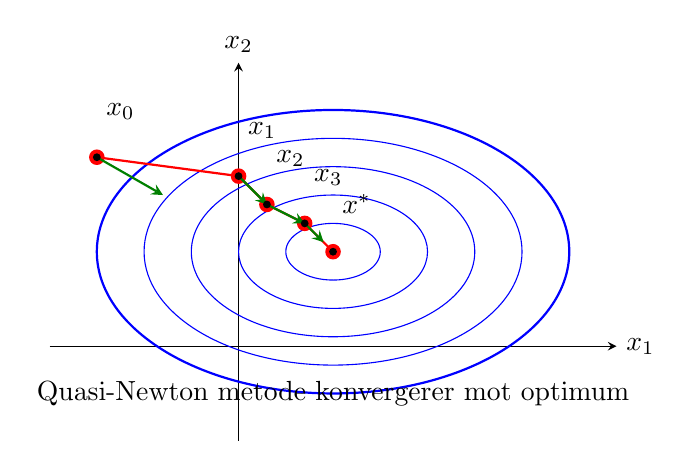
\begin{tikzpicture}[
			scale=1.2,
			>=stealth,
			point/.style={circle,fill=black,inner sep=1pt},
		]

		% Koordinatsystem
		\draw[->] (-2,0) -- (4,0) node[right]{$x_1$};
		\draw[->] (0,-1) -- (0,3) node[above]{$x_2$};

		% Elliptiske nivålinjer for en kvadratisk funksjon
		\draw[blue, thick] (1,1) ellipse (2.5 and 1.5);
		\draw[blue] (1,1) ellipse (2 and 1.2);
		\draw[blue] (1,1) ellipse (1.5 and 0.9);
		\draw[blue] (1,1) ellipse (1 and 0.6);
		\draw[blue] (1,1) ellipse (0.5 and 0.3);

		% Optimeringsbane
		\draw[mark=*, red, thick, mark size=2pt] plot coordinates {
				(-1.5, 2)
				(0, 1.8)
				(0.3, 1.5)
				(0.7, 1.3)
				(1, 1)
			};

		% Gradient piler
		\draw[->, green!50!black, thick] (-1.5, 2) -- (-0.8, 1.6);
		\draw[->, green!50!black, thick] (0, 1.8) -- (0.3, 1.5);
		\draw[->, green!50!black, thick] (0.3, 1.5) -- (0.7, 1.3);
		\draw[->, green!50!black, thick] (0.7, 1.3) -- (0.9, 1.1);

		% Legg til punkter for tydelighet
		\node[point, label={[shift={(0.3,0.3)}]$\symbf{x}_0$}] at (-1.5, 2) {};
		\node[point, label={[shift={(0.3,0.3)}]$\symbf{x}_1$}] at (0, 1.8) {};
		\node[point, label={[shift={(0.3,0.3)}]$\symbf{x}_2$}] at (0.3, 1.5) {};
		\node[point, label={[shift={(0.3,0.3)}]$\symbf{x}_3$}] at (0.7, 1.3) {};
		\node[point, label={[shift={(0.3,0.3)}]$\symbf{x}^\ast$}] at (1, 1) {};

		% Figurtittel
		\node at (1, -0.5) {Quasi-Newton metode konvergerer mot optimum};

	\end{tikzpicture}
	\caption{Illustrasjon av Quasi-Newton-iterasjoner som konvergerer mot løsningen langs en ikke-lineær vei. De elliptiske konturene representerer nivålinjer for objektfunksjonen, og punktene viser iterasjonene fra \(\symbf{x}_0\) til den optimale løsningen \(\symbf{x}^\ast\).}
	\label{fig:quasi_newton_convergence}
\end{figure}

\subsection{Limited Memory BFGS (L-BFGS)}
For høydimensjonale problemer kan det å lagre hele Hesse-approksimasjonen være vanskelig.
Limited Memory BFGS (L-BFGS) lagrer kun de siste \(m\) parene \((\symbf{s}_k, \symbf{y}_k)\) og konstruerer approksimasjonen implisitt.


\subsection{Egenskaper ved Quasi-Newton metoder}

\paragraph{Fordeler}
\begin{itemize}
	\item Raskere enn gradientbaserte metoder
	\item Lavere kostnad per iterasjon enn Newtons metode
	\item Bygger opp kurvaturinformasjon iterativt
	\item Superlineær konvergens under passende betingelser
\end{itemize}

\paragraph{Ulemper}
\begin{itemize}
	\item Langsommere konvergens enn ren Newton-metode lokalt
	\item Kan kreve flere linjesøk
	\item Sensitiv til nøyaktigheten i linjesøket, spesielt for DFP
\end{itemize}


For å sikre at Hesse-approksimasjonen forblir positiv definit, er det viktig at:

\begin{itemize}
	\item \(\symbf{y}_k^T\symbf{s}_k > 0\) (oppfylt under sterke Wolfe-betingelser)
	\item Initialmatrisen \(\symbf{B}_0\) eller \(\symbf{H}_0\) er positiv definit (ofte satt til \(\symbf{I}\))
\end{itemize}

En vanlig tilnærming for å forbedre ytelsen er å skalere den innledende approksimasjonen:

\[
	\symbf{H}_0 = \frac{\symbf{y}_k^T\symbf{s}_k}{\symbf{y}_k^T\symbf{y}_k}\symbf{I}
\]

Dette gir et bedre estimat for den faktiske skaleringen av den inverse Hesse-matrisen.

\subsection{Superlineær konvergens av Quasi-Newton metoder}

Under visse forutsetninger kan kvasi-Newton-metoder oppnå \textit{superlineær konvergens}. Dette skjer dersom søkeretningen \( \symbf{p}_k \) tilfredsstiller
\[
	\lim_{k \to \infty} \frac{\| (B_k - \nabla^2 f(\symbf{x}^\ast)) \symbf{p}_k \|}{\|\symbf{p}_k\|} = 0,
\]
hvor \( \symbf{x}_k \to \symbf{x}^\ast \) og \( \nabla^2 f(\symbf{x}^\ast) \succ 0 \). Dette innebærer at det ikke er nødvendig at \( B_k \to \nabla^2 f(\symbf{x}^\ast) \) i alle retninger – det er tilstrekkelig at tilnærmingen er god i retningen \( \symbf{p}_k \). Dette er en viktig og litt overraskende egenskap ved kvasi-Newton-metoder.

\begin{theorem}{Superlineær konvergens for kvasi-Newton}{quasi_newton_superlinear}
	La \( f : \mathbb{R}^n \to \mathbb{R} \) være to ganger kontinuerlig deriverbar. Anta at iterasjonene \( \symbf{x}_{k+1} = \symbf{x}_k + \alpha_k \symbf{p}_k \) bruker søkeretninger \( \symbf{p}_k \) som er desentrerte, og at steglengdene \( \alpha_k \) tilfredsstiller Wolfe-betingelsene med \( c_1 \le 1/2 \). Hvis \( \symbf{x}_k \to \symbf{x}^\ast \), hvor \( \nabla f(\symbf{x}^\ast) = 0 \) og \( \nabla^2 f(\symbf{x}^\ast) \) er positivt definit, og hvis
	\[
		\lim_{k \to \infty} \frac{\| \nabla f(\symbf{x}_k) + \nabla^2 f(\symbf{x}_k) \symbf{p}_k \|}{\|\symbf{p}_k\|} = 0,
	\]
	da gjelder:
	\begin{enumerate}
		\item Det finnes et \( k_0 \) slik at \( \alpha_k = 1 \) blir akseptert for alle \( k > k_0 \).
		\item Dersom \( \alpha_k = 1 \) for alle \( k > k_0 \), konvergerer \( \{\symbf{x}_k\} \) superlineært mot \( \symbf{x}^\ast \).
	\end{enumerate}
\end{theorem}

I kvasi-Newton-metoder er søkeretningen gitt ved \( \symbf{p}_k = -B_k^{-1} \nabla f_k \), og tilhørende tilstand for superlineær konvergens kan formuleres som:

\begin{theorem}{Nødvendig og tilstrekkelig betingelse for superlineær konvergens}{quasi_newton_superlinear_condition}
	Anta at \( f : \mathbb{R}^n \to \mathbb{R} \) er to ganger kontinuerlig deriverbar, og at \( \symbf{x}_k \to \symbf{x}^\ast \), der \( \nabla f(\symbf{x}^\ast) = 0 \) og \( \nabla^2 f(\symbf{x}^\ast) \) er positivt definit. Anta videre at iterasjonen er gitt ved
	\[
		\symbf{x}_{k+1} = \symbf{x}_k + \symbf{p}_k,
	\]
	hvor \( \symbf{p}_k = -B_k^{-1} \nabla f(\symbf{x}_k) \). Da konvergerer \( \{\symbf{x}_k\} \) superlineært mot \( \symbf{x}^\ast \) hvis og bare hvis
	\[
		\lim_{k \to \infty} \frac{\| (B_k - \nabla^2 f(\symbf{x}^\ast)) \symbf{p}_k \|}{\|\symbf{p}_k\|} = 0.
	\]
\end{theorem}

Dette viser at superlineær konvergens kan oppnås selv om \( B_k \not\to \nabla^2 f(\symbf{x}^\ast) \) i operatornorm - det er nok at \( B_k \) tilnærmer Hesse-matrisen godt langs retningene \( \symbf{p}_k \).

Under passende betingelser viser Quasi-Newtons metoder superlineær konvergens:

\[
	\lim_{k \to \infty} \frac{\|\symbf{x}_{k+1} - \symbf{x}^\ast\|}{\|\symbf{x}_k - \symbf{x}^\ast\|} = 0
\]
Selv om denne konvergensraten er langsommere enn Newtons kvadratiske konvergens, er kostnaden per iterasjon betydelig lavere, noe som gir en mer effektiv algoritme totalt sett, spesielt for store problemer.

\chapter{Optimal Steglengde \texorpdfstring{\(\alpha\)}{alpha}}
\label{chap:step_length_methods}
Steglengdemetoder er en viktig del av optimeringsalgoritmer, spesielt i gradientbaserte metoder som Newtons metode og Quasi-Newton-metoder.

De har som mål å bestemme den optimale steglengden \(\alpha\) for å minimere objektfunksjonen \(f\) langs en gitt retning \(p\).

Disse metodene er avgjørende for å sikre at algoritmen konvergerer mot en løsning på en effektiv måte.

\section{Linjesøk Metoder}
Linjesøk har som mål å finne en optimal steglengde \(\alpha_k\) i en gitt retning \(p_k\) for å minimere objektfunksjonen \(f\).

\begin{definition}{Linjesøk}{line_search}
	Gitt en nåværende iterasjon \(x_k\) og en søkeretning \(p_k\), finner linjesøk en steglengde \(\alpha_k > 0\) slik at
	\[
		x_{k+1} = x_k + \alpha_k p_k
	\]
	gir tilstrekkelig reduksjon i \(f\) langs retningen \(p_k\).
\end{definition}

For å oppnå dette, må vi oppfylle visse betingelser for \(\alpha_k\).
De varierer i hvor strenge krav de stiller til reduksjonen i funksjonsverdien, gradientens/Hesse-matrisens oppførsel og forholdet mellom disse.
De mest kjente er Wolfe-betingelsene, Armijo-betingelsen, Goldstein-betingelsen, kurvbetingelsen og Strong Wolfe-betingelsene.

\subsection{Wolfe-betingelsene}
Wolfe-betingelsene er en samling av betingelser som sikrer at linjesøket gir tilstrekkelig reduksjon i funksjonsverdien og at gradienten ikke endrer retning for brått.


\begin{align}
	f(x_k + \alpha_k p_k)              & \leq f(x_k) + c_1 \alpha_k \nabla f(x_k)^T p_k \tag{Armijo betingelse} \\
	\nabla f(x_k + \alpha_k p_k)^T p_k & \geq c_2 \nabla f(x_k)^T p_k \tag{Krumningsbetingelse}
\end{align}

der \(0 < c_1 < c_2 < 1\) er konstanter, typisk \(c_1 \approx 10^{-4}\) og \(c_2 \approx 0.9\).

\begin{definition}{Wolfe-betingelsene}{wolfe_conditions}
	\textbf{Armijo-betingelsen}:
	\begin{align*}
		f(\symbf{x} + \alpha \symbf{d})                    & \le f(\symbf{x}) + \beta\,\alpha\,\nabla f(\symbf{x})^T \symbf{d} \tag{Armijo} \\
		\nabla f(\symbf{x} + \alpha \symbf{d})^T \symbf{d} & \ge \rho \,\nabla f(\symbf{x})^T \symbf{d} \tag{Krumningsbetingelse}
	\end{align*}
\end{definition}

\begin{lemma}{Well-posedness av Wolfe-betingelsene}{well_posedness_wolfe_conditions}
	Anta at \(f:\R^n \to \R \) er kontinuerlig deriverbar. La \(\mathbf{p}_k\) være nedstigningsretningen ved iterasjon \(\mathbf{x}_k\), og anta at \(f\) er bundet nedenfra langs strålen:

	\[
		\{\mathbf{x}_k + \alpha \mathbf{p}_k : \alpha > 0\} \subset \mathbb{R}^n.
	\]

	\medskip

	Hvis \(0 < c_1 < c_2 < 1\), så eksisterer det intervaller av steglengder \(\alpha_k > 0\) slik at både Wolfe-betingelsene~\ref{def:wolfe_conditions} og Strong Wolfe-betingelsene~\ref{def:strong_wolfe_conditions} er oppfylt.

\end{lemma}

\subsection{Armijo-betingelsen}
\begin{definition}{Armijo-betingelsen}{armijo_condition}
	Armijo-betingelsen sikrer at steget gir en tilstrekkelig reduksjon i funksjonsverdien. Den krever at
	\[
		f(\symbf{x} + \alpha \symbf{d})
		\;\le\;
		f(\symbf{x})
		\;+\;
		\beta\,\alpha\,\nabla f(\symbf{x})^T \symbf{d},
	\]
	hvor \(\beta\) er en liten positiv konstant. Dette tilsier at \(f\) reduseres i tråd med en lineær modell.
\end{definition}

\begin{figure}[H]
	\centering
	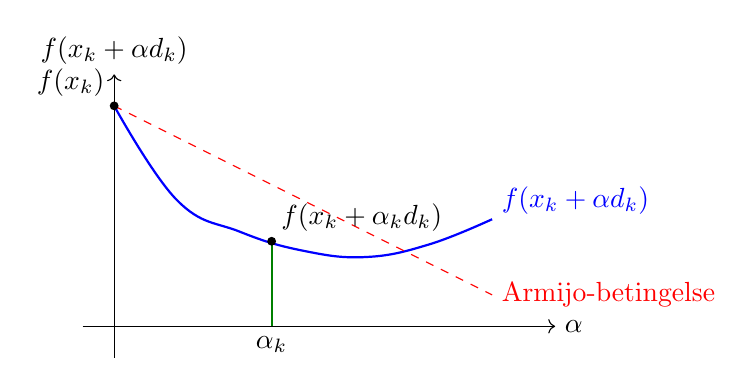
\begin{tikzpicture}[scale=0.8]
		% Axis
		\draw[->] (-0.5,0) -- (7,0) node[right]{$\alpha$};
		\draw[->] (0,-0.5) -- (0,4) node[above]{$f(\symbf{x}_k + \alpha \symbf{d}_k)$};

		% Function curve
		\draw[thick, blue] plot[smooth, tension=0.7] coordinates {(0,3.5) (1,2) (2,1.5) (3,1.2) (4,1.1) (5,1.3) (6,1.7)};

		% Armijo condition line
		\draw[red, dashed] plot coordinates {(0,3.5) (6,0.5)};

		% Initial point
		\fill (0,3.5) circle (2pt) node[above left]{$f(\symbf{x}_k)$};

		% Step point
		\draw[green!50!black, thick] (2.5,0) -- (2.5,1.35);
		\fill (2.5,1.35) circle (2pt) node[above right]{$f(\symbf{x}_k + \alpha_k \symbf{d}_k)$};

		% Step length label
		\node[below] at (2.5,0) {$\alpha_k$};

		% Legend
		\node[blue, right] at (6,2) {$f(\symbf{x}_k + \alpha \symbf{d}_k)$};
		\node[red, right] at (6,0.5) {Armijo-betingelse};
	\end{tikzpicture}
	\caption{Illustrasjon av linjesøk. Den blå kurven viser funksjonen langs søkeretningen, mens den røde stiplede linjen viser Armijo-betingelsen. Steglengden $\alpha_k$ gir tilstrekkelig reduksjon.}
\end{figure}

\subsection{Goldstein-betingelsen}
\begin{definition}{Goldstein-betingelsen}{goldstein_condition}
	Goldstein-betingelsen krever at den nye funksjonsverdien etter steget ligger innenfor et avgrenset intervall:
	\[
		f(\symbf{x}) + (1-\beta)\,\alpha\,\nabla f(\symbf{x})^T \symbf{d}
		\;\le\;
		f(\symbf{x} + \alpha \symbf{d})
		\;\le\;
		f(\symbf{x}) + \beta\,\alpha\,\nabla f(\symbf{x})^T \symbf{d}.
	\]
	Dette forhindrer at vi tar et for lite eller for stort steg.
\end{definition}

\subsection{Kurvbetingelsen}
\begin{definition}{Curvature condition}{curvature_condition}
	Kurvbetingelsen ser på gradientens endring \(\nabla f\) etter steget \(\alpha\) og krever at:
	\[
		\abs*{\nabla f(\symbf{x} + \alpha \symbf{d})^T \symbf{d}} \le -\sigma \nabla f(\symbf{x})^T \symbf{d},
	\]
	for en konstant \(\sigma \in (0,1)\). Dette sikrer at gradienten ikke endrer retning for brått, og at man unngår “overkorrigering”.
\end{definition}

\subsection{Sterk Wolfe-betingelsene}
\begin{definition}{Strong Wolfe-betingelsene}{strong_wolfe_conditions}
	Strong Wolfe-betingelsene kombinerer Armijo-betingelsen\ref{def:armijo_condition} med kurvbetingelsen\ref{def:curvature_condition} slik at:
	\begin{align*}
		f(\symbf{x} + \alpha \symbf{d})                    & \leq f(\symbf{x}) + c_1 \alpha \nabla f(\symbf{x})^T \symbf{d} \\
		\nabla f(\symbf{x} + \alpha \symbf{d})^T \symbf{d} & = c_2 \nabla f(\symbf{x})^T \symbf{d}
	\end{align*}

	der \(0 < c_1 < c_2 < 1\) er konstanter, typisk \(c_1 \approx 10^{-4}\) og \(c_2 \approx 0.9\).
	\medskip
	Disse betingelsene sikrer at steget gir tilstrekkelig reduksjon i funksjonsverdien og at gradienten ikke endrer retning for brått.
\end{definition}

\subsection{Goldstein-Wolfe-betingelsene}
\begin{definition}{Goldstein-Wolfe-betingelsene}{goldstein_wolfe_conditions}
	Goldstein-Wolfe-betingelsene krever at Armijo- og Goldstein-betingelsene begge er oppfylt:
	\begin{enumerate}
		\item Armijo-betingelsen:
		      \[
			      f(\symbf{x} + \alpha \symbf{d})
			      \;\le\;
			      f(\symbf{x})
			      \;+\;
			      \beta\,\alpha\,\nabla f(\symbf{x})^T \symbf{d}.
		      \]
		\item Goldstein-betingelsen:
		      \[
			      f(\symbf{x}) + (1-\beta)\,\alpha\,\nabla f(\symbf{x})^T \symbf{d}
			      \;\le\;
			      f(\symbf{x} + \alpha \symbf{d})
			      \;\le\;
			      f(\symbf{x}) + \beta\,\alpha\,\nabla f(\symbf{x})^T \symbf{d}.
		      \]
	\end{enumerate}
\end{definition}

\begin{figure}[H]
	\centering
	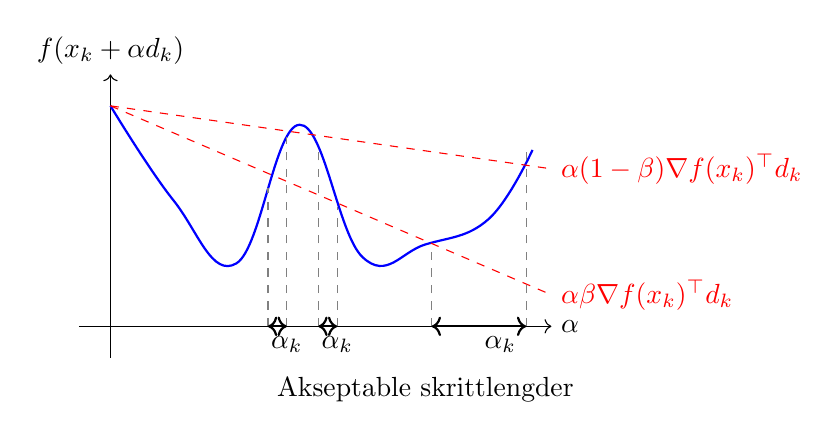
\begin{tikzpicture}[scale=0.8]
		% Akser
		\draw[->] (-0.5,0) -- (7,0) node[right]{$\alpha$};
		\draw[->] (0,-0.5) -- (0,4) node[above]{$f(\symbf{x}_k + \alpha \symbf{d}_k)$};

		% Funksjonskurve
		\draw[thick, blue] plot[smooth, tension=0.7] coordinates {(0,3.5) (1,2) (2,1) (3,3.2) (4,1.1) (5,1.3) (6,1.7) (6.7,2.8)};

		% Armijo øvre grense linje
		\draw[red, dashed] plot coordinates {(0,3.5) (7,0.5)} node[right]{$\alpha \beta \nabla f(\symbf{x}_k)^\top \symbf{d}_k$};
		% Goldstein øvre grense linje
		\draw[red, dashed] plot coordinates {(0,3.5) (7,2.5)} node[right]{$\alpha (1 - \beta) \nabla f(\symbf{x}_k)^\top \symbf{d}_k$};

		% Akseptable skrittlengder
		\draw[gray, dashed] (2.5,0) -- (2.5,2.2);
		\draw[gray, dashed] (2.8,0) -- (2.8,3.0);
		\draw[<->, thick] (2.5,0) -- (2.8,0) node[below]{$\alpha_k$};

		\draw[gray, dashed] (3.3,0) -- (3.3,2.8);
		\draw[gray, dashed] (3.6,0) -- (3.6,1.9);
		\draw[<->, thick] (3.3,0) -- (3.6,0) node[below]{$\alpha_k$};

		\draw[gray, dashed] (5.1,0) -- (5.1,1.2);
		\draw[gray, dashed] (6.6,0) -- (6.6,2.8);
		\draw[<->, thick] (5.1,0) -- (6.6,0) node[below left]{$\alpha_k$};

		% Legende
		\node at (5, -1) {Akseptable skrittlengder};



	\end{tikzpicture}
	\caption{Visualisering av Goldstein-Wolfe betingelsene.
		De akseptable skrittlengdene $\alpha$ ligger i området der funksjonen (blå kurve) er mellom Goldstein nedre grense og Armijo øvre grense (rød stiplet linje).}
	\label{fig:goldstein_wolfe_conditions}
\end{figure}

\subsection{Eksakt vs Ikke-Eksakt Linjesøk}

\begin{itemize}
	\item \textbf{Eksakt linjesøk}: Finn $\alpha_k$ som minimerer $f(x_k + \alpha p_k)$. Dette er ofte beregningsmessig dyrt.
	\item \textbf{Ikke-eksakt linjesøk}: Finn $\alpha_k$ som gir tilstrekkelig reduksjon, f.eks. ved å oppfylle Wolfe betingelsene.
\end{itemize}

Linjesøk omfatter metoder for å finne en egnet skrittlengde \(\alpha\) eller \(\alpha_k\) i en gitt retning \(\symbf{d}\) som reduserer objektfunksjonen \(f(\symbf{x})\).

\subsection{Backtracking Line Search}
Backtracking Line Search er en metode for å finne en passende skrittlengde \(\alpha\) som sikrer en ønsket reduksjon i \(f(\symbf{x})\) langs en retning \(\symbf{d}\).

\subsubsection{Algoritme}
\begin{algorithm}[H]
	\SetAlgoLined
	\KwIn{Startpunkt \( \symbf{x} \), retning \( \symbf{d} \), initial skrittlengde \( \alpha \), \textit{backtracking}-parameter \( \beta \in (0,1) \), \textit{skalering} \( \rho \in (0,1) \)}
	\KwOut{Skrittlengde \( \alpha \)}
	\While{\( f(\symbf{x} + \alpha \symbf{d}) > f(\symbf{x}) + \beta \,\alpha \,\nabla f(\symbf{x})^T \symbf{d} \)}{
		\(\alpha \leftarrow \rho \,\alpha\)
	}
	\caption{Backtracking Line Search (BLS)}
	\label{alg:backtracking_line_search}
\end{algorithm}

\subsection{Konvergens av Linjesøk}
\begin{theorem}{Konvergens av linjesøk}{line_search_convergence}
	Anta at \(f\) er kontinuerlig deriverbar og at det finnes en \(\alpha^\ast > 0\) slik at
	\[
		f(\symbf{x} + \alpha^\ast \symbf{d}) < f(\symbf{x}) + \beta\,\alpha^\ast\,\nabla f(\symbf{x})^T \symbf{d}.
	\]
	Da vil Backtracking Line Search konvergere til en skrittlengde \(\alpha_k\) som tilfredsstiller Armijo-betingelsen.
\end{theorem}

\begin{theorem}{Zoutendijk's result}{zoutendijk_result}
	La \( \symbf{x}_{k+1} = \symbf{x}_k + \alpha_k \symbf{p}_k \), hvor \( \mathbf{p}_k \) er en nedstigningsretning, med skrittlengde \( \alpha_k \) som tilfredsstiller Wolfe-betingelsene \ref{def:wolfe_conditions}.

	Anta at:
	\begin{itemize}
		\item \(f\) er bundet nedenfra i \(\R^n\)
		\item \(f\) er kontinuerlig deriverbar på det åpne settet \(\mathcal{N}\) som inneholder nivåsettet
		      \[ \mathcal{L} = \{\symbf{x}: f(\symbf{x}) \leq f(\symbf{x}_0)\} \]
		\item \(\nabla f\) er Lipschitz-kontinuerlig på \(\mathcal{N}\), dvs. det finnes en konstant \(L > 0\) slik at
		      \[ \|\nabla f(\symbf{x}) - \nabla f(\tilde{\symbf{x}})\| \leq L\|\symbf{x} - \tilde{\symbf{x}}\| \quad \text{for alle } \symbf{x}, \tilde{\symbf{x}} \in \mathcal{N} \]
	\end{itemize}

	Da har vi at:
	\[
		\sum_{k=0}^{\infty} \cos^2 \theta_k \| \nabla f(\symbf{x}_k) \|^2 < \infty,
	\]
	hvor \( \theta_k \) er vinkelen mellom \( \nabla f(\symbf{x}_k) \) og søkeretningen \( \symbf{p}_k \).

	Dette innebærer at \( \| \nabla f(\symbf{x}_k) \| \to 0 \) når \( k \to \infty \).

	\medskip

	Dette resultatet viser at hvis vi har en sekvens av iterasjoner \( \{ \symbf{x}_k \} \) som tilfredsstiller Wolfe-betingelsene, og hvis nivåsettet \( \mathcal{L} \) er begrenset og lukket (kompakt), så vil gradienten konvergere mot null.

\end{theorem}

\section{Trust Region}
\label{sec:trust_region}
Trust Region metoder er en klasse av optimeringsalgoritmer som skiller seg fra linjesøkmetoder ved at de bestemmer både retning og steglengde samtidig.
Det grunnleggende prinsippet er å definere et \emph{tillitsområde} rundt den nåværende iterasjonen \(\symbf{x}_k\), hvor vi antar at den kvadratiske modellen \(m_k(\symbf{p})\) gir en god tilnærming av objektfunksjonen \(f(\symbf{x})\).

I hver iterasjon løser metoden et begrenset optimeringsproblem av formen:
\[
	\min_{\symbf{p} \in \mathbb{R}^n} m_k(\symbf{p}) = f_k + \symbf{g}_k^T\symbf{p} + \frac{1}{2}\symbf{p}^T\symbf{B}_k\symbf{p} \quad \text{slik at} \quad \|\symbf{p}\| \leq \Delta_k
\]
hvor:
\begin{itemize}
	\item $f_k = f(\symbf{x}_k)$ er funksjonsverdien i nåværende punkt
	\item $\symbf{g}_k = \nabla f(\symbf{x}_k)$ er gradienten
	\item $\symbf{B}_k$ er en symmetrisk matrise som approksimerer Hesse-matrisen $\nabla^2 f(\symbf{x}_k)$
	\item $\Delta_k$ er radiusen til tillitsområdet
\end{itemize}

For optimeringsproblemer på formen \eqref{eq:unconstrained_optimization_problem} gir denne tilnærmingen flere fordeler:
\begin{itemize}
	\item Vi kan kontrollere kvaliteten på modellen ved å justere størrelsen på tillitsområdet
	\item Metoden kan håndtere ikke-konvekse problemer mer robust enn linjesøkmetoder
	\item Den kvadratiske modellen gir god lokal tilnærming når vi er nær et minimum
\end{itemize}


\begin{definition}{Trust Region}{trust_region}
	En \textbf{trust region} er et område rundt den nåværende iterasjonen \( \symbf{x}_k \) der vi antar at den kvadratiske modellen \( m_k(\symbf{p}) \) er en tilstrekkelig representasjon av objektfunksjonen \( f(\symbf{x}) \).
	\[
		\mathcal{D}_k = \{\symbf{x} : \|\symbf{x} - \symbf{x}_k\| \leq \Delta_k\}
	\]
	hvor \( \Delta_k \) er radiusen til trust regionen.
\end{definition}

\begin{figure}[H]
	\centering
	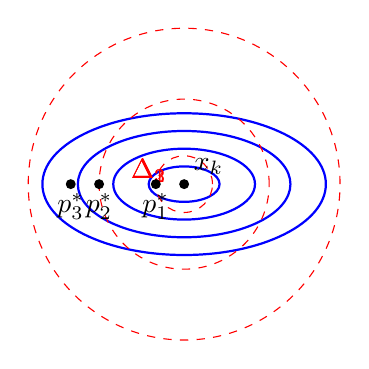
\begin{tikzpicture}[scale=0.9]
		% Konturlinjer for modellen
		\draw[blue, thick] (0,0) ellipse (2 and 1);
		\draw[blue, thick] (0,0) ellipse (1.5 and 0.75);
		\draw[blue, thick] (0,0) ellipse (1 and 0.5);
		\draw[blue, thick] (0,0) ellipse (0.5 and 0.25);

		% Forskjellige trust regions
		\draw[red, dashed] (0,0) circle (0.4) node[above left, xshift=-0.1cm, yshift=-0.1cm] {$\Delta_1$};
		\draw[red, dashed] (0,0) circle (1.2) node[above left, xshift=-0.1cm, yshift=-0.1cm] {$\Delta_2$};
		\draw[red, dashed] (0,0) circle (2.2) node[above left, xshift=-0.1cm, yshift=-0.1cm] {$\Delta_3$};

		% Nuværende punkt
		\fill (0,0) circle (2pt) node[above right] {$\symbf{x}_k$};

		% Løsningspunkter
		\fill (-0.4,0) circle (2pt) node[below] {$\symbf{p}_1^\ast$};
		\fill (-1.2,0) circle (2pt) node[below] {$\symbf{p}_2^\ast$};
		\fill (-1.6,0) circle (2pt) node[below] {$\symbf{p}_3^\ast$};

	\end{tikzpicture}
	\caption{Løsning av trust region-underproblemet for forskjellige radier $\Delta_1$, $\Delta_2$, $\Delta_3$. For liten radius ($\Delta_1$) ligger løsningen på grensen, for medium radius ($\Delta_2$) også på grensen, mens for stor radius ($\Delta_3$) er løsningen den ubegrensede minimanten.}
	\label{fig:trust_region_solutions}
\end{figure}

\subsection{Trust Region Algoritme}
Det viktigste i en trust region-algoritme er hvordan man velger trust region-radius $\Delta_k$ ved hver iterasjon. Dette valget baseres på forholdet $\rho_k$:
\[
	\rho_k = \frac{f(\symbf{x}_k) - f(\symbf{x}_k + \symbf{p}_k)}{m_k(\symbf{0}) - m_k(\symbf{p}_k)}
\]

\begin{algorithm}[H]
	\SetAlgoLined
	\KwIn{Startpunkt $\symbf{x}_0$, initial trust region radius $\Delta_0 > 0$, parametere $\hat{\Delta} > 0, \eta \in (0, \frac{1}{4})$ og $\gamma \in (0, \frac{1}{4})$}
	\KwOut{Løsning $\symbf{x}^\ast$}
	\For{$k = 0, 1, 2, \ldots$}{
		Finn steget $\symbf{p}_k$ med Cauchy- eller Dogleg-metoden.\\
		Beregn forholdet $\rho_k$.\\
		\uIf{$\rho_k < \frac{1}{4}$}{
			$\Delta_{k+1} \leftarrow \frac{1}{4}\Delta_k$
		}
		\Else{
			\uIf{$\rho_k > \frac{3}{4}$ \textbf{og} $\|\symbf{p}_k\| = \Delta_k$}{
				$\Delta_{k+1} \leftarrow \min(2\Delta_k, \hat{\Delta})$
			}
			\Else{
				$\Delta_{k+1} \leftarrow \Delta_k$
			}
		}
		\If{$\rho_k > \eta$}{
			$\symbf{x}_{k+1} \leftarrow \symbf{x}_k + \symbf{p}_k$
		}
		\Else{
			$\symbf{x}_{k+1} \leftarrow \symbf{x}_k$
		}
	}
	\caption{Trust Region Algoritme}
	\label{alg:trust_region}
\end{algorithm}

\begin{algorithm}[H]
	\SetAlgoLined
	\KwIn{Startpunkt \( x_0 \in \mathbb{R}^n \), initial radius \( \Delta_0 > 0 \), parametere \( 0 < \eta < 1 \), \( 0 < \gamma_1 < 1 < \gamma_2 \)}
	\KwOut{Løsning \( x^\ast \)}
	\For{\( k = 0, 1, 2, \dots \)}{
		Løs delproblemet for å finne et steg \( p_k \)\;
		Beregn forholdet:
		\[
			\rho_k = \frac{f(x_k) - f(x_k + p_k)}{m_k(0) - m_k(p_k)}
		\]\;
		Oppdater punktet:
		\[
			x_{k+1} = \begin{cases}
				x_k + p_k, & \rho_k \ge \eta, \\[6pt]
				x_k,       & \rho_k < \eta.
			\end{cases}
		\]\;
		Oppdater tillitsområdet:
		\[
			\Delta_{k+1} = \begin{cases}
				\gamma_2 \Delta_k, & \rho_k > \eta,       \\[6pt]
				\Delta_k,          & \rho_k \approx \eta, \\[6pt]
				\gamma_1 \Delta_k, & \rho_k < \eta.
			\end{cases}
		\]
	}
	\caption{Intuitivt øker vi tillitsområdet når modellen er god og krymper det når modellen er dårlig.}
	\label{alg:trust_region_2}
\end{algorithm}

\subsection{Tillitsområde-steg}
Stegene karakteriseres gjennom en første-ordens nødvendig optimalitetsbetingelse:
\begin{theorem}{Karakterisering av tillitsområde-steg}{trust_region_step}
	Punktet $\symbf{p}^\ast$ er løsning av trust-region delproblemet hvis og bare hvis
	\[
		(\symbf{B}_k + \lambda^\ast \symbf{I})\symbf{p}^\ast = -\nabla f(\symbf{x}_k), \quad \lambda^\ast (\Delta_k - \|\symbf{p}^\ast\|) = 0, \quad \symbf{B}_k + \lambda^\ast \symbf{I} \succeq 0, \quad \lambda^\ast \ge 0.
	\]
	Dette innebærer at enten ligger løsningen på grensen av området, eller den ligger innenfor med $\lambda^\ast = 0$.
\end{theorem}

\begin{proof}{}{}
	Hovedidéen i beviset av Teorem \ref{thm:trust_region_step} er å bruke Lagrange-multiplikatorer for å håndtere trust-region-betingelsen som en begrensning:

	\[
		\min_p m_k(p), \quad \text{s.t.} \quad \|p\|^2 - \Delta_k^2 \leq 0.
	\]

	Lagrangianen blir
	\[
		\mathcal{L}(p,\lambda) = m_k(p) + \lambda(\|p\|^2 - \Delta_k^2),
	\]
	og første-ordens betingelser leder til ligningssystemet i teoremet.
\end{proof}

\begin{theorem}{Karakterisering av Trust Region-løsningen}{trust_region_solution}
	En vektor $\symbf{p}^\ast$ er en global løsning av trust region-problemet
	\[
		\min_{\symbf{p} \in \mathbb{R}^n} m(\symbf{p}) = f + \symbf{g}^T\symbf{p} + \frac{1}{2}\symbf{p}^T\symbf{B}\symbf{p}, \quad \text{slik at} \quad \|\symbf{p}\| \leq \Delta,
	\]
	hvis og bare hvis $\symbf{p}^\ast$ er gyldig og det finnes en skalar $\lambda \geq 0$ slik at følgende betingelser er oppfylt:
	\begin{align}
		(\symbf{B} + \lambda\symbf{I})\symbf{p}^\ast & = -\symbf{g},                   \\
		\lambda(\Delta - \|\symbf{p}^\ast\|)         & = 0,                            \\
		(\symbf{B} + \lambda\symbf{I})               & \text{ er positiv semidefinit.}
	\end{align}
	hvor $\lambda \geq 0$ er en Lagrange-multiplikator.
\end{theorem}

Dette teoremet gir flere interessante tilfeller:
\begin{itemize}
	\item Når løsningen er strengt innenfor trust region ($\|\symbf{p}^\ast\| < \Delta$), har vi $\lambda = 0$ fra komplementaritetsbetingelsen, så $\symbf{B}\symbf{p}^\ast = -\symbf{g}$.
	\item Når løsningen ligger på grensen ($\|\symbf{p}^\ast\| = \Delta$), kan $\lambda > 0$, hvilket betyr at $\symbf{p}^\ast$ er kollineær med den negative gradienten av modellen.
\end{itemize}

Trust region-metoden justerer radiusen $\Delta_k$ basert på hvor godt modellen forutsier den faktiske funksjonsverdien. Dette gjøres ved å beregne forholdet:
\[
	\rho_k = \frac{f(\symbf{x}_k) - f(\symbf{x}_k + \symbf{p}_k)}{m_k(\symbf{0}) - m_k(\symbf{p}_k)}
\]

Hvis $\rho_k$ er nær 1, betyr det at modellen gir en god prediksjon, og vi kan utvide trust region-radiusen. Hvis $\rho_k$ er nær 0 eller negativ, reduserer vi radiusen siden modellen ikke er pålitelig over så store avstander.
For å karakterisere de eksakte løsningene av trust region-underproblemet, kan vi benytte følgende teorem som viser at løsningen $\symbf{p}^\ast$ tilfredsstiller:

\[
	(\symbf{B} + \lambda \symbf{I})\symbf{p}^\ast = -\symbf{g}
\]

For å bevise teoremet, har vi bruk for følgende lemma:

\begin{lemma}{Kvadratisk minimering}{quadratic_minimization}
	La \(m\) være den kvadratiske funksjonen definert ved
	\[
		m(\symbf{p}) = \symbf{g}^\top \symbf{p} + \frac{1}{2} \symbf{p}^\top \symbf{B}\symbf{p},
	\]
	hvor \(\symbf{B}\) er en symmetrisk matrise. Da gjelder følgende:
	\begin{enumerate}
		\item Hvis \(\symbf{B}\) er positiv semidefinit, er enhver \(\symbf{p}\) som tilfredsstiller \(\symbf{B}\symbf{p} = -\symbf{g}\) en global minimerer av \(m\).
		\item \(m\) oppnår et minimum hvis og bare hvis \(\symbf{B}\) er positiv semidefinit og \(\symbf{g}\) er i bildet til \(\symbf{B}\).
		\item \(m\) har en unik minimerer hvis og bare hvis \(\symbf{B}\) er positiv definit.
	\end{enumerate}
\end{lemma}

\begin{proof}{Bevis av Lemma \ref{lem:quadratic_minimization}}
	Vi beviser hver av de tre påstandene separat:

	\begin{enumerate}
		\item \textbf{Hvis \(\symbf{B}\) er positiv semidefinit, er enhver \(\symbf{p}\) som tilfredsstiller \(\symbf{B}\symbf{p} = -\symbf{g}\) en global minimerer av \(m\):}

		      Anta at \(\symbf{p}\) tilfredsstiller \(\symbf{B}\symbf{p} = -\symbf{g}\). For enhver \(\symbf{w} \in \mathbb{R}^n\) har vi:
		      \[
			      m(\symbf{p} + \symbf{w}) = m(\symbf{p}) + \symbf{w}^\top \symbf{B} \symbf{w}.
		      \]
		      Siden \(\symbf{B}\) er positiv semidefinit, følger det at \(\symbf{w}^\top \symbf{B} \symbf{w} \geq 0\). Dermed er \(m(\symbf{p} + \symbf{w}) \geq m(\symbf{p})\), og \(\symbf{p}\) er en global minimerer.

		\item \textbf{\(m\) oppnår et minimum hvis og bare hvis \(\symbf{B}\) er positiv semidefinit og \(\symbf{g}\) er i bildet til \(\symbf{B}\):}

		      \begin{itemize}
			      \item \textit{Hvis-delen:} Hvis \(\symbf{B}\) er positiv semidefinit og \(\symbf{g}\) er i bildet til \(\symbf{B}\), finnes det en \(\symbf{p}\) slik at \(\symbf{B}\symbf{p} = -\symbf{g}\). Fra punkt (1) følger det at \(m\) oppnår et minimum.
			      \item \textit{Bare hvis-delen:} Anta at \(m\) oppnår et minimum i \(\symbf{p}\). Da må \(\nabla m(\symbf{p}) = \symbf{B}\symbf{p} + \symbf{g} = 0\), som impliserer at \(\symbf{g}\) er i bildet til \(\symbf{B}\). Videre må \(\nabla^2 m(\symbf{p}) = \symbf{B}\) være positiv semidefinit for at \(\symbf{p}\) skal være et minimum.
		      \end{itemize}

		\item \textbf{\(m\) har en unik minimerer hvis og bare hvis \(\symbf{B}\) er positiv definit:}

		      \begin{itemize}
			      \item \textit{Hvis-delen:} Hvis \(\symbf{B}\) er positiv definit, er \(\symbf{B}\symbf{p} = -\symbf{g}\) et lineært system med en unik løsning. Dermed har \(m\) en unik minimerer.
			      \item \textit{Bare hvis-delen:} Anta at \(\symbf{B}\) ikke er positiv definit. Da finnes det en \(\symbf{w} \neq 0\) slik at \(\symbf{w}^\top \symbf{B} \symbf{w} = 0\). Dette impliserer at \(m(\symbf{p} + \symbf{w}) = m(\symbf{p})\), så minimereren er ikke unik, hvilket gir en motsigelse.
		      \end{itemize}
	\end{enumerate}
\end{proof}

\begin{proof}{Bevis av teorem \ref{thm:trust_region_solution}}{}
	Anta først at betingelsene er oppfylt med en \(\lambda \geq 0\). Fra Lemma \ref{lem:quadratic_minimization} følger det at \(\symbf{p}^\ast\) er et globalt minimum av \(m(\symbf{p}) + \frac{\lambda}{2} \|\symbf{p}\|^2\), og dermed også et globalt minimum av trust region-problemet.

	For motsatt retning, anta at \(\symbf{p}^\ast\) er en global løsning. Hvis \(\|\symbf{p}^\ast\| < \Delta\), er \(\symbf{p}^\ast\) en (ubundet) minimerer av \(m\), og \(\lambda = 0\) tilfredsstiller betingelsene.
	Hvis \(\|\symbf{p}^\ast\| = \Delta\), følger det fra KKT-betingelsene at det finnes en \(\lambda \geq 0\) slik at \((\symbf{B} + \lambda \symbf{I})\symbf{p}^\ast = -\symbf{g}\) og \((\symbf{B} + \lambda \symbf{I})\) er positiv semidefinit.
\end{proof}


\subsection{Cauchy-punkt}
Cauchy-punktet er det punktet langs retningen av den bratteste nedstigningen (steepest descent), som løser delproblemet enklest:

\[
	\symbf{p}_C = -\tau_k \frac{\Delta_k \nabla f(\symbf{x}_k)}{\norm*{\nabla f(\symbf{x}_k)}^2},
	\quad
	\tau_k = \frac{\norm*{\nabla f(\symbf{x}_k)}^2}{\nabla f(\symbf{x}_k)^\top \symbf{B}_k \nabla f(\symbf{x}_k)}.
\]


\subsection{Dogleg-metoden}
Dogleg--metoden kombinerer retningene fra Newton-steget og Cauchy-punktet i en brutt linje (\enquote{dogleg}).
\begin{itemize}
	\item Først langs Newton-retningen til Newton-punktet hvis det er innenfor trust-region.
	\item Ellers finner man skjæringspunktet med kanten av tillitsområdet.
\end{itemize}

\begin{figure}[H]
	\centering
	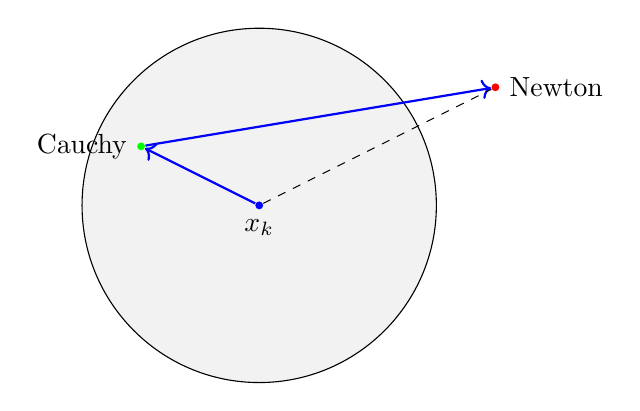
\begin{tikzpicture}[scale=1.5]
		\draw[fill=gray!10] (0,0) circle(1.5);
		\node[circle,fill=blue,inner sep=1pt,label=below:{$x_k$}] (xk) at (0,0) {};
		\node[circle,fill=red,inner sep=1pt,label=right:{Newton}] (N) at (2,1) {};
		\node[circle,fill=green,inner sep=1pt,label=left:{Cauchy}] (C) at (-1,0.5) {};
		\draw[thick,->,blue] (xk)--(C);
		\draw[thick,->,blue] (C)--(N);
		\draw[dashed] (xk)--(N);
	\end{tikzpicture}
	\caption{Dogleg-metoden kombinerer Cauchy-punktet og Newton-punktet.}
\end{figure}



\subsection{Trust Region vs Linjesøk}

\begin{itemize}
	\item \textbf{Trust region}: Først bestemmes hvor langt vi kan gå (radius \( \Omega_k \)), deretter bestemmes retningen og steglengden samtidig.
	\item \textbf{Linjesøk}: Først bestemmes retningen \( p_k \), deretter bestemmes hvor langt vi skal gå i den retningen (steplengde \( \alpha_k \)).
\end{itemize}

\chapter{Gradientfrie metoder}
\label{sec:gradientfrie_metoder}

Gradientfrie metoder er optimeringsalgoritmer som ikke benytter gradienter eller Hesse-matriser i søket etter et minimum.
De egner seg spesielt godt i situasjoner der objektfunksjonen \( f : \mathbb{R}^n \to \mathbb{R} \) er:
\begin{itemize}
	\item ikke-differensierbar eller stykkevis glatt,
	\item støyete, simulert eller svartboksbasert,
	\item kostbar eller upraktisk å derivere.
\end{itemize}

I stedet for å bruke analytisk eller numerisk informasjon om deriverte, evaluerer slike metoder funksjonsverdier i ulike retninger eller punktkombinasjoner, og gjør fremskritt basert på hvilke punkter som gir forbedring.

Gradientfrie metoder kan være svært effektive når informasjonen om objektfunksjonen er begrenset. De gir imidlertid sjelden noen garanti for å finne et globalt minimum, eller for konvergens i klassisk forstand.

\subsection{Heuristiske metoder}

En heuristisk metode er en algoritme som forsøker å finne en god (men ikke nødvendigvis optimal) løsning ved å bruke forenklede regler, prøve-og-feile-strategier eller strategier inspirert av natur og erfaring.

De er spesielt utviklet for problemer der klassiske metoder feiler - for eksempel når funksjonen har mange lokale minima, er ikke-glatt, støyete eller kun tilgjengelig gjennom simulering.

\paragraph{Egenskaper ved heuristiske metoder}

\begin{itemize}
	\item Utfører ofte globalt søk (f.eks. gjennom tilfeldige steg eller populasjoner).
	\item Krever ikke deriverte eller Hessian.
	\item Har lav til moderat regnekostnad.
	\item Mangler garanti for optimalitet, men gir ofte svært gode løsninger i praksis.
\end{itemize}

\subsection{Nelder--Mead-algoritmen}
\label{sec:nelder_mead}

Nelder--Mead er en populær algoritme  for å minimere funksjoner uten å bruke gradienter eller Hesse-matriser.
Den er særlig nyttig når funksjonen er \emph{ikke-glatt}, \emph{støyete} eller \emph{utilgjengelig i lukket form}.

Algoritmen bruker et \textbf{simplex}~\ref{def:simplex} (et geometrisk objekt med \( n+1 \) hjørner i \( n \)-dimensjonalt rom) i \( \mathbb{R}^n \) for å iterativt søke mot et lokalt minimum.

\begin{minipage}[t]{0.56\textwidth}
	Metoden manipulerer simplexen ved hjelp av \textbf{4 operasjoner}:
	\noindent
	\begin{itemize}
		\item \emph{Refleksjon}: Speiler det dårligste punktet gjennom tyngdepunktet
		\item \emph{Ekspansjon}: Strekker simplekset i lovende retninger
		\item \emph{Kontraksjon}: Krymper simplekset når refleksjon ikke gir forbedring
		\item \emph{Krymping}: Reduserer hele simplekset mot beste punkt
	\end{itemize}
	Gjennom disse operasjonene tilpasser simplekset seg automatisk til funksjonens form og \enquote{Kryper} mot det lokale minimum uten behov for deriverte.
\end{minipage}
\hfill
\begin{minipage}[t]{0.40\textwidth}
	\begin{figure}[H]
		\centering
		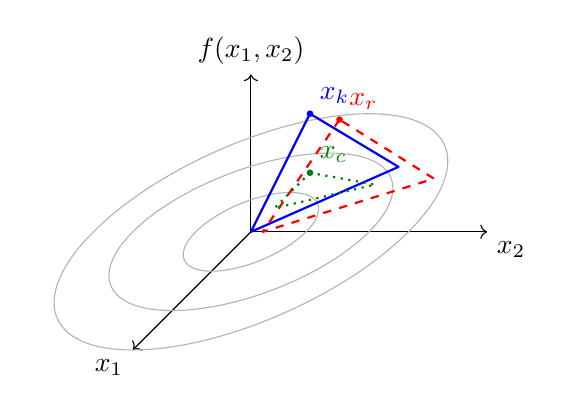
\begin{tikzpicture}[
				scale=1.0,
				x={(-0.5cm,-0.5cm)},
				y={(1cm,0cm)},
				z={(0cm,1cm)},
				line join=round
			]

			% Axes
			\draw[->] (0,0,0) -- (3,0,0) node[anchor=north east] {$x_1$};
			\draw[->] (0,0,0) -- (0,3,0) node[anchor=north west] {$x_2$};
			\draw[->] (0,0,0) -- (0,0,2) node[anchor=south] {$f(x_1,x_2)$};

			% Contours on base 
			\draw[black!30] (0,0,0) ellipse (3 and 2);
			\draw[black!30] (0,0,0) ellipse (2 and 1.5);
			\draw[black!30] (0,0,0) ellipse (1 and 0.7);

			% Initial simplex (blue solid) - scaled up by 1.5
			\draw[blue, thick]
			(1.5,1.5,2.25) -- (3,1.5,1.5) -- (2.25,3,1.95) -- cycle;

			% Reflected simplex (red dashed) - scaled up by 1.5
			\draw[red, thick, dashed]
			(0.75,1.5,1.8) -- (2.7,1.5,1.35) -- (1.65,3.15,1.5) -- cycle;

			% Contracted simplex (green dotted) - scaled up by 1.5
			\draw[green!50!black, thick, dotted]
			(1.8,1.65,1.65) -- (2.4,1.5,1.5) -- (1.95,2.55,1.575) -- cycle;

			% Key points only - scaled up by 1.5
			\fill[blue] (1.5,1.5,2.25) circle (1.2pt) node[above right] {$x_k$};
			\fill[red] (0.75,1.5,1.8) circle (1.2pt) node[above right] {$x_r$};
			\fill[green!50!black] (1.8,1.65,1.65) circle (1.2pt) node[above right] {$x_c$};

		\end{tikzpicture}
		\caption{Nelder-Mead algoritmen: Initialt (blå), reflektert (rød) og kontrahert (grønn) simplex med objektfunksjonens nivålinjer.}
		\label{fig:nelder_mead_3d}
	\end{figure}
\end{minipage}


\begin{algorithm}[H]
	\caption{Nelder--Mead-algoritme}
	\label{alg:nelder-mead}
	Initialiser simplex med \( n+1 \) punkter\;
	\Repeat{konvergenskriteriene er oppfylt}{
		Sorter simplex-punktene etter deres funksjonsverdi \( f(x_i) \)\;
		Beregn tyngdepunktet av de \( n \) beste punktene\;
		Reflekter det dårligste punktet gjennom tyngdepunktet for å få et nytt punkt \( x_r \)\;
		\uIf{\( f(x_1) \leq f(x_r) < f(x_n) \)}{
			Aksepter refleksjonen \( x_{n+1} \leftarrow x_r \)\;
		}
		\uElseIf{\( f(x_r) < f(x_1) \)}{
			Prøv ekspansjon til punkt \( x_e \)\;
			\If{\( f(x_e) < f(x_r) \)}{
				\( x_{n+1} \leftarrow x_e \)\;
			}
			\Else{
				\( x_{n+1} \leftarrow x_r \)\;
			}
		}
		\uElseIf{\( f(x_r) \geq f(x_n) \)}{
			Utfør en kontraksjon for å få punkt \( x_c \)\;
			\If{\( f(x_c) < f(x_{n+1}) \)}{
				\( x_{n+1} \leftarrow x_c \)\;
			}
			\Else{
				Krymp hele simplexet mot det beste punktet \( x_1 \)\;
			}
		}
	}
\end{algorithm}


\subsection{Andre gradientfrie metoder}

I tillegg til Nelder-Mead finnes det flere andre gradientfrie metoder:

\begin{itemize}
	\item \textbf{Genetiske algoritmer}: Inspirert av naturlig seleksjon, bruker populasjoner av løsninger som "evolusjonerer" over generasjoner.
	\item \textbf{Partikkelsverm-optimalisering (PSO)}: Inspirert av sosial atferd i fugleflokker eller fiskestimer, hvor partikler beveger seg i søkerommet.
	\item \textbf{Simulert annealing}: Inspirert av metallets varmebehandling, tillater algoritmen å akseptere dårligere løsninger med en viss sannsynlighet for å unngå å bli fanget i lokale minima.
\end{itemize}

\part{Betinget Optimering}

\chapter{Introduksjon til Betinget Optimering}

I dette kapittelet skal vi se på betinget optimering, som er en viktig del av optimeringsteori. Betinget optimering handler om å finne minimum eller maksimum av en funksjon når vi har begrensninger på variablene.

\section{Problemformulering}

Et typisk betinget optimeringsproblem kan skrives på formen:
\begin{align*}
	\min_{x \in \mathbb{R}^n} \quad & f(x)                                \\
	\text{betinget av} \quad        & g_i(x) \leq 0, \quad i = 1,\ldots,m \\
	                                & h_j(x) = 0, \quad j = 1,\ldots,p
\end{align*}

Her er:
\begin{itemize}
	\item $f(x)$ er målfunksjonen vi ønsker å minimere
	\item $g_i(x)$ er ulikhetsbetingelser
	\item $h_j(x)$ er likhetsbetingelser
\end{itemize}

Disse betingelsene definerer et tillatt område (feasible region) som løsningen må ligge innenfor.

\section{Grunnleggende definisjoner}

\begin{definition}{Lineært optimeringsproblem}{linear_programming}
	Et lineært optimeringsproblem er et optimeringsproblem på formen
	\begin{align*}
		\text{minimer}     & \quad \min_{x \in \R^n} f(x)                \\
		\text{betinget av} & \quad h_i(x) \leq 0, \quad i = 1, \ldots, m \\
		                   & \quad g_j(x) = 0, \quad j = 1, \ldots, p
	\end{align*}
	hvor \(f, h_i, g_j\) er lineære funksjoner.
\end{definition}

\begin{example}{Lineær funksjon}{linear_function}
	La \(f(\symbf{x}) = c^T\symbf{x} + d\) være en lineær funksjon, hvor \(c\) er en vektor normal til en hyperplan og \(d\) er en konstant.
	Da er \(f(\symbf{x}) = 0\) en lineær likning som definerer en hyperplan i \(\R^n\).
\end{example}

\begin{example}{Lineær regresjon}{linear_regression}
	La \(X \in \R^{n \times m}\) være en matrise med observasjoner og \(y \in \R^n\) være en vektor med målinger.
	Lineær regresjon er et eksempel på et lineært program hvor vi ønsker å finne en vektor \(w \in \R^m\) som minimerer kvadratfeilen
	\begin{equation*}
		\min_{w \in \R^m} \norm{Xw - y}_2^2.
	\end{equation*}
\end{example}

\section{Løsningsmetoder}

Vi skal se på ulike metoder for å løse betingede optimeringsproblemer, inkludert:
\begin{itemize}
	\item Lagranges multiplikatormetode for likhetsbetingelser
	\item KKT-betingelser for både likhets- og ulikhetsbetingelser
	\item Konveks optimering som en viktig spesialklasse
\end{itemize}

\chapter{Constraint Qualifications}

For å sikre at optimalitetsbetingelsene er gyldige og at vi kan finne Lagrange-multiplikatorer, trenger vi visse betingelser kjent som "constraint qualifications".

\section[Slaters betingelse]{\gls{slater-condition}}

\begin{definition}{Slater's Condition}{slater_condition}
	For a convex problem with inequality constraints
	\[
		c_i(x) \le 0,\quad i=1,2,\dots,m,
	\]
	Slater's condition holds if there exists an \(x\) such that
	\[
		c_i(x) < 0 \quad \text{for all } i.
	\]
\end{definition}

\begin{remark}{Intuition}{}
	This condition guarantees that the feasible region has a nonempty interior.

	In other words, the constraints are not all 'tight' at every point, which helps secure strong duality and the existence of Lagrange multipliers.
\end{remark}

\section{Lineær Uavhengighetsbetingelse (LICQ)}
\label{sec:LICQ}

I henhold til fremstillingen i \emph{Numerical Optimization} (2.~utgave) av Nocedal og Wright \cite[Kapittel~12]{NocedalWright}, betrakter vi et ikke-lineært optimeringsproblem av formen
\begin{equation}
	\label{eq:opt_problem}
	\begin{aligned}
		\min_{x \in \mathbb{R}^n}\quad & f(x)                                       \\
		\text{slik at}\quad
		                               & c_i(x) \;=\; 0, \quad i \in \mathcal{E},   \\[4pt]
		                               & c_j(x) \;\le\; 0, \quad j \in \mathcal{I}.
	\end{aligned}
\end{equation}
Her er \(f : \mathbb{R}^n \to \mathbb{R}\) en målfunksjon, og \(c_i(x)\), \(c_j(x)\) representerer henholdsvis likhets- og ulikhetsbetingelser.

\subsection{Definisjon av LICQ}

\begin{definition}{Linear Independence Constraint Qualification (LICQ)}{licq}
	La $x^*$ være et \emph{feasibelt} punkt. Definer mengden av aktive betingelser
	\[
		\mathcal{A}(x^*) \;=\; \{\; i \in \mathcal{E} \cup \mathcal{I} \;\mid\; c_i(x^*) = 0 \}.
	\]
	LICQ er oppfylt ved $x^*$ hvis gradientene til de aktive betingelsene
	\[
		\{\nabla c_i(x^*) :\, i \in \mathcal{A}(x^*)\}
	\]
	er lineært uavhengige i $\mathbb{R}^n$. Formelt betyr dette:
	\[
		\sum_{i \,\in\, \mathcal{A}(x^*)} \lambda_i \,\nabla c_i(x^*) \;=\; 0
		\quad \Longrightarrow \quad
		\lambda_i = 0 \;\;\text{for alle}\; i \in \mathcal{A}(x^*).
	\]
\end{definition}

\begin{remark}{Betydning av LICQ}{}
	LICQ sikrer at standard Karush--Kuhn--Tucker-(KKT)-teori er anvendelig, blant annet fordi:
	\begin{itemize}
		\item Eventuelle Lagrange-multiplikatorkoordinater (for de aktive betingelsene) er veldefinerte
		\item Disse multiplikatorene er ofte unike
		\item KKT-betingelsene blir nødvendige optimalitetsbetingelser
	\end{itemize}
\end{remark}

\subsection{Rollen til LICQ i KKT-teori}

Følgende punkter fremhever hvorfor LICQ er sentralt:
\begin{enumerate}
	\item \textbf{Eksistens av Lagrange-multiplierne:} Hvis \(x^*\) er et lokalt minimum og LICQ gjelder ved \(x^*\), eksisterer en unik vektor \(\lambda^*\) av multiplikatorer for de aktive betingelsene slik at KKT-betingelsene
	      \[
		      \nabla f(x^*) \;=\; \sum_{i \,\in\, \mathcal{A}(x^*)}\!\lambda_i^*\,\nabla c_i(x^*),\quad
		      \lambda_j^* \,\ge\,0 \text{ for aktive ulikheter},
	      \]
	      samt komplementaritetsbetingelser, blir oppfylt.
	\item \textbf{Lokal regularitet:} Dersom LICQ gjelder, har Jakobi-matrisen for de aktive betingelsene full rang. Dette er avgjørende for lokal analyse som benytter \emph{projisert Hessian} eller \emph{reduksjonsteknikker} i 2.~ordens formler.
	\item \textbf{Entydige multiplikatorer:} I mange realistiske problemer med LICQ vil multiplikatorene være unike for en gitt løsning \(x^*\), siden ingen lineær avhengighet i constraint-gradientene tillater alternative kombinasjoner.
\end{enumerate}
Skulle LICQ feile, kan mangfoldige eller manglende multiplikatorløsninger oppstå, eller KKT-metoder kan bryte sammen. Mer avslappede betingelser (f.eks.\ Mangasarian--Fromovitz) finnes, men garanterer ikke nødvendigvis entydighet av multiplikatorer.

\subsection{Geometrisk Intuisjon Gjennom Eksempler}

\paragraph{Eksempel~1: LICQ Gjelder.}

Anta at vi i \(\mathbb{R}^2\) har to betingelser:
\[
	\begin{aligned}
		c_1(x,y)\; & =\; x^2 + y^2 - 1\;=\;0, \\
		c_2(x,y)\; & =\; x - 0.5\;=\;0.
	\end{aligned}
\]
Den første representerer en sirkel (radius~1), og den andre en vertikal linje \(x=0.5\). Anta et felles punkt
\[
	P = \Bigl(0.5,\;\sqrt{3}/2\Bigr).
\]
Her er begge betingelsene aktive. Gradientene blir
\[
	\nabla c_1(P)\;=\;(2x,\,2y)\big\vert_{P}\;=\;(1,\,\sqrt{3}),
	\quad
	\nabla c_2(P)\;=\;(1,\,0).
\]
Siden disse ikke er skalar-multiple av hverandre, er de lineært uavhengige. Dermed er LICQ oppfylt ved \(P\).

\begin{tikzpicture}[scale=3]
	% Koordinatsystem
	\draw[->] (-1.2,0) -- (1.2,0) node[right] {$x$};
	\draw[->] (0,-1.2) -- (0,1.2) node[above] {$y$};

	% Sirkel: x^2 + y^2 = 1
	\draw (0,0) circle (1);

	% Linje x = 0.5
	\draw[red,thick] (0.5,-1) -- (0.5,1)
	node[above] {\(\,c_2: x=0.5\)};

	% Punkt P
	\coordinate (P) at (0.5,{sqrt(3)/2});
	\fill (P) circle (0.02) node[right]
		{\(\bigl(0.5,\tfrac{\sqrt{3}}{2}\bigr)\)};

	% Gradient c1 ved P (blå pil)
	\draw[->,blue,thick] (P) -- ++(0.3,0.5)
	node[above] {\(\nabla c_1\)};

	% Gradient c2 ved P (rød pil)
	\draw[->,red,thick] (P) -- ++(0.5,0)
	node[above right] {\(\nabla c_2\)};
\end{tikzpicture}

\paragraph{Eksempel~2: LICQ Feiler.}

Tenk deg følgende par av betingelser, igjen i \(\mathbb{R}^2\):
\[
	\begin{aligned}
		c_1(x,y)\; & =\;x^2 + y^2 - 1\;=\;0,      \\
		c_2(x,y)\; & =\;2\,(x^2 + y^2 - 1)\;=\;0.
	\end{aligned}
\]
Her er \(c_2\) bare en konstant multiplum av \(c_1\). Begge er aktive på samme sirkel \(x^2+y^2=1\). Gradientene er
\[
	\nabla c_1(x,y)=(2x,2y),\quad
	\nabla c_2(x,y)=2\,(2x,2y)=(4x,4y).
\]
De to gradientene er dermed kollineære for \emph{alle} punkter på sirkelen. Dette innebærer lineær avhengighet, så LICQ feiler.

\begin{center}
	\begin{tikzpicture}[scale=3]
		% Akser
		\draw[->] (-1.2,0) -- (1.2,0) node[right] {$x$};
		\draw[->] (0,-1.2) -- (0,1.2) node[above] {$y$};

		% Sirkel x^2 + y^2 = 1
		\draw (0,0) circle (1);

		% Et punkt Q på sirkelen
		\coordinate (Q) at (0.6,0.8);
		\fill (Q) circle (0.02) node[right]
			{\(\,(0.6,\,0.8)\)};

		% Gradient for c1 (blå pil)
		\draw[->,blue,thick] (Q) -- ++(0.3,0.4)
		node[above] {\(\nabla c_1\)};

		% Gradient for c2 (rød pil), kollineær
		\draw[->,red,thick] (Q) -- ++(0.6,0.8)
		node[above right] {\(\nabla c_2\)};
	\end{tikzpicture}
\end{center}
\paragraph{Eksempel~3: LICQ med flere ulikhetsbetingelser.}
La oss se på følgende optimeringsproblem:
\[
	\begin{aligned}
		\min_{x,y} \quad     & (x-1)^2 + (y+2)^2    \\
		\text{slik at} \quad & x \geq 0             \\
		                     & y \geq x-2           \\
		                     & (x-1)^2 + y^2 \geq 1
	\end{aligned}
\]

La oss definere følgende betingelser:
\[
	\begin{aligned}
		c_1(x,y) & = -x \leq 0            \\
		c_2(x,y) & = x-2-y \leq 0         \\
		c_3(x,y) & = 1-(x-1)^2-y^2 \leq 0
	\end{aligned}
\]

Med tilhørende gradienter:
\[
	\begin{aligned}
		\nabla c_1(x,y) & = (-1,0)        \\
		\nabla c_2(x,y) & = (1,-1)        \\
		\nabla c_3(x,y) & = (-2(x-1),-2y)
	\end{aligned}
\]

\begin{center}
	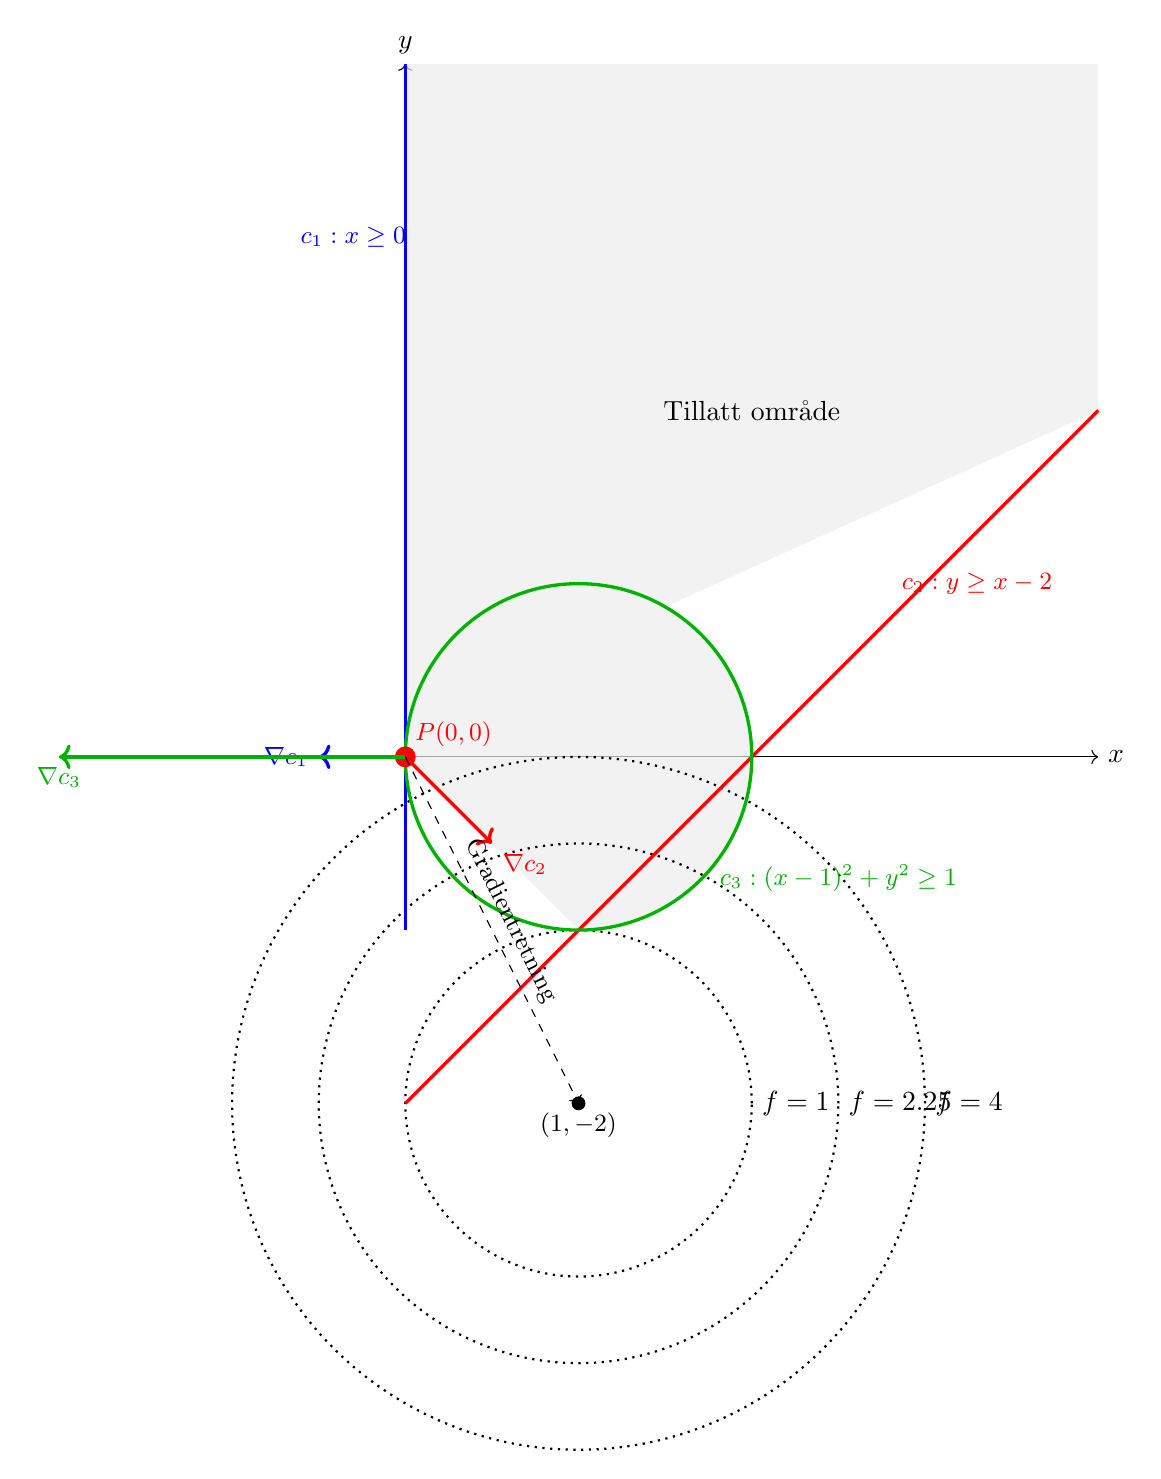
\begin{tikzpicture}[scale=2.2]
		% Koordinatsystem
		\draw[->] (-1,0) -- (4,0) node[right] {$x$};
		\draw[->] (0,-1) -- (0,4) node[above] {$y$};

		% Skravering av tillatt område først (under)
		\fill[gray!15, opacity=0.7] (0,0) -- (0,4) -- (4,4) -- (4,2) --
		plot[domain=60:0, smooth] ({1+cos(\x)},{sin(\x)}) --
		plot[domain=360:270, smooth] ({1+cos(\x)},{sin(\x)}) -- cycle;

		% Konturnivåer for målfunksjonen f(x,y) = (x-1)^2 + (y+2)^2
		\draw[black, dotted, thick] plot[domain=0:360,samples=100, smooth]
		({1+1.0*cos(\x)},{-2+1.0*sin(\x)}) node[right] {$f=1$};
		\draw[black, dotted, thick] plot[domain=0:360,samples=100, smooth]
		({1+1.5*cos(\x)},{-2+1.5*sin(\x)}) node[right] {$f=2.25$};
		\draw[black, dotted, thick] plot[domain=0:360,samples=100, smooth]
		({1+2.0*cos(\x)},{-2+2.0*sin(\x)}) node[right] {$f=4$};

		% Center point of objective function
		\fill[black] (1,-2) circle (0.04) node[below, font=\small] {$(1,-2)$};

		% x ≥ 0 (vertikal linje)
		\draw[blue, very thick] (0,-1) -- (0,4);

		% y ≥ x-2 (skrå linje)
		\draw[red, very thick] (0,-2) -- (4,2);

		% (x-1)^2 + y^2 ≥ 1 (sirkel med radius 1 sentrert i (1,0))
		\draw[green!70!black, very thick] (1,0) circle (1);

		% Forklarende tekst
		\node[blue, font=\small] at (-0.3,3) {$c_1: x \geq 0$};
		\node[red, font=\small] at (3.3,1) {$c_2: y \geq x-2$};
		\node[green!70!black, font=\small] at (2.5,-0.7) {$c_3: (x-1)^2 + y^2 \geq 1$};

		% Punkt der alle betingelser møtes (beregnet mer presist)
		\coordinate (P) at (0,0);
		\fill[red] (P) circle (0.06) node[above right, font=\small] {$P(0,0)$};

		% Gradienter ved punkt P
		\draw[->, very thick, blue] (P) -- +(-0.5,0) node[left, font=\small] {$\nabla c_1$};
		\draw[->, very thick, red] (P) -- +(0.5,-0.5) node[below right, font=\small] {$\nabla c_2$};
		\draw[->, very thick, green!70!black] (P) -- +(-2,0) node[below, font=\small] {$\nabla c_3$};

		% Feasible region label
		\node at (2,2) {Tillatt område};

		% Stiplet linje til optimal løsning
		\draw[black, dashed, ->] (P) -- (1,-2) node[midway, above, font=\small, sloped] {Gradientretning};
	\end{tikzpicture}
\end{center}

Ved punkt P hvor alle tre betingelser møtes, kan vi se at gradientene peker i forskjellige retninger og er lineært uavhengige. Derfor er LICQ oppfylt ved dette punktet. Dette er viktig for å kunne bruke KKT-betingelsene til å finne den optimale løsningen.
\subsection{Videre Merknader}

\begin{itemize}
	\item \textbf{Likhets- vs.\ ulikhetsbetingelser:} Likhetsbetingelsene \(c_i(x)=0\) er alltid aktive, mens en ulikhet \(c_j(x)\le 0\) kun er aktiv når \(c_j(x^*)=0\).
	\item \textbf{Jacobi-matrise:} Samler man gradientene som rader i en matrise, sier LICQ at denne matrisen har full rang, dvs. at antall aktive betingelser ikke overstiger \(\dim(x)\) og er lineært uavhengige.
	\item \textbf{Andre CQs:} Dersom LICQ ikke er oppfylt, kan man benytte andre såkalte \emph{constraint qualifications}, f.eks.\ Mangasarian--Fromovitz eller Slater-betingelser (for konvekse problemer), men da kan ikke entydigheten av multiplikatorer garanteres.
\end{itemize}

\subsection{Oppsummering}

Lineær Uavhengighetsbetingelse (LICQ) er en kjernenødvendighet for mange algoritmer og analytiske metoder innen ikke-lineær optimering. Den sikrer at de aktive betingelsene ved et punkt \(x^*\) er ``pent'' ordnet, i den forstand at ingen av gradientene er lineært avhengige. Når LICQ er gyldig, kan man utlede KKT-betingelsene og ofte fastslå entydige multiplikatorer. Som eksempel viser vi at betingelser som er multiple av hverandre (redundante) fører til brudd på LICQ og kan komplisere både teori og numeriske metoder.

\chapter{Optimalitetsbetingelser}

\section{Lagrangian-funksjonen}
\begin{definition}{The Lagrangian of a problem}{lagrangian}
	The Lagrangian of a problem is the function \(\mathcal{L}: \mathbb{R}^d \times \mathbb{R}^m \times \mathbb{R}^l \times \mathbb{R}^e \to \mathbb{R}\) defined as:
	\begin{align*}
		\mathcal{L}(x, \lambda, \mu, v) & = f(x) + \sum_{i\in \mathcal{I}} \lambda_i c_i(x) + \sum_{1 \leq i \leq m} \mu_i (Ax - b)_i + \sum_{1 \leq i \leq l} v_i (Cx - b)_i                               \\
		                                & = f(x) - \sum_{i \in \mathcal{I}} \lambda_i c_i(x) - \inner{\mu, Ax - b} - \inner{v, Cx - e}\footnote{\( (1) \iff \nabla_x \mathcal{L}(x, \lambda, \mu, v) = 0\)}
	\end{align*}
\end{definition}

Lagrangian-funksjonen gjør det mulig å håndtere betingelser ved å innføre multiplikatorer som vekter viktigheten av hver betingelse. Dette omformer et betinget optimeringsproblem til et ubetinget problem der vi søker sadelpunkter for Lagrangian-funksjonen.

\section{Farkas' lemma}

\begin{lemma}{Farka's Lemma}{farkas_lemma}
	Let \(A \in \mathbb{R}^{m \times n}\) and \(c \in \mathbb{R}^n\). Then, exactly one of the following statements is true:
	\begin{enumerate}
		\item[] \((1)\) There exists an \(x \in \mathbb{R}^n\) such that \(Ax \preceq 0\) and \(c^T x < 0\).
		\item[] \((2)\) There exists a \(y \in \mathbb{R}^m\) such that \(A^T y + c = 0\) and \(y \succeq 0\).
	\end{enumerate}
\end{lemma}

\begin{proof}
	\begin{enumerate}
		\item[] Assume that \((1)\) holds. Then \(Ax = b\) and \(x \ge 0\). If there exists a \(y\) such that \(y^T A \ge 0\), then
		      \[
			      y^T b = y^T Ax = (y^T A)x \ge 0,
		      \]
		      which contradicts \(y^T b < 0\).
		\item[] Assume that \((1)\) does not hold. We want to show that \((2)\) holds.

		      Let
		      \[
			      K = \{Ax \mid x \ge 0\}.
		      \]
		      Since \((1)\) does not hold, \(b \notin K\). Since \(K\) is a closed convex cone, by the separating hyperplane theorem, there exists a \(y \in \mathbb{R}^m\) such that
		      \[
			      y^T b < y^T z \quad \text{for all } z \in K.
		      \]
		      Since \(0 \in K\), we have \(y^T b < 0\).

		      Now, for any \(x \ge 0\), we have \(Ax \in K\), so \(y^T b < y^T Ax\).

		      Let \(x = e_i\), where \(e_i\) is the \(i\)-th standard basis vector. Then \(x \ge 0\), and
		      \[
			      y^T A e_i = (y^T A)_i > 0.
		      \]
		      Thus \(y^T A \ge 0\).
	\end{enumerate}

	\begin{center}
		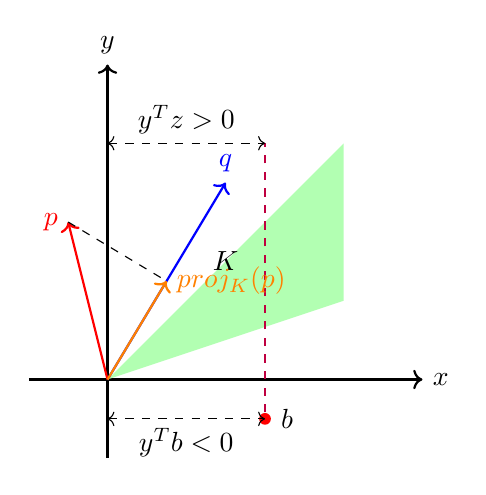
\begin{tikzpicture}
			\draw[->, thick] (-1, 0) -- (4, 0) node[right] {$x$};
			\draw[->, thick] (0, -1) -- (0, 4) node[above] {$y$};

			\fill[green!30] (0, 0) -- (3, 1) -- (3, 3) -- cycle;
			\node at (1.5, 1.5) {$K$};

			\node[circle, fill=red, inner sep=1.5pt, label=right:$b$] (b) at (2, -0.5) {};

			\draw[dashed, purple] (b) -- (2, 3);
			\draw[<->, dashed, black] (0, -0.5) -- (2, -0.5) node[midway, below, black] {$y^Tb < 0$};
			\draw[<->, dashed, black] (0, 3) -- (2, 3) node[midway, above, black] {$y^Tz > 0$};

			% Adding new vectors
			\draw[->, thick, blue] (0, 0) -- (1.5, 2.5) node[above] {$q$};
			\draw[->, thick, red] (0, 0) -- (-0.5, 2) node[left] {$p$};
			\draw[->, thick, orange] (0, 0) -- (0.75, 1.25) node[right] {$proj_K(p)$};
			\draw[dashed] (-0.5, 2) -- (0.75, 1.25);
		\end{tikzpicture}
	\end{center}

	The figure illustrates the geometric interpretation of Farkas' Lemma. The green region $K$ represents the cone of feasible points $\{Ax \mid x \ge 0\}$. The point $b$ (in red) lies outside this cone. The purple dashed line represents the separating hyperplane, which separates $b$ from $K$. Vector $p$ (in red) is projected onto the cone $K$, resulting in $proj_K(p)$ (in orange). Vector $q$ (in blue) lies inside the cone $K$. The black dashed lines show that the inner product $y^Tb$ is negative, while the inner product $y^Tz$ is positive for points $z$ in the cone $K$.
\end{proof}

\section[KKT-betingelser]{\gls{kkt-conditions}}

\begin{theorem}{KKT conditions}{kkt}
	\begin{align*}
		\mathcal{A}_1(x)            & := \{i \in \mathcal{I} \mid c_i(x) = 0\},                     \\
		\mathcal{A}_2(x)            & := \{1 \leq i \leq m \mid (Ax)_i = b_i\} \tag{Active indices} \\
		\text{Active indices at } x & \in \Omega                                                    \\
	\end{align*}

	\begin{itemize}
		\item \(A_i\) are the active constraints/indices at \(x\)
		\item \(C\) is the matrix of equality constraints.
		\item \(p\) is the direction of descent.
		\item \(x\) is the current point (feasible).
		\item \(T_{\Omega}(x)\) is the tangent cone at \(x\).
		\item \(c_i(x)\) is the value of the \(i\)-th constraint at \(x\).
		\item \(Ax\) is the value of the equality constraints at \(x\).
		\item \(b\) is the vector of equality constraints.
	\end{itemize}

	Assume that \emph{Slater's constraint} holds. Then, the following statements are equivalent:

	\begin{align*}
		p\in T_{\Omega}(x) & \Longleftrightarrow
		\begin{cases}
			\inner{\nabla c_i(x), p} \geq 0, & i \in \mathcal{A}_1(x) \\
			(Ax)_i \geq 0,                   & i \in \mathcal{A}_2(x) \\
			Cp = 0,                          &                        \\
		\end{cases}
	\end{align*}
\end{theorem}

\begin{theorem}{KKT conditions}{kkt_conditions}
	Assume \(c_i, i \in \mathcal{I}\) are concave in \(\mathcal{C}^1\),
	\(A\in \mathbb{R}^{m \times d}, b \in \mathbb{R}^m\) and \(C\in \mathbb{R}^{l \times d}\) and that \(f:\mathbb{R}^d \to \mathbb{R}\) is \(\mathcal{C}^1\). Assume that \emph{Slater's condition} holds.

	If \(x^\star\) is a local minimum of \(\min_x f(x)\) s.t.
	\[
		\begin{cases}
			c_i(x) \geq 0, & \forall i \in \mathcal{I} \\
			Ax \geq b,     &                           \\
			Cx = b,        &
		\end{cases}
	\]
	then there exists a \emph{Lagrange multipliers} \(\lambda^\star, \mu^\star\) with \(v \in \R^e\) s.t. the \emph{KKT conditions} hold:

	Then, the following statements are equivalent:
	\begin{align}
		\nabla f(x^\star) = \sum_{i\in \mathcal{I}} \lambda_i^\star \nabla c_i(x^\star) + A^T \mu^\star + C^T v^\star \\
		\begin{cases}
			c_i(x^\star) \geq 0, & \forall i \in \mathcal{I} \\
			Ax^\star \geq b,     &                           \\
			Cx^\star = e,        &                           \\
		\end{cases} \tag{Feasibility}                                                              \\
		\begin{cases}
			\lambda_i^\star \geq 0, & \forall i \in \mathcal{I} \\
			\mu_j^\star \in \geq 0, & \forall j \in \mathcal{J} \\
		\end{cases} \tag{Dual feasibility}                                                           \\
		\begin{cases}
			\lambda_i^\star c_i(x^\star) = 0, & \forall i \in \mathcal{I} \\
			\mu_j^\star C_j^T = 0,            & \forall j \in \mathcal{J} \\
		\end{cases} \tag{Complementary slackness}                                                 \\
		\begin{cases}
			\lambda_i^\star c_i(x^\star) = 0,      & \forall i \in \mathcal{I} \\
			\inner{\mu_j^\star, Ax^\star - b} = 0, & \forall j \in \mathcal{J} \\
		\end{cases} \tag{Complementary slackness}
	\end{align}
\end{theorem}

\begin{proof}{}{}
	We have the optimality condition:
	\[
		\inner{\nabla f(x^\star), p} \geq 0 \, \forall p \in T_{\Omega}(x^\star)
	\]
	\medskip
	\begin{align*}
		p \in T_{\Omega}(x^\star) \iff
		\begin{cases}
			\inner{\nabla c_i (x^\star), p }\geq 0                             & \forall i \in \mathcal{A}_1(x^\star) \\
			\text{or: there does not exist any } p \in \R^d \text{ such that:} &                                      \\
			\begin{cases}
				\inner{\nabla c_i (x^\star), p }\geq 0 & \forall i \in \mathcal{A}_1(x^\star) \\
				\inner{A_i^T , p }\geq 0               & \forall i \in \mathcal{A}_2(x^\star) \\
				\inner{ (C_i )^T, p } = 0              & \forall 1 \leq i \leq l              \\
				\inner{\nabla f (x^\star), p } < 0     &
			\end{cases}                             \\
			(Ap)_i \geq 0                                                      & \forall i \in \mathcal{A}_2(x^\star) \\
			Cp = 0                                                             &
		\end{cases}
	\end{align*}

	The second alternative is Farka's Lemma does not hold \(\implies\) The first holds.

	\begin{align*}
		\nabla f(x^\star) & = \sum_{i\in \mathcal{A}_1(x^\star)} \lambda_i^\star \nabla c_i(x^\star) + \sum_{i \in \mathcal{A}_2(x^\star)} \mu_i^\star A_i^T + \sum_{i=1}^l v_i^\star C_i^T \\
	\end{align*}

	For some  \(\lambda_i^\star \geq 0, \mu_i^\star \geq 0, v_i^\star \in \R\).

	Now define: \(\lambda_i^\star = 0 \) for \(i \notin \mathcal{A}_1(x^\star)\) and \(\mu_i^\star = 0\) for \(i \notin \mathcal{A}_2(x^\star)\).

	Then we have:
	\begin{align*}
		\nabla f(x^\star) & = \sum_{i\in \mathcal{I}} \lambda_i^\star \nabla c_i(x^\star) + \sum_{1 \leq i \leq m} \mu_i^\star A_i^T + \sum_{1 \leq i \leq l} v_i^\star C_i^T = \text{(1)} \\
	\end{align*}
	\qed
\end{proof}

\section{Geometrisk tolkning av KKT-betingelsene}

KKT-betingelsene har en klar geometrisk tolkning som er nyttig for å forstå deres betydning:

\begin{itemize}
	\item \textbf{Stasjonæritetsbetingelsen} (gradienten av Lagrangian er null) betyr at gradienten til målfunksjonen kan uttrykkes som en lineær kombinasjon av gradientene til de aktive betingelsene.
	\item \textbf{Primal feasibility} sikrer at løsningen tilfredsstiller alle opprinnelige betingelser.
	\item \textbf{Dual feasibility} (multiplikatorene for ulikheter er ikke-negative) sikrer at vi beveger oss i riktig retning langs betingelsene.
	\item \textbf{Komplementaritetsbetingelsen} forteller at en betingelse enten må være aktiv (likhet), eller så må den tilhørende multiplikatoren være null.
\end{itemize}

Denne geometriske tolkningen hjelper oss å visualisere hvordan KKT-betingelsene karakteriserer optimale punkter i et betinget optimeringsproblem.

\chapter{Konveks optimering}

\section{Egenskaper ved konvekse problemer}

Hvis et optimeringsproblem er konvekst, kan vi være sikre på at vi finner en global optimal løsning. Et konvekst optimeringsproblem har følgende egenskaper:
\begin{itemize}
	\item Målfunksjonen $f$ er konveks
	\item Likhetsbetingelsene $h_j$ er lineære (affine)
	\item Ulikhetsbetingelsene $g_i$ er konvekse
\end{itemize}

Konvekse optimeringsproblemer har flere fordelaktige egenskaper:
\begin{itemize}
	\item Ethvert lokalt minimum er også et globalt minimum
	\item KKT-betingelsene er både nødvendige og tilstrekkelige for optimalitet
	\item Det finnes effektive algoritmer for å løse konvekse problemer
\end{itemize}

\section{Dualitet i konveks optimering}

For konvekse optimeringsproblemer kan vi definere et dualt problem som gir en nedre grense på verdien av det primale problemet. Under visse betingelser, som Slaters betingelse, vil det primale og duale problemet ha samme optimale verdi - dette kalles "sterk dualitet".

Dualitetsteori gir oss viktige innsikter om optimale løsninger og multiplikatorer, og danner grunnlaget for mange effektive algoritmer for konveks optimering.

\clearpage

\appendix
\chapter{Formeltabell}

\begin{table}[H]
  \centering
  \footnotesize
  \begin{tabularx}{\textwidth}{@{}>{\color{black!70}}l>{\raggedright\arraybackslash}X@{}}
    \toprule
    \rowcolor{headerblue}
    \textbf{Term}     & \textbf{Definition/Formula}                                                                                                                               \\
    \midrule

    Convex            & \( f(\lambda x + (1-\lambda)y) \leq \lambda f(x) + (1-\lambda)f(y), \ \forall x,y \in \R^d, \lambda \in [0,1] \)                                          \\

    Coercive          & \( \lim_{\|x\| \to \infty} f(x) = \infty \) (ensures existence of minima)                                                                                 \\

    lsc               & \( \liminf_{x \to x_0} f(x) \geq f(x_0) \) (sublevel sets closed)                                                                                         \\

    Quasi-Convex      & \( \mathcal{L}_{f}(\alpha) = \{x \mid f(x) \leq \alpha\} \text{ convex } \forall \alpha \in \R \iff f(\lambda x + (1-\lambda)y) \leq \max\{f(x),f(y)\} \) \\

    Local Minimum     & \( \exists \epsilon > 0: f(x^*) \leq f(x), \, \forall x \in B_\epsilon(x^*) \)                                                                            \\

    Global Minimum    & \( f(x^*) \leq f(x), \, \forall x \in \R^d \)                                                                                                             \\

    Proximal Operator & \( \text{prox}_{\gamma f}(v) = \arg\min_x \left( f(x) + \frac{1}{2\gamma}\|x - v\|^2 \right) \)                                                           \\

    Subgradient       & \( g \in \partial f(x) \text{ if } f(y) \geq f(x) + g^\top(y-x), \, \forall y \in \R^d \)                                                                 \\

    Stochastic GD     & \( x_{k+1} = x_k - \eta_k \nabla f_{i_k}(x_k) \) (randomized gradients)                                                                                   \\

    Newton's Method   & \( x_{k+1} = x_k - [\nabla^2 f(x_k)]^{-1} \nabla f(x_k) \)                                                                                                \\
    \bottomrule
  \end{tabularx}
  \caption{Quick Reference: Key Definitions and Formulas}
\end{table}


\chapter{Funksjonsegenskaper og Optimeringsmetoder}
\begin{table}[ht]
  \centering
  \caption{Function Properties and Optimization Methods}
  \footnotesize
  \begin{tabularx}{\textwidth}{@{} >{\RaggedRight}Z Y Y Y Y Y Y Y @{}}
    \toprule
    \textbf{Function (Domain)}                                                        & \textbf{Cvx} & \textbf{Coe} & \textbf{lsc} & \textbf{QCvx} & \textbf{Loc} & \textbf{Glo} & \textbf{Alg}         \\
    \midrule

    \multicolumn{8}{@{}l}{\textbf{Scalar Functions (\(\R\))}}                                                                                                                                           \\
    \midrule
    \( f(x) = x^2 \)                                                                  & \yes         & \yes         & \yes         & \yes          & \yes         & \yes         & Gradient Descent     \\
    \( f(x) = |x| \)                                                                  & \yes         & \yes         & \yes         & \yes          & \yes         & \yes         & Proximal/Subgradient \\
    \( f(x) = x^3 \)                                                                  & \no          & \no          & \yes         & \no           & \no          & \no          & Heuristics           \\
    \( f(x) = x^4 - Cx^2 \)                                                           & \no          & \yes         & \yes         & \no           & \yes         & \yes         & Newton               \\
    \( f(x) = \begin{cases} 0 & x \leq 0 \\ 1 & x > 0 \end{cases} \)                  & \no          & \no          & \yes         & \yes          & \yes         & \yes         & Subgradient          \\

    \( f(x) = \sqrt{x}\ (x \geq 0) \)                                                 & \no          & \no          & \yes         & \yes          & \yes         & \yes         & Gradient Descent     \\
    \( f(x) = \log(1 + e^x) \)                                                        & \yes         & \yes         & \yes         & \yes          & \yes         & \yes         & Gradient Descent     \\
    \( f(x) = Ce^x \)                                                                 & \yes         & \no          & \yes         & \yes          & \no          & \no          & Heuristics           \\
    \( f(x) = e^x - x \)                                                              & \yes         & \yes         & \yes         & \yes          & \yes         & \yes         & Newton               \\
    \( f(x) = \sin(x) \)                                                              & \no          & \no          & \yes         & \no           & \yes         & \yes         & Heuristics           \\

    \midrule

    \multicolumn{8}{@{}l}{\textbf{Vector Functions (\(\R^d\))}}                                                                                                                                         \\
    \midrule
    \( f(\mathbf{x}) = \|\mathbf{x}\| \)                                              & \yes         & \yes         & \yes         & \yes          & \yes         & \yes         & Proximal             \\
    \( f(\mathbf{x}) = \|\mathbf{x}\| + \sin(x_1) \)                                  & \no          & \yes         & \yes         & \no           & \yes         & \yes         & Stochastic GD        \\
    \( f(\mathbf{x}) = \mathbf{x}^\top \mathbf{A} \mathbf{x}\ (\mathbf{A} \succ 0) \) & \yes         & \yes         & \yes         & \yes          & \yes         & \yes         & Newton               \\
    \midrule

    \multicolumn{8}{@{}l}{\textbf{Counterexamples}}                                                                                                                                                     \\
    \midrule
    \( f(x) = \sqrt{|x|} \)                                                           & \no          & \no          & \yes         & \yes          & \yes         & \yes          & Heuristics           \\
    \( f(x,y) = x^4y^2 + x^4 - 2x^3y \)                                               & \no          & \yes         & \yes         & \no           & \yes         & \yes         & Evolutionary         \\
    \bottomrule
  \end{tabularx}
  \label{tab:function_properties}
  \vspace{0.5em}
  \footnotesize
  \textbf{Key Corrections:}
  \begin{itemize}
    \item \( f(x) = |x| \): Marked as convex/coercive; algorithm changed to Proximal/Subgradient.
    \item \( f(x) = x^3 \): Corrected coerciveness (No) and minima (No).
    \item \( f(x) = \sqrt{x} \): Added domain restriction \( x \geq 0 \); has global minimum at 0.
    \item \( f(x) = \sin(x) \): Quasi-convexity corrected to No; has infinite global minima.
    \item Quadratic forms: Explicitly stated \( \mathbf{A} \succ 0 \) for convexity.
  \end{itemize}
\end{table}


\chapter{Lectures}
\clearpage

\section{Lecture 1 (6. Januar 2025)}

\subsection*{Eksistens av globale løsninger}

\begin{definition}{Nivåmengde}{level-set}
  For en funksjon  \(f: \R^d \to \R\) definerer vi nivåmengden som
  \[
    L_f(\alpha) = \{x \in \R^d : f(x) \leq \alpha\}
  \]
\end{definition}

\begin{theorem}{Karakterisering av koersivitet og semi-kontinuitet}{characterization}
  La  \(f: \R^d \to \R\) være en funksjon. Da har vi:
  \begin{itemize}
    \item  \(f\) er koersiv  \(\iff L_f(\alpha)\) er avgrenset for alle  \(\alpha < \infty\)
    \item  \(f\) er nedre semi-kontinuerlig (lsc)  \(\iff L_f(\alpha)\) er lukket for alle  \(\alpha\)
  \end{itemize}
\end{theorem}

\begin{theorem}{Eksistens av globale løsninger}{existence}
  Hvis  \(f: \R^d \to \R\) er koersiv og nedre semi-kontinuerlig, så har problemet
  \[
    \min_{x \in \R^d} f(x)
  \]
  en global løsning.
\end{theorem}

\subsection*{Nødvenige og tilstrekkelige betingelser for lokale løsninger}

\begin{theorem}{Nødvendige betingelser for lokale løsninger}{necessary-conditions}
  La  \(x^* \in \R^d\) være en lokal løsning av  \(\min_{x \in \R^d} f(x)\). Da gjelder:
  \begin{itemize}
    \item  \(\nabla f(x^*) = 0\) (Førsteordens nødvendig betingelse).
    \item  \(H_f(x^*)\) er positiv semi-definit (Andreordens nødvendig betingelse).
  \end{itemize}
  da er \(x^*\) en lokal løsning av  \(\min_{x \in \R^d} f(x)\).
\end{theorem}

\begin{theorem}{Tilstrekkelige betingelser for lokale løsninger}{sufficient-conditions}
  Hvis  \(x^* \in \R^d\) oppfyller:
  \begin{itemize}
    \item  \(\nabla f(x^*) = 0\) (Førsteordens betingelse)
    \item  \(H_f(x^*)\) er positiv definit (Andreordens tilstrekkelig betingelse)
  \end{itemize}
  da er  \(x^*\) en streng og isolert lokal løsning av  \(\min_{x \in \R^d} f(x)\).
\end{theorem}

\begin{example}{Eksistens og optimalitet}{}
  \begin{itemize}
    \item For \( f(x) = x^2 + 2x \), som er kontinuerlig og koersiv, finnes et globalt minimum i \( x^* = -1 \) der \( f(-1) = -1 \).
    \item For \( f(x) = x^2 \), har vi \( \nabla f(x) = 2x \). I \( x^* = 0 \) er \( \nabla f(0) = 0 \) og \( \nabla^2 f(x) = 2 > 0 \), som oppfyller SOSC.
  \end{itemize}
\end{example}

\section{Lecture 2 (10. January 2025)}

\subsection*{Gradientmetoder og konveksitet}

\begin{theorem}{Gradientestimat nær lokale minima}{gradient-estimate}
  La  \(f: \R^n \to \R\) være deriverbar og  \(x^*\) være et lokalt minimum. Da gjelder:
  \[
    \|\nabla f(x)\| \to 0 \quad \text{når } x \to x^*.
  \]
\end{theorem}

\begin{remark}{Geometrisk tolkning}
  Dette indikerer at funksjonen blir "flatere" når  \(x\) nærmer seg minimumpunktet, noe som er fundamentalt for konvergensen til iterative optimaliseringsmetoder.
\end{remark}

\begin{definition}{Konveks funksjon}{convex-function}
  En funksjon  \(f: \R^n \to \R\) er konveks hvis, for alle  \(x, y \in \R^n\) og  \(\lambda \in (0,1)\):
  \begin{align*}
    f(\lambda x + (1 - \lambda)y) \leq \lambda f(x) + (1 - \lambda)f(y) \tag{Konveks} \\
    f(\lambda x + (1 - \lambda)y) < \lambda f(x) + (1 - \lambda)f(y) \tag{Strengt konveks}
  \end{align*}
\end{definition}

\begin{remark}{Konveksitet med indre-produkt notasjon}{}
  En funksjon  \(f: \R^n \to \R\) er konveks hvis og bare hvis:
  \[
    f(y) \geq f(x) + \langle \nabla f(x), y - x \rangle
  \]
  for alle  \(x, y \in \R^n\).
\end{remark}

\begin{theorem}{Karakterisering av deriverbare konvekse funksjoner}{convex-characterization}
  For en deriverbar funksjon  \(f: \R^n \to \R\) er følgende ekvivalente:
  \begin{itemize}
    \item  \(f\) er konveks
    \item For alle  \(x, y \in \R^n\) gjelder:
          \[
            f(y) \geq f(x) + \nabla f(x)^\top (y - x)
          \]
  \end{itemize}
\end{theorem}

\begin{theorem}{Karakterisering av konvekse funksjoner med Hessian}{convex-hessian}
  For en dobbelt deriverbar funksjon  \(f: \R^n \to \R\) er følgende ekvivalente:
  \[
    f \text{ er konveks} \iff H_f(x) \succeq 0 \quad \forall x \in \R^n
  \]

  \(H_f(x) \succeq 0\) betyr at Hessian-matrisen er positiv semi-definit for alle  \(x\).

\end{theorem}

\begin{remark}{Positiv semi-definit matrise}
  En matrise  \(A \in \R^{n \times n}\) er positiv semi-definit hvis og bare hvis en av følgende ekvivalente påstander holder:
  \begin{align*}
    A \succeq 0 & \iff x^\top A x \geq 0 \quad \forall x \in \R^n \tag{Kvadratisk form}                         \\
                & \iff \lambda_i \geq 0 \text{ for alle egenverdier } \lambda_i \text{ av } A \tag{Egenverdier} \\
                & \iff \text{Alle hovedminordeterminanter er ikke-negative} \tag{Minordeterminanter}            \\
                & \iff A = LL^\top \text{ for en nedre triangulær matrise } L \tag{Cholesky}                    \\
                & \iff A = B^\top B \text{ for en matrise } B \in \R^{m \times n} \tag{Gram}                    \\
                & \iff A - 0 \cdot I \succeq 0 \tag{Semidefinit ordning}                                        \\
                & \iff A \text{ ligger i den positive semidefinite konen i } \R^{n \times n} \tag{PSD kone}     \\
                & \iff e^{tA} \text{ er positiv semidefinit for alle } t > 0 \tag{Matrise eksponential}
  \end{align*}

  \begin{itemize}
    \item Kvadratisk form:  \(x^\top A x \geq 0\) for alle  \(x \in \R^n\) karakteriserer positiv semi-definite matriser.
    \item Egenverdier: Alle egenverdier  \(\lambda_i\) av  \(A\) er ikke-negative.
    \item Hovedminordeterminant: Determinanten til alle hoved-undermatriser er ikke-negative.
          \[
            \begin{bmatrix}
              a_{11} & a_{12} \\
              a_{21} & a_{22}
            \end{bmatrix} \succeq 0 \iff a_{11} \geq 0, \quad a_{11}a_{22} - a_{12}a_{21} \geq 0
          \]

    \item Cholesky-faktorisering:  \(A = LL^\top\) der  \(L\) er en nedre triangulær matrise.
    \item Gram-matrise:  \(A = B^\top B\) der  \(B \in \R^{m \times n}\).
    \item Semidefinit ordning:  \(A - 0 \cdot I \succeq 0\) betyr at  \(A\) er positiv semi-definit.
    \item PSD-kone: Den positive semidefinite konen er mengden av alle positiv semi-definite matriser.
    \item Matrise eksponential:  \(e^{tA}\) er positiv semi-definit for alle  \(t > 0\).
  \end{itemize}
\end{remark}


\begin{theorem}{Globale egenskaper for konvekse funksjoner}{global-properties}
  La  \(f: \R^n \to \R\) være konveks. Da gjelder:
  \begin{itemize}
    \item Ethvert lokalt minimum er også et globalt minimum.
    \item Hvis  \(\nabla f(x^*) = 0\), da er  \(x^*\) et globalt minimum.
  \end{itemize}
\end{theorem}

\begin{example}{Konvekse funksjoner}{convex-examples}
  Noen klassiske eksempler på konvekse funksjoner:
  \begin{itemize}
    \item Lineære funksjoner:  \(f(x) = a^\top x + b\)
    \item Kvadratiske funksjoner med positiv definit matrise:  \(f(x) = x^\top Ax + b^\top x + c\), der  \(A \succ 0\)
    \item Eksponentialfunksjonen:  \(f(x) = e^{ax}\) for enhver  \(a \in \R\)
  \end{itemize}
\end{example}

\section{Lecture 3 (13. January 2025)}
\subsection*{Optimization Algorithms}

\begin{definition}{Nelder-Mead Algorithm}{nelder_mead}
  The Nelder-Mead algorithm is a heuristic search method used for minimizing an objective function without the need for derivatives. It operates on a simplex of \( n+1 \) points in \( \R^n \) and iteratively reflects, expands, contracts, or shrinks the simplex to converge to a local minimum.
\end{definition}

\begin{algorithm}[H]
  \caption{Nelder-Mead Algorithm}
  Initialize simplex with  \(n+1\) points\;
  \Repeat{convergence criteria are met}{
    Order the simplex points by their objective function values\;
    Compute the centroid of the best  \(n\) points\;
    Reflect the worst point through the centroid\;
    \uIf{reflected point is better than the second worst but not better than the best}{
      Accept the reflection\;
    }
    \uElseIf{reflected point is the best point}{
      Try expanding\;
    }
    \uElseIf{reflected point is worse than the second worst}{
      Perform contraction\;
    }
    \Else{
      Shrink the simplex towards the best point\;
    }
  }
\end{algorithm}

\subsubsection*{line search methods}
Line search methods aim to find an appropriate step size \( \alpha \) that sufficiently decreases the objective function along a given search direction \( d \). The goal is to ensure convergence and improve the efficiency of optimization algorithms.

\subsubsection*{Gradient Descent and Newton Directions}

\begin{definition}{Gradient Descent}{gradient-descent}
  Gradient descent is an iterative optimization algorithm that updates the current point \( x_k \) by moving in the opposite direction of the gradient:
  \[
    x_{k+1} = x_k - \alpha_k \nabla f(x_k)
  \]
  where \( \alpha_k \) is the step size.
\end{definition}

\begin{definition}{Newton Direction}{newton-direction}
  Newton's method uses second-order information by incorporating the Hessian matrix:
  \[
    x_{k+1} = x_k - [\nabla^2 f(x_k)]^{-1} \nabla f(x_k)
  \]
  This direction can provide faster convergence near the optimum.
\end{definition}

\subsubsection*{Armijo Condition for Step-Length Selection}

\begin{definition}{Armijo Condition}{armijo}
  The Armijo condition ensures that the step size \( \alpha \) provides a sufficient decrease in the objective function:
  \[
    f(x_k + \alpha d_k) \leq f(x_k) + c \alpha \nabla f(x_k)^\top d_k
  \]
  where \( 0 < c < 1 \) is a constant.
\end{definition}

\subsubsection*{Backtracking Line Search}

\begin{definition}{Backtracking Line Search}{backtracking}
  Backtracking line search starts with an initial step size and iteratively reduces it by a factor until the Armijo condition is satisfied.

\end{definition}

\begin{algorithm}[H]
  \caption{Backtracking Line Search}
  \label{alg:backtracking}
  \SetKwFunction{BacktrackingLineSearch}{BacktrackingLineSearch}
  \BacktrackingLineSearch{ \(x_k\),  \(d_k\),  \(f\),  \(\nabla f\),  \(\alpha\),  \(\rho\),  \(c\)}\;
  \While{ \(f(x_k + \alpha d_k) > f(x_k) + c \alpha \nabla f(x_k)^\top d_k\)}{
    \(\alpha \gets \rho \alpha\)\;
  }
  \KwRet{ \(\alpha\)}\;
\end{algorithm}
\newpage

\section{Lecture 4 (17. Januar 2025)}

\subsubsection*{Numerical methods for free optimization}

\textbf{Goal:}

We want to solve \( \min_{x \in \R^d} f(x) \) numerically. Want to find an approximate solution to the problem with:

\begin{itemize}
  \item Good accuracy
  \item sufficiently fast
\end{itemize}

\textbf{Assumption:} Given  \( x \in \R^d \), we have a black-box that computes  \(f(x), \nabla f(x), \nabla^2 f(x) , \ldots \).

\textbf{Can expect:}
\begin{itemize}
  \item calculation of \(f(x)\) is much more expensive than additions/multiplications/divisions of \(x\).
  \item calculation of \(\nabla f(x)\) is more expensive than \(f(x)\).
\end{itemize}

It should try to minimize the number of function and gradient evaluations.

\subsubsection*{Nelder-Mead Algorithm}
\textbf{Properties:}
\begin{itemize}
  \item Derivative-free method
  \item Only require  \(f(x)\), but not  \(\nabla f(x)\).
        \begin{itemize}
          \item  \(\nabla f(x)\) might be to expensive to compute.
          \item  \(\nabla f(x)\) might be unavailable.
          \item  \(f(x)\) might not be differentiable.
        \end{itemize}
  \item Works well for low-dimensional problems, but not for high-dimensional problems.
\end{itemize}

\textbf{Idea of Nelder-Mead:}
Choose  \(d+1\) affinely independent points in  \(\R^d\).
\begin{align*}
  x_1, x_2, \ldots, x_{d+1} \in \R^d \\
  f(x_1) \leq f(x_2) \leq \ldots \leq f(x_{d+1})
\end{align*}
Then replace the worst point  \(x_{d+1}\) with a better point:

define  \(\bar{x} := \frac{1}{d} \sum_{k=0}^{d-1} x_k\) and choose a new point on the line  \(\bar{x} - t(x_{d} - \bar{x})\) with  \(t < 1\).

Take particularly:  \(t= -1\),  \(t = -2\),  \(t = 0.5\) or  \(t = 0.5\).

\begin{itemize}
  \item \textit{If:} one of these points  \(f(x_k)\) is better than  \(f(x_{d})\), replace  \(x_{d}\) by this point.
  \item \textit{Else:} replace  \(x_k\) by  \(\frac{1}{2}(x_k + x_0)\) for  \(k = 0, 1, \ldots, d\).
\end{itemize}

\textbf{Theory:} almost non-existent.
\begin{itemize}
  \item If  \(f \in \mathcal{C}^1(\R^2)\) is strictly convex, then Nelder-Mead converges or more specific the diameter  \(d(x_1, x_{d+1})\) converges to zero (but the limit point is not necessarily a minimizer).
\end{itemize}

\begin{algorithm}[H]
  \SetAlgoLined
  \KwIn{Initial simplex with  \(d+1\) points}
  \KwOut{Optimal point}
  Initialize simplex with  \(d+1\) points\;
  \While{convergence criteria not met}{
    Order points by function values\;
    Compute centroid of best  \(d\) points\;
    Reflect worst point through centroid\;
    \eIf{reflected point better than second worst but not better than best}{
      Accept reflection\;
    }{
      \eIf{reflected point is best}{
        Try expanding\;
      }{
        \eIf{reflected point worse than second worst}{
          Perform contraction\;
        }{
          Shrink simplex towards best point\;
        }
      }
    }
  }
  \Return{best point}\;
  \caption{Nelder-Mead Algorithm}
\end{algorithm}

\subsubsection*{Gradient Descent and backtracking}
\vspace{-0.1cm}
\textit{Line search methods}

\subsubsection*{Gradient Descent idea}
\begin{enumerate}
  \item Start at a point \( x_0 \).
  \item Compute the gradient \( \nabla f(x_0) \).
  \item Move in the direction of the negative gradient.
  \item Update the point: \( x_1 = x_0 - \alpha \nabla f(x_0) \).
  \item Repeat until convergence.
\end{enumerate}

since:
\begin{align*}
  f(x_k + \alpha p_k) = f(x_k) + \alpha \inner{\nabla f(x_k), p_k} + o(\alpha) \\
  \rightarrow \inner{\nabla f(x_k), p_k} < 0 \quad \text{for} \quad \alpha > 0 \quad \text{small enough}.
\end{align*}

\begin{example}{}{}
  If  \(p_k = - \nabla f(x_k) \rightarrow \text{(GD)}\).

  Newtons method:  \(p_k = H_f(x_k)^{-1} \nabla f(x_k)\) if  \(H_f(x_k)\) is positive definite.
\end{example}

\begin{algorithm}[H]
  \SetAlgoLined
  \KwIn{Initial point  \(x_0\), tolerance  \(\epsilon > 0\)}
  \KwOut{Local minimum  \(x^*\)}
  \(k \gets 0\)\;
  \While{ \(\|\nabla f(x_k)\| \geq \epsilon\)}{
    Compute  \(\nabla f(x_k)\)\;
    Choose step size  \(\alpha_k\)\;
    \(x_{k+1} \gets x_k - \alpha_k \nabla f(x_k)\)\;
    \(k \gets k + 1\)\;
  }
  \Return{ \(x_k\)}\;
  \caption{Gradient Descent}
\end{algorithm}

\begin{remark}{Step length selection}{}
  Theoretical idea is exact line search. Choose  \(\alpha_k > 0\) s.t.  \(f(x_k + \alpha_k p_k)\) is minimal.
  \(\alpha_k\) solves  \(\min_{\alpha > 0} f(x_k + \alpha p_k)\).
\end{remark}

\begin{definition}{Armijo condition}{}
  Choose  \(\alpha_k\) s.t.  \(f(x_k + \alpha_k p_k) \leq f(x_k) + c_1 \alpha_k \inner{\nabla f(x_k), p_k}\).
\end{definition}

In practice: try different step lengths  \(\alpha_k\) until the Armijo condition is satisfied.

First idea: require that  \(f(x_k + \alpha_k p_k) \leq f(x_k)\)  \(\rightsquigarrow\) does not guarantee convergence.

\begin{lemma}{}{}
  Assume that  \(f \in \mathcal{C}^1(\R^d)\) is bounded below, that  \(p_k = - \nabla f(x_k) \neq 0\) and that the Armijo condition is satisfied for each step, then:

  \[
    \sum_{k=0}^{\infty} \alpha_k \norm{\nabla f(x_k)}^2 < \infty
  \]

  In particular if  \(0 < c \leq \alpha_k \; \forall k \rightarrow \nabla f(x_k) \rightarrow 0\).
\end{lemma}

\section{Lecture 5 (20. Januar 2025)}
\subsection*{Gradient Descent}


Gradient descent er en metode for å finne minimum av en funksjon  \(f: \R^n \to \R\) ved å iterere:
\[
  x_{k+1} = x_k - \alpha_k \nabla f(x_k),
\]
hvor  \(\alpha_k\) er en skalar som kalles \emph{learning rate}.

\begin{remark}{Armijo condition}{}
  Armijo condition er en tilnærming for å velge  \(\alpha_k\) i gradient descent. Den sier at vi velger  \(\alpha_k\) slik at
  \[
    f(x_k - \alpha_k \nabla f(x_k)) \leq f(x_k) - c \alpha_k \norm{\nabla f(x_k)}^2,
  \]
  hvor  \(c \in (0, 1)\) er en konstant.
\end{remark}


\begin{algorithm}
  \caption{Backtracking gradient descent}
  \SetAlgoLined
  \KwIn{ \(f\),  \(\nabla f\),  \(x_0\),  \(\alpha_0\),  \(c \in (0, 1)\)}
  \(k \gets 0\)\;
  \While{not converged}{
    \(\alpha_k \gets \alpha_0\)\;
    \While{ \(f(x_k - \alpha_k \nabla f(x_k)) > f(x_k) - c \alpha_k \norm{\nabla f(x_k)}^2\)}{
      \(\alpha_k \gets \beta \alpha_k\)\;
    }
    \(x_{k+1} \gets x_k - \alpha_k \nabla f(x_k)\)\;
    \(k \gets k + 1\)\;
  }
\end{algorithm}


\begin{theorem}{}{}
  Assume that  \(f \in \mathcal{C}^2\), that  \((x_k)_{k \in \N}\)
  is generated by backtracking gradient descent with
  \(x_0 \in \R^d\),  \(\hat{\alpha} > 0\), \(c \in (0, 1)\),  \(\nabla f(x_k) \neq 0 \; \forall \; k\), and that
  \(L_f(f(x_0))\) is bounded. Then,  \(\nabla f(x_k) \to 0\) as  \(\abs{x_{k+1} - x_k} \to 0\).
\end{theorem}

\begin{proof}{}{}
  \begin{enumerate}
    \item \textit{Boundedness of Iterates:} Since  \(L_f(f(x_0))\) is bounded and the backtracking gradient descent ensures  \(f(x_{k+1}) \leq f(x_k)\), the sequence  \(\{x_k\}\) remains within  \(L_f(f(x_0))\), hence bounded.
    \item \textit{Lipschitz Continuity of Gradient:} Given  \(f \in \mathcal{C}^2\) and  \(\{x_k\}\) is bounded, the gradient  \(\nabla f\) is Lipschitz continuous on  \(L_f(f(x_0))\). Thus, there exists  \(M > 0\) such that

          \[
            \|\nabla f(x) - \nabla f(y)\| \leq M \|x - y\| \quad \forall x, y \in L_f(f(x_0)).
          \]

    \item \textit{Lower Bound on Step Sizes:} If  \(\|\nabla f(x_k)\| \geq \delta > 0\), the Armijo condition ensures a step size  \(\alpha_k \geq \alpha_{\min} > 0\) for some  \(\alpha_{\min}\), preventing  \(\alpha_k\) from shrinking to zero.
    \item \textit{Contradiction Argument:} Assume  \(\|\nabla f(x_k)\|\) does not converge to zero. Then, there exists  \(\delta > 0\) and an infinite subsequence where  \(\|\nabla f(x_k)\| \geq \delta\). Consequently, each such iteration decreases  \(f\) by at least  \(c \alpha_{\min} \delta^2\), leading to  \(f(x_k) \to -\infty\), contradicting the boundedness of  \(L_f(f(x_0))\).
  \end{enumerate}

  \textbf{Conclusion:} Therefore,  \(\|\nabla f(x_k)\| \to 0\). Since  \(\|x_{k+1} - x_k\| = \alpha_k \|\nabla f(x_k)\|\) and  \(\alpha_k\) is bounded below by a positive constant when  \(\|\nabla f(x_k)\|\) is not small, it follows that  \(\|x_{k+1} - x_k\| \to 0\) if and only if  \(\|\nabla f(x_k)\| \to 0\).

\end{proof}

\begin{remark}{}{}

  The result does not state that the sequence  \(\{x_k\}_{k \in \N}\) converges to a critical point.

  If all critical points of  \(f\) are isolated, then  \(\{x_k\}_{k \in \N}\) converges to a critical point.
\end{remark}

One can show: if the Hessian at all critical points is non-singular, then the sequence does not converge to a local minimum.
More generally, the theorem holds for search directions:

\[
  p_k = - B_k^{-1} \nabla f(x_k),
\]

where  \(B_k\) is a symmetric positive definite matrix.

\[
  \text{if } \exists C > 0 \text{ s.t. } \norm{B_k}_2 \leq C \text{ and } \norm{B_k^{-1}}_2 \leq C \text{ for all } k \in \N
\]

Choice of constant:  \(c_1 \approx 10^{-3,-4}\),  \(\rho \approx 10^{-1,-2}\).

\subsubsection*{Alternative methods for step length selection}

Armijo condition:
\[
  f(x_k - \alpha p_k) \leq f(x_k) - c \alpha \inner{\nabla f(x_k)}{p_k} \tag{(A)}
\]

if  \((A)\) fails  \(\alpha\) is to large  \(\to\) decrease  \(\alpha\).

\begin{figure}[H]
  \centering
  \caption{Visualization of Armijo condition. The blue curve shows the actual function value, while the red dashed line shows the upper bound from Armijo condition. When  \(\alpha\) is too large, we reduce it until the function value falls below the Armijo bound.}
\end{figure}

\subsubsection*{Goldstein conditions}
Choose  \(0 < c_1 < c_2 < 1\).
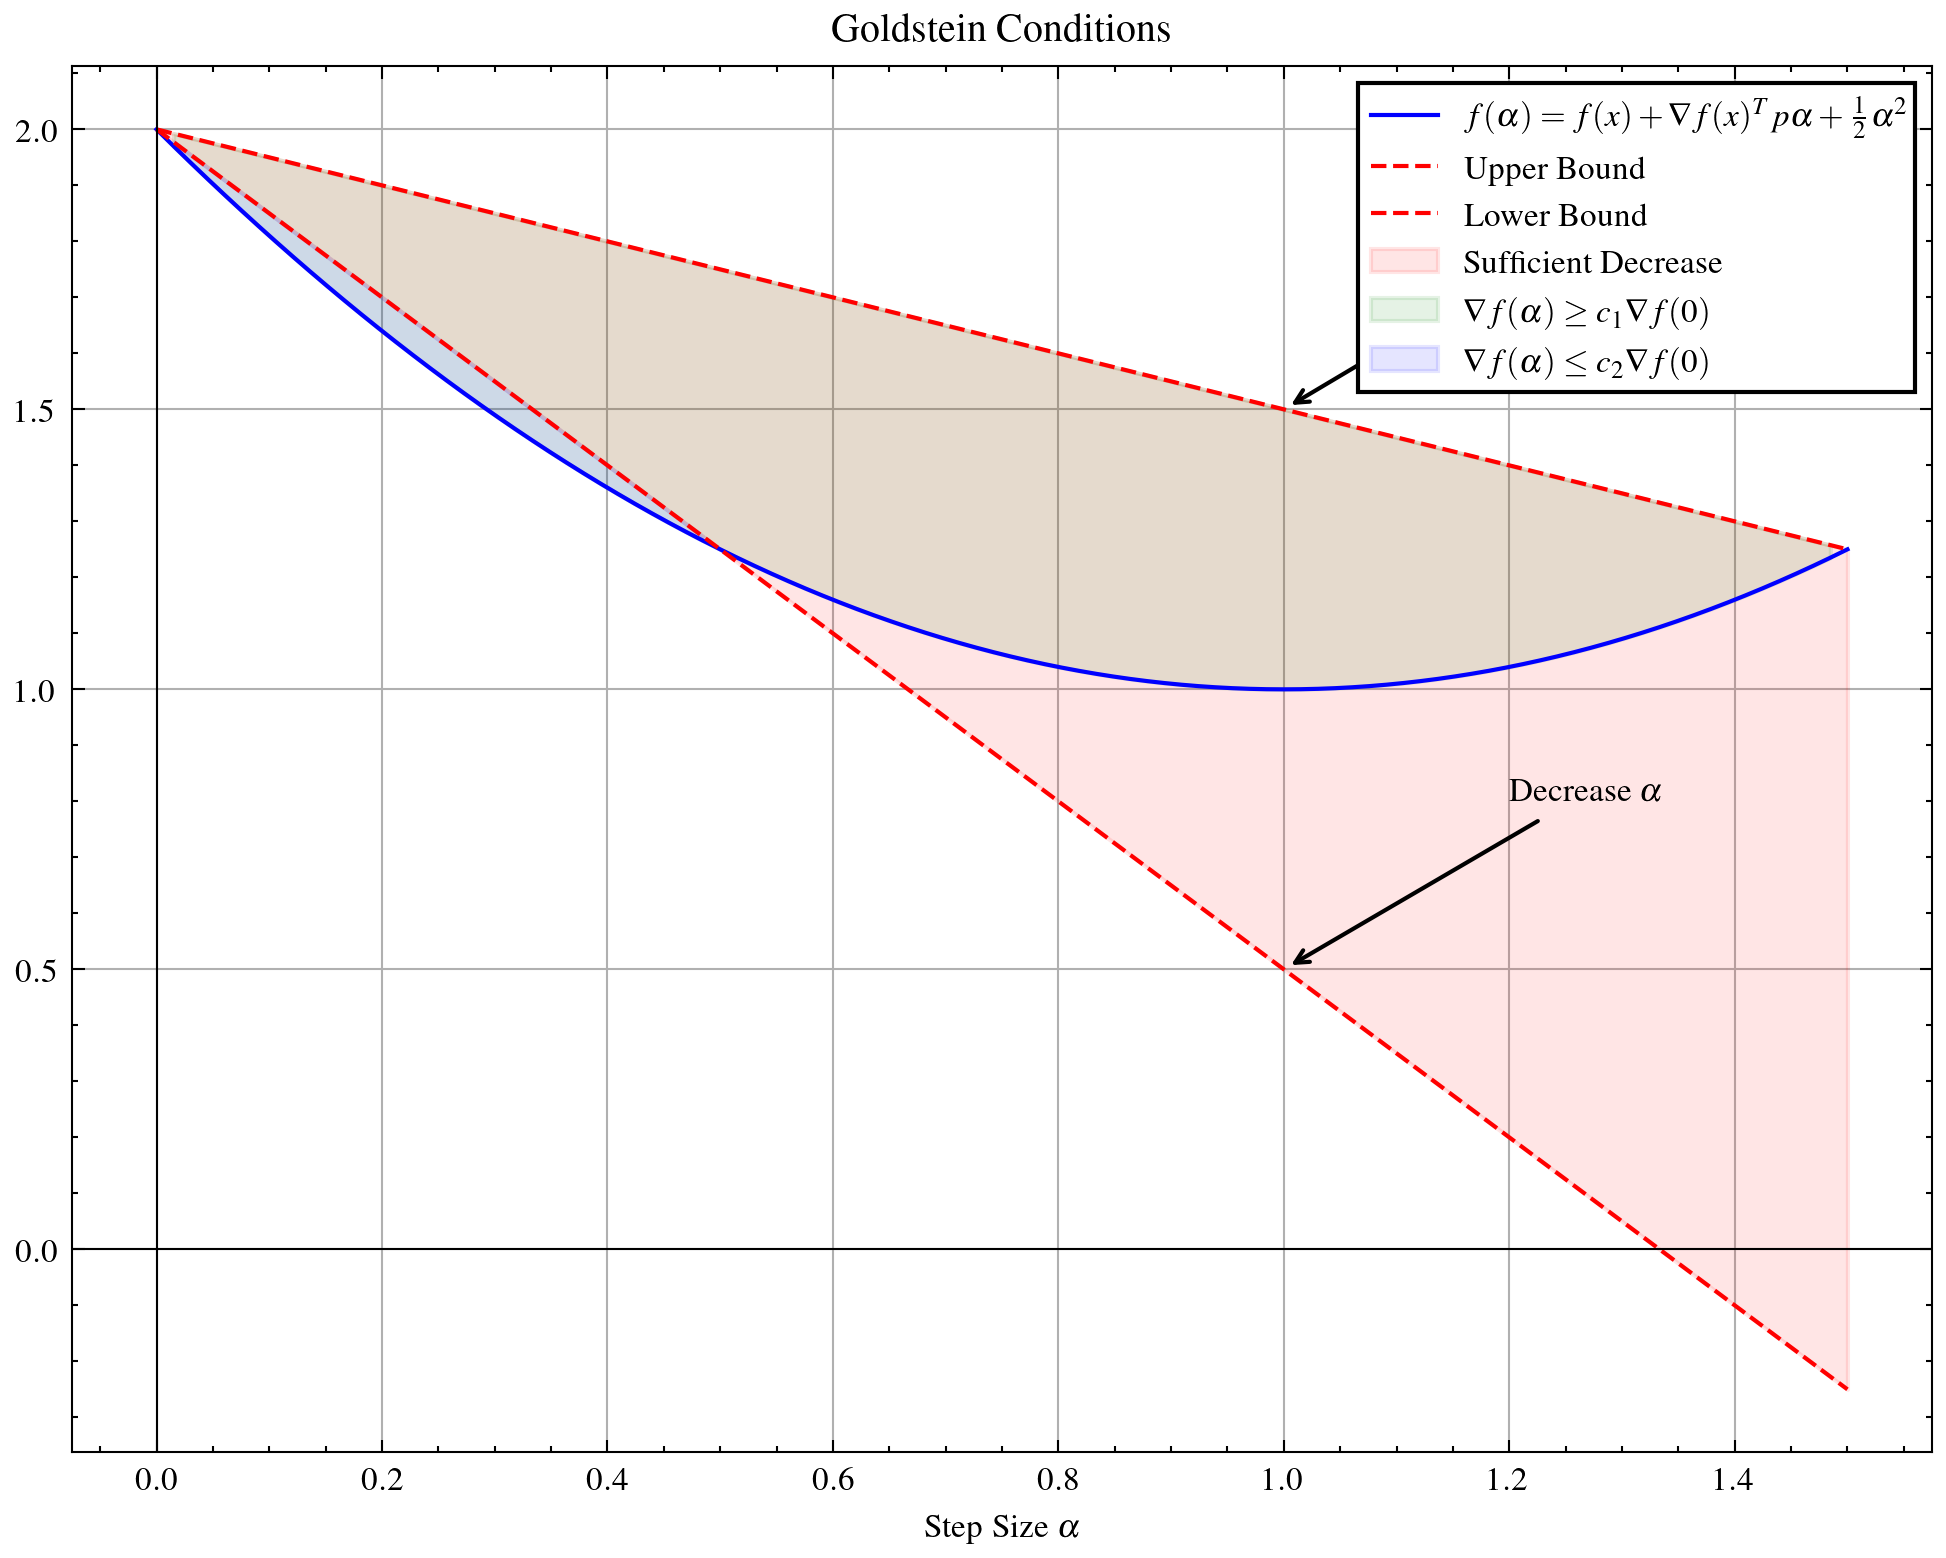
\includegraphics[scale=0.5]{figures/goldstein_conditions.png}
\begin{itemize}
  \item \textbf{Sufficient decrease:}  \(f(x_k + \alpha p_k) \leq f(x_k) + c_1 \alpha \inner{\nabla f(x_k), p_k}\). If this fails, decrease  \(\alpha\) because it is too large.
  \item \textbf{Curvature condition:}  \(f(x_k + \alpha p_k) \geq f(x_k) + c_2 \alpha \inner{\nabla f(x_k), p_k}\). If this fails, increase  \(\alpha\) because it is too small.
  \item Goldstein conditions are more robust than Armijo conditions.
\end{itemize}

\subsubsection*{Wolfe conditions}
Choose  \(0 < c_1 < c_2 < 1\).
\begin{itemize}
  \item \textbf{Sufficient decrease:}  \(f(x_k + \alpha p_k) \leq f(x_k) + c_1 \alpha \inner{\nabla f(x_k), p_k}\). If this fails, decrease  \(\alpha\) because it is too large.
  \item \textbf{Curvature condition:}  \(\inner{\nabla f(x_k + \alpha p_k)}{p_k} \geq c_2 \inner{\nabla f(x_k)}{p_k}\). If this fails, increase  \(\alpha\) because it is too small.
  \item Wolfe conditions are more robust than Goldstein conditions.
\end{itemize}

\section{Lecture 6 (24. Januar 2025)}
\subsection*{Backtracking Linjesøk}
Backtracking Line Search er en metode for å finne en passende skrittlengde \( \alpha \) i iterative optimeringsalgoritmer. Målet er å sikre at skrittet reduserer objektivfunksjonen \( f(\bm{x} + \alpha \bm{p}) \) tilstrekkelig, samtidig som det unngås for små eller ustabile skritt.

\subsubsection*{Algoritme og Matematisk Formulering}
La \( f: \R^n \to \R \) være kontinuerlig deriverbar, og \( \bm{p} \in \R^n \) en nedstigningsretning (dvs. \( \langle \nabla f(\bm{x}), \bm{p} \rangle < 0 \)). Algoritmen søker \( \alpha > 0 \) som tilfredsstiller \textbf{Armijo-betingelsen}:
\[
  f(\bm{x} + \alpha \bm{p}) \leq f(\bm{x}) + c_1 \alpha \langle \nabla f(\bm{x}), \bm{p} \rangle, \quad c_1 \in (0, 1).
\]

\begin{algorithm}[H]
  \SetAlgoLined
  \DontPrintSemicolon
  \KwIn{ \(\alpha_0 > 0\),  \(c_1 \in (0,1)\),  \(\rho \in (0,1)\)}
  \KwOut{ \(\alpha\)}
  \(\alpha \leftarrow \alpha_0\)\;
  \While{ \(f(\bm{x} + \alpha \bm{p}) > f(\bm{x}) + c_1 \alpha \langle \nabla f(\bm{x}), \bm{p} \rangle\)}{
    \(\alpha \leftarrow \rho \alpha\) \tcp*{Reduser skrittlengde}
  }
  \Return{ \(\alpha\)}
  \caption{Backtracking Linjesøk (Armijo)}
\end{algorithm}

\subsubsection*{Relaterte Betingelser}
\begin{itemize}
  \item \textbf{Armijo-Goldstein}: Legger til en nedre grense for \( \alpha \):
        \[
          f(\bm{x}) + c_2 \alpha \langle \nabla f(\bm{x}), \bm{p} \rangle \leq f(\bm{x} + \alpha \bm{p}) \leq f(\bm{x}) + c_1 \alpha \langle \nabla f(\bm{x}), \bm{p} \rangle, \quad 0 < c_1 < c_2 < 1.
        \]

  \item \textbf{Wolfe-betingelsene}: Inkluderer krumningstilstand:
        \[
          \langle \nabla f(\bm{x} + \alpha \bm{p}), \bm{p} \rangle \geq c_2 \langle \nabla f(\bm{x}), \bm{p} \rangle, \quad 0 < c_1 < c_2 < 1.
        \]
\end{itemize}

\begin{lemma}{Terminering}{}
  Hvis \( f \in C^2 \) er nedre begrenset og \( \bm{p} \) er en nedstigningsretning, terminerer backtracking-algoritmen med en endelig \( \alpha > 0 \).
\end{lemma}

\begin{theorem}{Konvergens for Gradient Descent}{}
  Anta:
  \begin{itemize}
    \item \( f \in C^2 \) med kompakt nivåmengde \( \mathcal{L}_f(\bm{x}_0) = \{\bm{x} \in \R^n \mid f(\bm{x}) \leq f(\bm{x}_0)\} \)
    \item \( \bm{p}_k = -\nabla f(\bm{x}_k) \)
    \item \( \alpha_k \) tilfredsstiller Armijo- eller Wolfe-betingelsene
  \end{itemize}
  Da gjelder:
  \[
    \lim_{k \to \infty} \|\nabla f(\bm{x}_k)\| = 0.
  \]
\end{theorem}

\begin{example}{Kvadratisk Funksjon}{}
  For \( f(\bm{x}) = \frac{1}{2} \bm{x}^\top Q \bm{x} - \bm{b}^\top \bm{x} \) med \( Q \succ 0 \), gir eksakt linjesøk:
  \begin{align*}
    \alpha_k                          & = -\frac{\langle \bm{p}_k, \nabla f(\bm{x}_k) \rangle}{\langle \bm{p}_k, Q \bm{p}_k \rangle}, \\
    \|\bm{x}_{k+1} - \bm{x}^\star\|_Q & \leq \frac{\kappa - 1}{\kappa + 1} \|\bm{x}_k - \bm{x}^\star\|_Q,
  \end{align*}
  hvor \( \kappa = \operatorname{cond}(Q) = \frac{\lambda_{\max}(Q)}{\lambda_{\min}(Q)} \).
\end{example}

\begin{example}{Rosenbrock-funksjonen: Hessian}{}
  For \( f(x,y) = (1 - x)^2 + 100(y - x^2)^2 \) har Hessianen i minimum \( \bm{x}^\star = (1,1) \) formen:
  \[
    H_f(1,1) = \begin{bmatrix} 802 & -400 \\ -400 & 200 \end{bmatrix}.
  \]
  Kondisjonstallet \( \kappa \approx 2500 \) forklarer treg konvergens for gradientdescent.
\end{example}

\section{Lecture 7 (27. Januar 2025)}

\subsection*{Goal for today}
\begin{itemize}
  \item Newton's Method:
        \begin{itemize}
          \item Definition and convergence rate
          \item Combination with line search
          \item Necessary modifications
        \end{itemize}
\end{itemize}

\subsection*{Newton's Method}

\subsection*{Background}
Assume \(G: \R^d \to \R^d\). We want to solve \(G(x) = 0\).

Newton's method is an iterative procedure for finding the roots of a differentiable function \(G: \R^d \to \R^d\).
It uses the first-order Taylor (linear) approximation of \(G\) at the current point \(x_k\).

\begin{definition}{Newton's Method}{}
  The iteration is defined by
  \begin{align*}
    x_{k+1} & = x_k - \bigl(D G(x_k)\bigr)^{-1} G(x_k),
  \end{align*}
  where \(D G(x_k)\) is the derivative (Jacobian) of \(G\) at \(x_k\). If \(G\) is the gradient of a scalar function \(f\), then \(DG(x_k) = H_f(x_k)\), the Hessian of \(f\).
\end{definition}

\subsection*{Convergence Theory}
If \(G\in \mathcal{C}^2\), then this iteration converges locally \emph{quadratically} to
a solution \(x^\star\) of \(G(x) = 0\), provided that \(D G(x^\star)\) is invertible.

\begin{remark}
  Quadratic convergence means there exist constants \(C>0\) and \(\delta>0\) such that for all \(k\) with \(\|x_k - x^\star\|\le \delta\),
  \[
    \|x_{k+1} - x^\star\| \;\le\; C \,\|x_k - x^\star\|^2.
  \]
\end{remark}

\subsubsection*{Application to Optimization}

We apply Newton's method to solve \(\nabla f(x) = 0\). That is, to find stationary points of a function \(f:\R^d \to \R\).

\subsection*{Basic Method}
\begin{itemize}
  \item Newton iteration:
        \[
          x_{k+1} \;=\; x_k \;-\; H_f(x_k)^{-1} \,\nabla f(x_k).
        \]
  \item Alternatively, set up the system \(H_f(x_k)\,p_k = -\,\nabla f(x_k)\) and then \(x_{k+1} = x_k + p_k\).
  \item Convergence: If \(f\in \mathcal{C}^3\) and \(H_f(x^\star)\) is nonsingular at the local minimizer \(x^\star\), the method converges locally quadratically.
\end{itemize}

\begin{algorithm}[H]
  \caption{Basic Newton's Method}
  \label{alg:newton-basic}
  \KwInput{Starting point  \(x_0\), tolerance  \(\epsilon > 0\)}
  \KwOutput{Approximate solution  \(x_k\)}
  \(k \gets 0\)\;
  \While{ \(\|\nabla f(x_k)\| > \epsilon\)}{
    Compute Hessian  \(H_f(x_k)\)\;
    Solve  \(H_f(x_k)\,p_k = -\,\nabla f(x_k)\)\;
    \(x_{k+1} \gets x_k + p_k\)\;
    \(k \gets k + 1\)\;
  }
  \KwRet{ \(x_k\)}\;
\end{algorithm}

\subsection*{Global Convergence Strategy}
\begin{enumerate}
  \item Combine with a line search.
  \item Define \(p_k\) by solving \(H_f(x_k)\,p_k = -\nabla f(x_k)\).
  \item Choose a step length \(\alpha_k > 0\).
  \item Update \(x_{k+1} = x_k + \alpha_k \, p_k\).
\end{enumerate}

\begin{algorithm}[H]
  \caption{Globally Convergent Newton's Method}
  \label{alg:newton-global}
  \KwInput{Starting point  \(x_0\), tolerances  \(\epsilon, c > 0\), reduction factor  \(\rho \in (0,1)\)}
  \KwOutput{Approximate solution  \(x_k\)}
  \(k \gets 0\)\;
  \While{ \(\|\nabla f(x_k)\| > \epsilon\)}{
    Compute Hessian  \(H_f(x_k)\)\;
    Solve  \(H_f(x_k)\,p_k = -\nabla f(x_k)\)\;
    \(\alpha_k \gets 1\)\;
    \While{ \(f(x_k + \alpha_k p_k) > f(x_k) + c\,\alpha_k\,\nabla f(x_k)^\top p_k\)}{
      \(\alpha_k \gets \rho\,\alpha_k\)\;
    }
    \(x_{k+1} \gets x_k + \alpha_k p_k\)\;
    \(k \gets k + 1\)\;
  }
  \KwRet{ \(x_k\)}\;
\end{algorithm}

\subsection*{Descent Direction Condition}
If \(H_f(x_k)\) is positive definite, then
\[
  \langle p_k, \nabla f(x_k)\rangle
  \;=\;
  -\,\langle H_f(x_k)^{-1}\,\nabla f(x_k),\,\nabla f(x_k)\rangle
  \;<\; 0,
\]
so \(p_k\) is a descent direction for the line search.

\subsection*{Modified Newton's Method}
If \(H_f(x_k)\) is not positive definite, or if \(\langle \nabla f(x_k), p_k\rangle \geq 0\), then the line search may fail. One approach is to modify the Hessian or switch to a different direction:

\begin{itemize}
  \item First compute \(p_k = -\,H_f(x_k)^{-1}\,\nabla f(x_k)\).
  \item If \(\langle \nabla f(x_k),\,p_k\rangle \;\ge\; \varepsilon \,\|\nabla f(x_k)\|\,\|p_k\|\) for some \(\varepsilon > 0\), switch to \(p_k = -\,\nabla f(x_k)\).
  \item Alternatively, modify the Hessian so it is sufficiently positive definite (e.g.\ shift its eigenvalues).
\end{itemize}

\begin{algorithm}[H]
  \caption{Modified Newton's Method with Hessian Modification}
  \label{alg:newton-modified}
  \KwInput{Starting point  \(x_0\), tolerances  \(\epsilon, \varepsilon > 0\)}
  \KwOutput{Approximate solution  \(x_k\)}
  \(k \gets 0\)\;
  \While{ \(\|\nabla f(x_k)\| > \epsilon\)}{
  Compute Hessian  \(H_f(x_k)\)\;
  Compute eigendecomposition  \(H_f(x_k) = U\,\Lambda\,U^\top\)\;
  \(M \gets \text{diag}\bigl(\max\{\lambda_1, \varepsilon\}, \ldots, \max\{\lambda_d, \varepsilon\}\bigr)\)\;
  \(p_k \gets -\,U\,M^{-1}\,U^\top\,\nabla f(x_k)\)\;
  \uIf{ \(\nabla f(x_k)^\top p_k < -\,\varepsilon\,\|\nabla f(x_k)\|\|p_k\|\)}{
    Use  \(p_k\) as the search direction\;
  }
  \Else{
    \(p_k \gets -\,\nabla f(x_k)\)\;
  }
  % In a global method, we would then do a line search on p_k:
  %   x_{k+1} = x_k + alpha_k p_k
  % but here it is omitted for brevity.
  \(x_{k+1} \gets x_k + p_k\)\;
  \(k \gets k + 1\)\;
  }
  \KwRet{ \(x_k\)}\;
\end{algorithm}

\subsection*{Alternative Interpretation of Newton's Method}
Newton's method can also be viewed via a second-order Taylor expansion of \(f\) around \(x_k\):

\begin{enumerate}
  \item Approximate \(f\) by
        \[
          m_k(p) \;=\; f(x_k) \;+\; \langle \nabla f(x_k),\, p\rangle \;+\; \tfrac12\,\langle H_f(x_k)\,p,\,p\rangle.
        \]
  \item Find \(p_k\) by minimizing \(m_k(p)\).
        \[
          \nabla m_k(p_k) \;=\; \nabla f(x_k) \;+\; H_f(x_k)\,p_k \;=\; 0
          \quad\Longrightarrow\quad
          p_k = -\,H_f(x_k)^{-1}\,\nabla f(x_k).
        \]
  \item If \(H_f(x_k)\) is not positive definite, one modifies it to be positive definite (e.g.\ shifting eigenvalues).
\end{enumerate}

The \emph{modified Newton's method} then reads \(x_{k+1} = x_k + \alpha_k\,p_k\) with \(\alpha_k>0\) found by a line search and \(p_k\) given by one of the strategies above.

\subsection*{Quadratic Convergence Criterion}
Quadratic convergence holds precisely when, near \(x^\star\), we use
\[
  p_k \;=\; -\,H_f(x_k)^{-1}\,\nabla f(x_k)
  \quad\text{and}\quad
  \alpha_k \;=\; 1.
\]
In particular, for \(\alpha_k = 1\) to be acceptable in the line search once \(x_k\) is close to \(x^\star\), the Hessian near \(x^\star\) must be uniformly positive definite (so all eigenvalues \(\ge \varepsilon > 0\)), and the line search parameters (e.g.\ the Armijo or Wolfe constants) must allow a full step.

\subsection*{Conjugate Gradient Methods}

We now focus on the special case of minimizing the quadratic function
\[
  \Phi(x) \;:=\; \tfrac12\,\langle x,\;Q\,x\rangle \;-\; \langle b,\;x\rangle,
\]
where \(Q \in \R^{d\times d}\) is symmetric positive definite and \(b \in \R^d\). In exact arithmetic, the \emph{Conjugate Gradient} (CG) method can solve this problem in at most \(d\) steps.

With exact line search, the update is
\[
  x_{k+1}
  \;=\; x_k \;-\; \frac{\langle Q\,x_k - b,\;p_k\rangle}{\langle Q\,p_k,\;p_k\rangle}\,p_k,
\]
which ensures
\[
  \langle \nabla \Phi(x_{k+1}),\;p_k\rangle \;=\; 0.
\]
In particular, for a gradient method we would have \(\nabla \Phi(x_{k+1}) \propto p_{k+1}\). Orthogonality conditions arise naturally here.

\subsection*{Conjugate Directions}
A set of vectors \(\{p_0, p_1, \dots, p_{d-1}\}\subset \R^d\) is \emph{conjugate} with respect to \(Q\) if
\[
  \langle p_i,\;Q\,p_j\rangle \;=\; 0 \quad\text{for}\quad i\neq j.
\]
Equivalently, the vectors are mutually orthogonal under the inner product \(\langle u, v \rangle_Q := \langle u, Q\,v\rangle\).

\begin{lemma}{Conjugate Directions}{}
  Let \(\{p_0,\ldots,p_{d-1}\}\) be a conjugate basis of \(\R^d\). Consider the iteration
  \[
    x_{k+1} \;=\; x_k + \alpha_k\,p_k
    \quad\text{with}\quad
    \alpha_k \;=\; -\,\frac{\langle r_k,\;p_k\rangle}{\langle Q\,p_k,\;p_k\rangle},
  \]
  where \(r_k = Q\,x_k - b\). Then \(x_d = x^\star = Q^{-1}b\). In other words, the exact solution is reached in at most \(d\) steps.
\end{lemma}

\begin{proof}{}{}
  Since \(\{p_0,\ldots,p_{d-1}\}\) is a basis, there exist scalars \(\sigma_k\) such that
  \[
    x^\star - x_0
    \;=\; \sum_{k=0}^{d-1} \sigma_k\,p_k.
  \]
  Also,
  \[
    x_d - x_0
    \;=\; \sum_{k=0}^{d-1} \alpha_k\,p_k.
  \]
  To show \(x_d = x^\star\), it suffices to prove \(\sigma_k = \alpha_k\) for all \(k\). Indeed,
  \[
    \sigma_l
    \;=\; \frac{\langle x^\star - x_0,\;Q\,p_l\rangle}{\langle p_l,\;Q\,p_l\rangle}
    \;=\; \frac{\langle Q\,(x^\star - x_0),\;p_l\rangle}{\langle p_l,\;Q\,p_l\rangle}
    \;=\; \frac{\langle b - Q\,x_0,\;p_l\rangle}{\langle p_l,\;Q\,p_l\rangle}.
  \]
  Also,
  \[
    \alpha_l
    \;=\; -\,\frac{\langle r_0,\;p_l\rangle}{\langle Q\,p_l,\;p_l\rangle},
    \quad\text{where}\quad r_0 \;=\; Q\,x_0 - b.
  \]

  Careful manipulation (and using the fact that \(\langle p_i, Q\,p_j\rangle=0\) for \(i\neq j\)) shows \(\sigma_l = \alpha_l\). Hence \(x^\star = x_d\).

\end{proof}

\subsection*{The CG Iteration}
The Conjugate Gradient method constructs a sequence of conjugate directions by choosing
\[
  p_0 = -\,r_0 \;=\; b - Q\,x_0,
  \quad
  p_{k+1} = -\,r_{k+1} + \beta_k\,p_k
\]
with \(\beta_k\) chosen so that \(\langle p_{k+1},\,Q\,p_k\rangle=0\). One can show this leads to convergence in at most \(d\) steps for solving \(Q\,x = b\) in exact arithmetic.

\section{Lecture 8 (31. February 2025)}

\textbf{Goals:}
\begin{enumerate}
  \item \textbf{CG Convergence:} Theoretical guarantees and convergence speed
  \item \textbf{Efficient Reformulation:} Practical CG improvements
  \item \textbf{Nonlinear Extension:} Fletcher--Reeves method
  \item \textbf{Step Length Selection:} Optimal step size strategies
  \item \textbf{Alternative Methods:} Polak--Ribière and Hestenes--Stiefel variants
\end{enumerate}

\begin{theorem}{}{}
  As long as \(r_k \neq 0\), we have that:
  \begin{itemize}
    \item \(\inner{r_k, r_e}=0 \forall l = 0,...,k-1 \)
    \item \(\spann\{p_0,\ldots, p_k\} = \spann\{r_0, \ldots, r_k\} = \spann\{r_0, Qr_0, Q^2r_0,\ldots, Q^k r_0\}\)
    \item \(\inner\{p_k, Qp_l\} = 0 \forall \; l=0,\ldots,k-1\)
    \item In particular
  \end{itemize}
\end{theorem}

\begin{lemma}{}{}
  Assume that \(\alpha\) satisfies in each step the strong curvature condition:
  \[
    \left|\inner{}\right|
  \]
\end{lemma}

\section{Lecture 9 \emph{3. Februar 2025}}

\begin{definition}{Newton's Method}{newton-method}
  \[
    x_{k+1} = x_k - [\nabla^2 f(x_k)]^{-1} \nabla f(x_k) = x_k - H_k^{-1} \nabla f(x_k) = x_k + p_k
  \]
  where \( H_k \) is the Hessian matrix.
\end{definition}

But computing the Hessian matrix is expensive, so we use the \textbf{quasi-Newton} method instead.

\subsection*{Quasi-Newton Methods}
The quasi-Newton method is an iterative optimization algorithm that approximates the Hessian matrix using rank-one updates.
This approach avoids the computational cost of computing the exact Hessian matrix and can provide faster convergence rates.
\begin{definition}{Quasi-Newton Method}{quasi-newton}
  \[
    x_{k+1} = x_k - B_k^{-1} \nabla f(x_k) = x_k + p_k
  \]
  where \( B_k \) is an approximation of the Hessian matrix.
\end{definition}

\begin{algorithm}[H]
  \caption{Quasi-Newton Method}
  \label{alg:quasi-newton}
  \SetKwFunction{QuasiNewton}{QuasiNewton}
  \QuasiNewton{ \(x_0\),  \(B_0\),  \(f\),  \(\nabla f\),  \(\epsilon\)}\;
  \While{ \(\norm{\nabla f(x_k)} > \epsilon\)}{
  Compute the search direction  \(p_k = -B_k^{-1} \nabla f(x_k)\)\;
  Choose the step size  \(\alpha_k\) by line search\;
  Update the current point  \(x_{k+1} = x_k + \alpha_k p_k\)\;
  Update the approximation  \(B_{k+1}\) of the Hessian matrix\;
  }
  \KwRet{ \(x_k\)}\;
\end{algorithm}

\subsubsection*{Update Formulas}

\begin{itemize}
  \item \textbf{DFP update}: \( B_{k+1} = B_k + \frac{y_k y_k^T}{y_k^T s_k} - \frac{B_k s_k s_k^T B_k}{s_k^T B_k s_k} \)
  \item \textbf{BFGS update}: \( B_{k+1} = B_k + \frac{(y_k y_k^T)}{y_k^T s_k} - \frac{(B_k s_k)(B_k s_k)^T}{s_k^T B_k s_k} \)
  \item \textbf{SR1 update}: \( B_{k+1} = B_k + \frac{(y_k - B_k s_k)(y_k - B_k s_k)^T}{(y_k - B_k s_k)^T s_k} \)
  \item \textbf{Broyden update}: \( B_{k+1} = B_k + \frac{(y_k - B_k s_k - B_k^T y_k)(s_k^T B_k)}{s_k^T B_k s_k} \)
\end{itemize}

\subsubsection*{SR1 Update}
The SR1 update is a rank-one update that approximates the Hessian matrix using the following formula:
\[
  B_{k+1} = B_k + \frac{(y_k - B_k s_k)(y_k - B_k s_k)^T}{(y_k - B_k s_k)^T s_k}
\]
where \( s_k = x_{k+1} - x_k \) and \( y_k = \nabla f(x_{k+1}) - \nabla f(x_k) \).

\clearpage

\section{Lecture 10 \emph{7. Februar 2025}}

\subsection*{Læringsmål}
\begin{enumerate}
  \item \textbf{Quasi-Newton Methods}
  \item BFGS
  \item DFP
\end{enumerate}

\subsection*{Fra tidligere: Quasi-Newton Metoder}
\begin{align*}
  p_k     & = -B_k^{-1} \nabla f(x_k) = -H_k^{-1} \nabla f(x_k) \\
  x_{k+1} & = x_k + \alpha_k p_k                                \\
  B_{k+1} & = B_k + \text{update}
\end{align*}

\paragraph{DFP oppdatering: Regne ut \(B_{k+1}\)}
\begin{itemize}
  \item \textbf{Symmetrisk}
  \item \textbf{Sekantligning}: \(B_{k+1} s_k = y_k\) med \(s_k = x_{k+1} - x_k\) og \(y_k = \nabla f(x_{k+1}) - \nabla f(x_k)\).
  \item \(B_{k+1}\) er nærme \(B_k\) og tilfredsstiller sekantligningen.
\end{itemize}

Nytt: tolk "nærme" som minimeringen av en norm.

Definer \( B_{k+1} \) som løsning til
\[
  \min_{B \in \R^{d \times d}} \frac{1}{2} \norm{B - B_k}_F^2 \quad \text{s.a.} \quad B = B^T, \quad B s_k = y_k
\]

Valg av norm: Frobeniusnormen
\[
  G := \int_0^1 H_f(x_k + \tau \alpha p_k) \, d\tau
\]
Definerer en form for gjennomsnittlig Hessian av \( f \) langs linjen \([x_k, x_{k+1}]\).

La \( W = G^{-1} \) (der \( G \) er invertibel).

Definerer \( \norm{A}_W = \norm{WA}_F = \sqrt{\sum_{i,j} (W A)_{ij}^2} \).

\begin{remark}{}{}
  \begin{align*}
    Gs_k & = G(x_{k+1} - x_k) = G(\alpha p_k)                                                                                                                 \\
         & = \int_0^1 \overbrace{H_f(x_k + \tau \alpha p_k) \alpha p_k}^{\frac{\partial}{\partial \tau}\left[\nabla f(x_k + \tau \alpha p_k)\right]} \, d\tau \\
         & = \nabla f(x_k + \alpha p_k) - \nabla f(x_k) = y_k \quad \implies \quad Gs_k = y_k \quad \text{og} \quad W y_k = s_k
  \end{align*}
\end{remark}

\begin{theorem}{}{}
  Assume \(W\in \R^{d \times d}\) is symmetric positive definite, non-singular, and \(W y_k = s_k\). Then the solution to
  \[
    \min_{B \in \R^{d \times d}} \frac{1}{2} \norm{B - B_k}_W^2 \quad \text{s.a.} \quad B = B^T, \quad B s_k = y_k
  \]
  is given by
  \[
    B_{k+1} = \left(I - \rho_k y_k \otimes s_k\right) B_k \left(I - \rho_k s_k \otimes y_k\right) + \rho_k y_k \otimes y_k
  \]
  where \( \rho_k = \frac{1}{\inner{y_k, s_k}} \).

  This is the Davidon-Fletcher-Powell method (DFP).
\end{theorem}

\hrule
\vspace{1em}

\subsection*{BFGS oppdatering (Broyden-Fletcher-Goldfarb-Shanno)}

One can again work with \(H_k = B_k^{-1}\) instead.
Here we obtain the update formula:
\[
  H_{k+1} = H_k - \frac{\left(H_k y_k\right) \otimes \left(H_k y_k\right)}{\inner{y_k, H_k y_k}} + \frac{s_k \otimes s_k}{\inner{y_k, s_k}}
  = H_k + \frac{(s_k - H_k y_k)(s_k - H_k y_k)^T}{\inner{y_k, s_k}}
\]

Alternativt kan vi starte direkte med \(H_k \):

Definerer \( H_{k+1} \) med å minimere \( \norm{H - H_k}_G \) s.a. \( H = H^T \) og \( H y_k = s_k \).
Da får vi Broyden-Fletcher-Goldfarb-Shanno (BFGS) metoden.

\[
  H_{k+1} = H_k + \left(I - \rho_k s_k \otimes y_k\right) \left(I - \rho_k y_k \otimes s_k\right) + \rho_k s_k \otimes s_k \quad \text{med} \quad \rho_k = \frac{1}{\inner{s_k, y_k}}
\]

\begin{lemma}{}{}
  Anta at \( H_k \) er positiv definit og kan finnes med \textit{BFGS} eller \textit{DFP} oppdateringer.
  Hvis \( \inner{y_k, s_k} > 0 \), så er \( H_{k+1} \) positiv definit.
\end{lemma}

\begin{proof}{BFGS}{}
  La \( z \in \R^d \backslash \{0\} \) være en vilkårlig vektor.
  Da er:
  \begin{align*}
    \inner{z, H_{k+1} z} & = \inner{z, H_k z} + \inner{z, \left(I - \rho_k s_k \otimes y_k\right)H_k \left(I - \rho_k y_k \otimes s_k\right) z} + \rho_k \inner{z, \left(s_k \otimes s_k\right) z}   \\
                         & = \inner{\overbrace{\left(I - \rho_k y_k \otimes s_k\right) z}^{w}, H_k \overbrace{\left(I - \rho_k s_k \otimes y_k\right) z}^{w}} + \rho_k \inner{z, \inner{s_k, z} s_k} \\
                         & = \inner{w, H_k w} + \rho_k \inner{s_k, z}^2 \geq 0 \quad \text{og} \quad \inner{z, H_{k+1} z} = 0 \iff \inner{s_k, z} = 0, \quad w = 0
  \end{align*}
  Nå er \( w = \left(I - \rho_k y_k \otimes s_k\right) z = z - \rho_k \inner{y_k, z} s_k \), så hvis \( \inner{s_k, z} = 0 \) så er \( w = z \neq 0 \).
  Dermed er enten \( \rho_k\inner{y_k, z}^2\) eller \( \inner{w, H_k w} \) positiv, så \(\implies H_{k+1} \) er positiv definit.

  \qed
\end{proof}


Hvis vi kan garantere at \( \inner{y_k, s_k} \gg 0 \; \forall k \) og \( H_0 \) er positiv definit, så vil \( H_{k+1} \) være positiv definit for alle \( k \), og \(p_{k+1} = -H_{k+1} \nabla f(x_k) \) vil være en nedstigningsretning.

Hvis \( f \) er strengt konveks (og dermed \(x_{k+1} \neq x_k \) for alle \( k \)), så vil

\[
  \inner{\nabla f(x_{k+1}) - \nabla f(x_k), x_{k+1} - x_k} > 0
\]

\begin{itemize}
  \item Anta at \(\alpha_k\) er valgt mhp Wolfe-betingelsene. Da er
        \[
          \inner{\nabla f(x_k + \alpha_k p_k), p_k} \geq c_2 \inner{\nabla f(x_k), p_k} \quad \text{og} \quad \inner{\nabla f(x_{k+1}), p_k} \geq c_1 \inner{\nabla f(x_k), p_k}
        \]
  \item Implementer BFGS/DFP oppdateringene med linjesøk (Wolfe-betingelsene) og velg \( H_0 \) positiv definit.
        \[
          H_0 = c \, I \quad \text{hvor} \quad c > 0
        \]

  
  \item \textbf{Vanlig strategi:} Først velg \( p_0 = -\nabla f(x_0) \) og finn \( \alpha_0 \) med linjesøk (f.eks. Wolfe-betingelsene).
  \item Deretter finner vi \(x_1 = x_0 + \alpha_0 p_0 \) og \( s_0 = x_1 - x_0 \) og \( y_0 = \nabla f(x_1) - \nabla f(x_0) \).
  \item Definerer så \( c = \frac{\inner{y_0, s_0}}{\inner{y_0, y_0}} \) og \( H_0 = c \, I \).
  \item Regn ut \( H_1 = H_0 + \text{BFGS/DFP update} \).
\end{itemize}

\begin{figure}[H]
  \begin{minipage}[t]{0.49\textwidth}
    \begin{algorithm}[H]
      \caption{BFGS + Wolfe Conditions}
      \label{alg:bfgs}
      \KwIn{Initial point \(x_0\), tolerance \(\epsilon>0\), \(N\), \(H_0 = I\)}
      \For{\(k=0,1,\ldots,N\)}{
        Compute \(g_k = \nabla f(x_k)\)\;
        \If{\(\|g_k\| < \epsilon\)}{
          \Return{\(x_k\)}\;
        }
        Set \(p_k = -H_k g_k\)\;
        Find step size \(\alpha_k\) via Wolfe line search\;
        Update \(x_{k+1} = x_k + \alpha_k p_k\)\;
        Set \(s_k = x_{k+1} - x_k\)\;
        Set \(y_k = \nabla f(x_{k+1}) - g_k\)\;
        Set \(\rho_k = \frac{1}{y_k^\top s_k}\)\;
        Update inverse Hessian: \(H_{k+1} = (I - \rho_k s_k y_k^\top) H_k (I - \rho_k y_k s_k^\top) + \rho_k s_k s_k^\top\)
      }
      \Return{\(x_{k+1}\)}\;
    \end{algorithm}
  \end{minipage}
  \hfill
  \begin{minipage}[t]{0.49\textwidth}
    \begin{algorithm}[H]
      \caption{DFP with Wolfe Conditions}
      \label{alg:dfp}
      \KwIn{Initial point \(x_0\), tolerance \(\epsilon>0\), \(N\), \(B_0 = I\)}
      \For{\(k=0,1,\ldots,N\)}{
        Compute \(g_k = \nabla f(x_k)\)\;
        \If{\(\|g_k\| < \epsilon\)}{
          \Return{\(x_k\)}\;
        }
        Solve \(B_k p_k = -g_k\) for \(p_k\)\;
        Find step size \(\alpha_k\) via Wolfe line search\;
        Update \(x_{k+1} = x_k + \alpha_k p_k\)\;
        Set \(s_k = x_{k+1} - x_k\)\;
        Set \(y_k = \nabla f(x_{k+1}) - g_k\)\;
        Set \(\rho_k = \frac{1}{y_k^\top s_k}\)\;
        Update Hessian: \(B_{k+1} = (I - \rho_k y_k s_k^\top) B_k (I - \rho_k s_k y_k^\top) + \rho_k y_k y_k^\top\)
      }
      \Return{\(x_{k+1}\)}\;
    \end{algorithm}
  \end{minipage}
\end{figure}

\section{Lecture 11 \emph{10. Februar 2025}}

\subsection*{Læringsmål}
\begin{enumerate}
  \item Optimisation with convex constraints
  \item Various formulations of optimality conditions
  \item Feasible directions, tangent cones and normal cones
  \item Projections onto convex sets
  \item Projected gradient descent
\end{enumerate}

\subsection*{Optimalisering med konvekse begrensninger}
\begin{itemize}
  \item \textbf{Problem:} Minimer \(\min_{\Omega \subset \R^d} f(x)\) hvor \(\Omega\) er konveks og lukket, med \(f: \R^d \to \R\) hvor \(f\in \mathcal{C}^1\).
  \item \textbf{Optimalitetsbetingelser:} Hvis \(x^\star\) løser problemet, så er det nødvendig at \(\nabla f(x^\star) = 0\) og \(x^\star \in \Omega\).
\end{itemize}

\begin{example}{\(f(x,y)=x, \quad \Omega = \{(x,y) \in \R^2 \mid x^2 + y^2 \leq 1\}\)}{}
  \begin{itemize}
    \item \textbf{Optimalitetsbetingelser:} \(\nabla f(x,y) = (1,0)\) og \((1,0) \in \Omega\).
    \item \textbf{Løsning:} \(x^\star = (1,0)\).
    \item La \((x^\star, y^\star)=(-1,0) \) og \(\nabla f(x^\star, y^\star) = (1,0)^T \). Observer at punktet peker mot settet \(\Omega\).
  \end{itemize}

  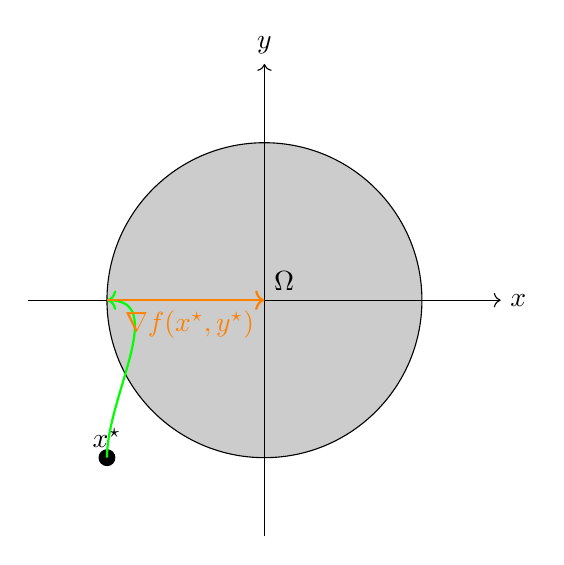
\begin{tikzpicture}[scale=2]
    \draw[fill=gray!40] (0,0) circle (1) node[above right] {\(\Omega\)};
    \draw[->] (-1.5,0) -- (1.5,0) node[right] {\(x\)};
    \draw[->] (0,-1.5) -- (0,1.5) node[above] {\(y\)};
    \draw[fill=black] (-1,-1) circle (0.05) node[above] {\(x^\star\)};
    \draw[->, thick, in=0, out=90, green] (-1,-1) to (-1, 0);
    \draw[->, thick, orange] (-1,0) -- (0,0) node[below left] {\(\nabla f(x^\star, y^\star)\)};
  \end{tikzpicture}

\end{example}


\begin{definition}{Bevegelse mot \(\Omega\)}{}
  La \(x \in \R^d\) og \(\Omega \subset \R^d\) være konveks og lukket.
  \begin{itemize}
    \item En vektor \(p \in \R^d\) er en \textbf{bevegelse mot \(\Omega\)} fra \(x\) hvis det finnes et \(\epsilon > 0\) slik at \(x + \tau p \in \Omega\) for alle \(\tau \in (0, \epsilon)\).
    \item La \(D(x)\) være mengden av alle bevegelser mot \(\Omega\) fra \(x\).
  \end{itemize}

  \[
    D(x) = \{p \in \R^d \mid \exists \epsilon > 0 \text{ slik at } x + \tau d \in \Omega \; \forall \tau \in (0, \epsilon)\}
  \]

\end{definition}

\begin{lemma}{}{}
  La \(\Omega \subseteq \R^d\) være konveks og lukket og \(x \in \Omega\).

  Da er \(p \in \R^d\) en bevegelse mot (feasible direction) \(\Omega\) fra \(x\) ekvivalent til

  \[
    \Leftrightarrow \exists \hat{x} \in \Omega \text{ og } t > 0 \text{ slik at } p = t(\hat{x} - x)
  \]

\end{lemma}

\begin{proposition}{}{}
  Anta at \(\Omega \subset \R^d\) er konveks og \(f: \R^d \to \R\) er i \(\mathcal{C}^1\).
  \begin{itemize}
    \item Hvis \(x^\star\) løser \(\min_{x \in \Omega} f(x)\), så er \(\inner{\nabla f(x^\star), p} \geq 0\) for alle mulige bevegelser til \(p\) ved \(x^\star\).
    \item Ekvivalent: \(\inner{\nabla f(x^\star), x - x^\star} \geq 0\) for alle \(x \in \Omega\).
    \item En konsekvens av at \(f\) er konveks og \(x^\star\) tilfredstiller betingelsen over, da er \(x^\star\) en global løsning for problemet \(\min_{x \in \Omega} f(x)\).
          \begin{proof}{}{}
            Anta at \(x^\star\) er en lokal løsning av (P) og \(p\) er en bevegelse mot \(\Omega\) fra \(x^\star\).
            \begin{align*}
              \exists t_0 > 0 \text{ s.a } x^\star + t_0 p \in \Omega \quad \text{og} \quad \Omega \text{ er konveks} \implies x^\star + t p \in \Omega \quad \forall t \in (0, t_0) \\
              x^\star \text{ er en lokal løsning av (P)} \implies \exists \varepsilon > 0 \text{ s.a } f(x^\star) \leq f(x^\star + t p) \quad \forall t \in (0, \varepsilon)         \\
              \implies \inner{\nabla f(x^\star), p} = \lim_{t \to 0^+} \frac{f(x^\star + t p) - f(x^\star)}{t} \geq 0                                                                \\
            \end{align*}

            Konvers: Anta at \(f\) er konveks og \(x^\star\) tilfredstiller betingelsen over. La \(x \in \Omega\), da får vi:
            \begin{align*}
              f(x) & \underbrace{\geq}_{\text{f er konveks.}} f(x^\star) + \underbrace{\inner{\nabla f(x^\star), x - x^\star}}_{\geq 0} \geq f(x^\star) \quad \forall x \in \Omega
            \end{align*}
            \qed
          \end{proof}
  \end{itemize}
\end{proposition}

\begin{definition}{}{}
  Anta at \(\Omega \subset \R^d\) er konveks og \(x \in \Omega\).

  Den normale kjeglen til \(\Omega\) ved \(x\) er gitt ved settet:
  \[
    N_\Omega(x) = \{p \in \R^d \mid \inner{p, y - x} \leq 0 \; \forall y \in \Omega\}
  \]

  Ekvivalent:
  \[
    q \in N_\Omega(x) \iff \inner{q, p} \leq 0 \; \forall p \in D(x)
  \]

  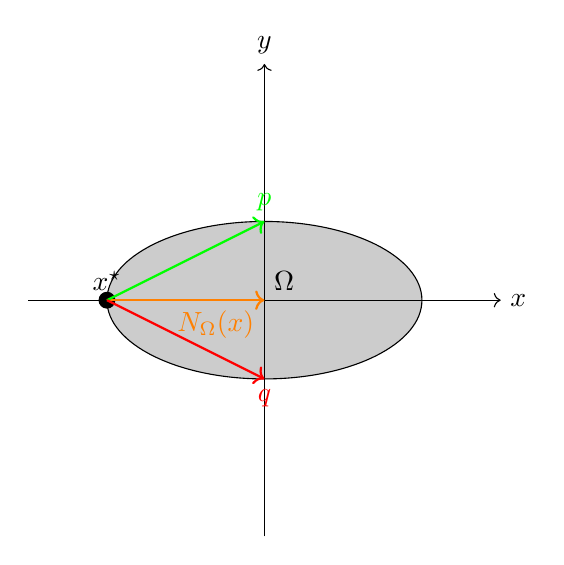
\begin{tikzpicture}[scale=2]
    \draw[fill=gray!40] (0,0) ellipse (1 and 0.5) node[above right] {\(\Omega\)};
    \draw[->] (-1.5,0) -- (1.5,0) node[right] {\(x\)};
    \draw[->] (0,-1.5) -- (0,1.5) node[above] {\(y\)};
    \draw[fill=black] (-1,0) circle (0.05) node[above] {\(x^\star\)};
    \draw[->, thick, orange] (-1,0) -- (0,0) node[below left] {\(N_\Omega(x)\)};
    \draw[->, thick, green] (-1,0) -- (0, 0.5) node[above] {\(p\)};
    \draw[->, thick, red] (-1,0) -- (0, -0.5) node[below] {\(q\)};
  \end{tikzpicture}
\end{definition}

\begin{proposition}{}{}
  Anta at \(\Omega \subset \R^d\) er konveks og \(x \in \Omega\).
  \begin{itemize}
    \item Hvis \(x^\star\) er en lokal løsning av (P) da er \(-\nabla f(x^\star) \in N_\Omega(x^\star)\).
    \item Konvers: Hvis \(f\) er konveks og \(-\nabla f(x^\star) \in N_\Omega(x^\star)\) da er \(x^\star\) en global løsning av (P).
  \end{itemize}

\end{proposition}
\begin{proof}{}{}
  \begin{align*}
    -\nabla f(x^\star) \in N_\Omega(x^\star) & \iff \inner{-\nabla f(x^\star), y - x^\star} \leq 0 \quad \forall y \in \Omega                \\
                                             & \iff f(y) \geq f(x^\star) + \inner{\nabla f(x^\star), y - x^\star} \quad \forall y \in \Omega
  \end{align*}
  \qed
\end{proof}
\begin{remark}{}{}
  Hvis \(x^\star \in \operatorname{int}(\Omega)\) da er alle \(p \in N_\Omega(x^\star) = \{0\}\).
  Intuitivt betyr dette bare at \(-\nabla f(x^\star) = 0\).

  Betingelsen \(-\nabla f(x^\star) \in N_\Omega(x^\star)\) er det samme som at \(\nabla f(x^\star) = 0\) og \(x^\star \in \Omega\).

  \[
    N_\Omega(x) = \{q \in \R^d \mid \inner{q, p} \leq 0 \; \forall p \in \R^d \}
  \]

\end{remark}

\begin{definition}{Tangentkjeglen \(T_\Omega(x)\)}{}
  Anta at \(\Omega \subset \R^d\) er konveks og \(x \in \Omega\).

  Da er tangentkjeglen til \(\Omega\) ved \(x\) gitt ved:

  \[
    T_\Omega(x) = \{p \in \R^d \mid \inner{p, y - x} \leq 0 \; \forall y \in \Omega \text{ og } \inner{p, y - x} = 0 \; \forall y \in \partial \Omega\}
  \]

  Intuitivt er tangentkjeglen \(T_\Omega(x)\) til \(\Omega\) ved \(x\) mengden av alle vektorer som peker inn i \(\Omega\) og er tangent til \(\partial \Omega\) ved \(x\).
  \footnote{
  Vi kan bytte ut betingelsen 
  \[
    \inner{\nabla f(x^\star), p} \geq 0 \quad \forall p \in D(x^\star) \quad \text{med} \quad \inner{\nabla f(x^\star), p} \geq 0 \quad \forall p \in T_\Omega(x^\star)
  \]
}
\end{definition}

\begin{remark}{}{}
  Vi har at 
  \[
  N_\Omega(x) = \{q \in \R^d \mid \inner{q, p} \leq 0 \; \forall p \in T_\Omega(x)\}
  \]
  Vi kan vise at:
  \begin{align*}
    T_\Omega(x) & = \{p \in \R^d \mid \inner{q, p} \leq 0 \; \forall q \in N_\Omega(x)\} \\
  \end{align*}
\end{remark}

\begin{remark}{}{}
  Anta at \(C \subset \R^d\) er ikke-tom.
  Vi sier at:
  \begin{itemize}
    \item \(C\) er en \textbf{kjegle} hvisdet for alle \(p \in C\) og \(t > 0\) så er \(t p \in C\).
    \item \(C\) er en \textbf{rettet kjegle} hvis \(C\) er en kjegle og \(0 \in C\).
  \end{itemize}
\end{remark}

\subsection*{Projeksjoner}

\begin{lemma}{Projeksjon}{}
  Anta at \(\Omega \subset \R^d\) være ikke-tom, lukket og konveks og \(x \in \R^d\).
  Da er optimaliseringsproblemet:
  \[
    \min_{x \in \Omega} \frac{1}{2} \norm{x - y}^2
  \]
  Har en unik løsning \(\pi_\Omega(y)\) som kalles projeksjonen av \(y\) på \(\Omega\).

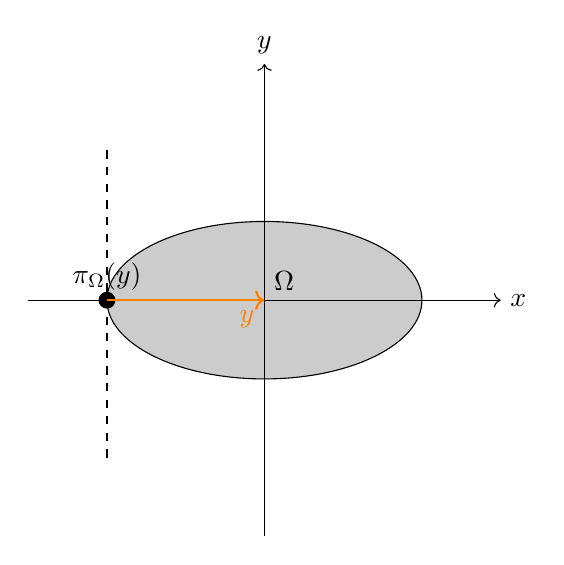
\begin{tikzpicture}[scale=2]
  \draw[fill=gray!40] (0,0) ellipse (1 and 0.5) node[above right] {\(\Omega\)};
  \draw[->] (-1.5,0) -- (1.5,0) node[right] {\(x\)};
  \draw[->] (0,-1.5) -- (0,1.5) node[above] {\(y\)};

  \draw[dashed] (-1,-1) -- (-1,1);
  \draw[fill=black] (-1,0) circle (0.05) node[above] {\(\pi_\Omega(y)\)};
  \draw[->, thick, orange] (-1,0) -- (0,0) node[below left] {\(y\)};
\end{tikzpicture}

\end{lemma}
\begin{proof}{}{}
  La \(g(x) = \frac{1}{2} \norm{x - y}^2\) er strengt-konveks og koersiv (nedadgående uendelig).

  Anta at \(\Omega \neq \emptyset\), lukket og konveks. Da er:
  \[
    \min_{x \in \Omega} g(x) = \min_{x \in \Omega} \frac{1}{2} \norm{x - y}^2
  \]
  et konvekst problem og har en unik løsning.

  \qed
\end{proof}

\begin{proposition}{}{}
  La \(\Omega \subset \R^d\) være ikke-tom, lukket og konveks og \(y \in \R^d\).
  Da er projeksjonen \(\pi_\Omega(y)\) gitt ved det unike punktet som løser betingelsen:
  \[
    \pi_\Omega(y) \in \Omega \quad \text{og} \quad \inner{\pi_\Omega(y) - y, x - \pi_\Omega(y)} \leq 0 \quad \forall x \in \Omega
  \]
  Ekvivalent:
  \[
    \pi_\Omega(y) \in \Omega \quad \text{og} \quad y - \pi_\Omega(y) \in N_\Omega(\pi_\Omega(y))
  \]

\end{proposition}

\begin{proof}{}{}
  Med \(g(x) = \frac{1}{2} \norm{x - y}^2\) har vi at \(\nabla g(x) = x - y\).
  Da er betingelsen:
  \[
    \nabla g(\pi_\Omega(y)) = \pi_\Omega(y) - y \in N_\Omega(\pi_\Omega(y))
  \]
  \qed
\end{proof}

\begin{proposition}{}{}
  Anta at \(\Omega \subset \R^d\) er ikke-tom, lukket og konveks og \(x^\star \in \Omega\).
  \begin{itemize}
    \item Hvis \(x^\star\) er en lokal løsning av (P) da er \(\pi_\Omega(x^\star - \alpha \nabla f(x^\star)) = x^\star\) for alle \(\alpha > 0\) tilstrekkelig liten.
  \end{itemize}
\end{proposition}

\section{Lecture 12 \emph{14. February 2025}}

\begin{proposition}{}{}
  Anta \(\Omega \neq \emptyset\) og konveks, med \(\symbf{x}^\star \in \Omega\).
  \begin{itemize}
    \item Hvis \(\symbf{x}^\star\) er en lokal løsning til (P) da er
          \[
            \pi_{\Omega}(\symbf{x}^\star - \alpha \nabla f(\symbf{x}^\star)) = \symbf{x}^\star \quad \forall \alpha > 0 \tag{\(\ast\)}
          \]
    \item Hvis \(f\) er konveks og differensierbar, og \((\ast)\) holder for en \(\alpha > 0\), da er \(\symbf{x}^\star\) en global løsning til (P).
  \end{itemize}
\end{proposition}

\begin{proof}
  Recall that:
  \begin{align*}
    \symbf{x}^\star = \pi_{\Omega}(\symbf{z}) \iff \symbf{x}^\star \in \Omega \text{ og } \symbf{z} - \symbf{x}^\star \in N_{\Omega}(\symbf{x}^\star)
  \end{align*}
  Thus:
  \begin{align*}
    \symbf{x}^\star & = \pi_{\Omega}(\symbf{x}^\star - \alpha \nabla f(\symbf{x}^\star))                                                     \\
                    & \iff \left(\symbf{x}^\star - \alpha \nabla f(\symbf{x}^\star)\right) - \symbf{x}^\star \in N_{\Omega}(\symbf{x}^\star) \\
                    & \iff -\alpha \nabla f(\symbf{x}^\star) \in N_{\Omega}(\symbf{x}^\star) > 0
  \end{align*}
  \qed
\end{proof}

That is \(\symbf{x}^\star\) is a fixed point of the mapping \(G: \R^d \to \R^d\) defined by:
\[
  G(\symbf{x}) = \pi_{\Omega}(\symbf{x} - \alpha \nabla f(\symbf{x}))
\]
\( \rightarrow \) Fixed point iteration gives the \emph{projected gradient descent method}.


\begin{enumerate}
  \item In step \(k\)
        \begin{align*}
          \symbf{y} \leftarrow \symbf{x}^{(k)} - \alpha \nabla f(\symbf{x}^{(k)}) \\
          \symbf{x} \leftarrow \pi_{\Omega}(\symbf{y})
        \end{align*}
  \item One can show that this method converges if \(\alpha\) is chosen sufficiently small and \(f, \omega\) are \emph{sufficiently nice}.
  \item In practice: Need an effecient way for computing \(\pi_{\Omega}(\symbf{y})\) (the projection onto \(\Omega\)).
        \textbf{E.g.} for \(\Omega = \{ \symbf{x} \in \R^d \mid \symbf{x} \geq \symbf{0} \}\) (the non-negative orthant) we have:
        \[
          \pi_{\Omega}(\symbf{y}) = \max(\symbf{y}, \symbf{0})
        \]
        \begin{center}
          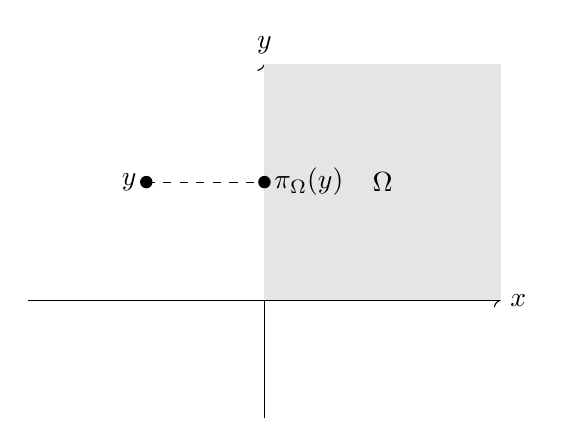
\begin{tikzpicture}[scale=1.5]
            % Axes
            \draw[->] (-2,0) -- (2,0) node[right] {$x$};
            \draw[->] (0,-1) -- (0,2) node[above] {$y$};

            % Quadrant shading
            \fill[gray!20] (0,0) -- (2,0) -- (2,2) -- (0,2) -- cycle;

            % Example point and its projection
            \coordinate (P) at (-1,1);
            \coordinate (Q) at (0,1);

            % Draw projection line
            \draw[dashed] (P) -- (Q);

            % Points
            \fill (P) circle (1.5pt) node[left] {$y$};
            \fill (Q) circle (1.5pt) node[right] {$\pi_\Omega(y)$};

            % Label the region
            \node at (1,1) {$\Omega$};
          \end{tikzpicture}
        \end{center}

\end{enumerate}


\begin{example}{Unit ball}{}
  \[
    \Omega = \mathcal{B}_1(0) = \{ \symbf{x} \in \R^d \mid \norm{\symbf{x}}_2 \leq 1 \}
  \]
  \[
    \pi_{\Omega}(\symbf{y}) = \begin{cases}
      \symbf{y}                            & \text{if } \norm{\symbf{y}}_2 \leq 1 \\
      \frac{\symbf{y}}{\norm{\symbf{y}}_2} & \text{if } \norm{\symbf{y}}_2 > 1
    \end{cases}
  \]
  \begin{tikzpicture}
    % Axes
    \draw[->] (-2,0) -- (2,0) node[right] {$x$};
    \draw[->] (0,-2) -- (0,2) node[above] {$y$};

    % Unit circle
    \draw (0,0) circle (1);

    % Example point and its projection
    \coordinate (P) at (1.5,1.5);
    \coordinate (Q) at (0.707,0.707);

    % Draw projection line
    \draw[dashed] (P) -- (Q);

    % Points
    \fill (P) circle (1.5pt) node[right] {$y$};
    \fill (Q) circle (1.5pt) node[right] {$\pi_\Omega(y)$};
  \end{tikzpicture}
\end{example}

\subsection{Linear constraints}

Consider the set: \(\Omega := \{\symbf{x} : A\symbf{x} = \symbf{b}\}\) where \(A \in \R^{m \times d}\) and \(\symbf{b} \in \R^m\) with \(m < d\).

Now solve \(min_x f(\symbf{x})\) s.t. \(A\symbf{x} = \symbf{b}\).

Let \(\symbf{x} \in \Omega\). Then \(\symbf{p}\) is a feasible direction at \(\symbf{x}\) if :
\begin{align*}
  \symbf{x} + t \symbf{p} \in \Omega \quad \text{for some } t > 0 \\
  \iff A(\symbf{x} + t \symbf{p}) = \symbf{b}                     \\
  \iff A\symbf{x} + t A\symbf{p} = \symbf{b}                      \\
  \iff A\symbf{p} = \symbf{0} \iff p\in \ker(A)
\end{align*}

Thus \(T_{\Omega}(\symbf{x}) = \overline{\ker(A)} = \ker(A)\).

Morover
\begin{align*}
  N_{\Omega}(\symbf{x}) = \{\symbf{q} \in \R^d : \inner{\symbf{q}, \symbf{p}} \leq 0 \quad \forall \symbf{p} \in T_{\Omega}(\symbf{x}) = \ker(A)\} \\
  = \{\symbf{q} \in \R^d : \symbf{q} \cdot \inner{\symbf{q}, \pm \symbf{p}} \leq 0 \quad \forall \symbf{p} \in \ker(A)\}                           \\
  = \{\symbf{q} \in \R^d : \inner{\symbf{q}, \symbf{q}} = 0\}
\end{align*}

\begin{remark}{}{}
  \begin{align*}
    \symbf{p} \in \ker(A) \rightarrow -\symbf{p} \in \ker(A) \\
  \end{align*}
\end{remark}

\begin{remark}{}{}
  We have:
  \begin{align*}
    \left(\ker(A)\right)^\perp = \operatorname{range}(A^T) \rightarrow N_{\Omega}(\symbf{x}) = \operatorname{range}(A^T)
  \end{align*}

  Thus we get the optimality condition:

  \begin{align*}
    + \nabla f(\symbf{x}) \in \operatorname{range}(A^T)
  \end{align*}
  
\end{remark}

\begin{lemma}{}{}
  Assume that \(\symbf{x}^\star\) is a local solution to (P) s.t. \(A \symbf{x} = \symbf{b}\) then there exists a \(\lambda^\star \in \R^m\) s.t.:
  \begin{align*}
    \nabla f(\symbf{x}^\star) + A^T \lambda^\star = 0 \\
    A \symbf{x}^\star = \symbf{b}
  \end{align*}
  Conversly, if \(f\) is convex and \((\symbf{x}^\star, \lambda^\star)\) solves:
  \begin{align*}
    \nabla f(\symbf{x}^\star) = A^T \lambda^\star = 0 \\
    A \symbf{x}^\star = \symbf{b}
  \end{align*}
  then \(\symbf{x}^\star\) is a global solution to (P).
  \emph{Proof?} \(\rightarrow\) optimality conditions. \qed
\end{lemma}

The vector \(\lambda^\star\) is called the \emph{Lagrange multiplier} for \(\symbf{x}^\star\).

\section{Lecture 14 \emph{14. February 2025}}

\begin{definition}{Slater's Condition}{slater_condition}
  For a convex problem with inequality constraints
  \[
    c_i(x) \le 0,\quad i=1,2,\dots,m,
  \]
  Slater's condition holds if there exists an \(x\) such that
  \[
    c_i(x) < 0 \quad \text{for all } i.
  \]
\end{definition}

\begin{remark}{Intuition}{}
  This condition guarantees that the feasible region has a nonempty interior.

  In other words, the constraints are not all 'tight' at every point, which helps secure strong duality and the existence of Lagrange multipliers.
\end{remark}

\begin{theorem}{KKT conditions}{kkt}

  \medskip

  \begin{itemize}
    \item \(A_i\) are the active constraints/indices at \(x\)
    \item \(C\) is the matrix of equality constraints.
    \item \(p\) is the direction of descent.
    \item \(x\) is the current point (feasible).
    \item \(T_{\Omega}(x)\) is the tangent cone at \(x\).
    \item \(c_i(x)\) is the value of the \(i\)-th constraint at \(x\).
    \item \(Ax\) is the value of the equality constraints at \(x\).
    \item \(b\) is the vector of equality constraints.
  \end{itemize}
  \begin{align*}
    \mathcal{A}_1(x)            & := \{i \in \mathcal{I} \mid c_i(x) = 0\},                     \\
    \mathcal{A}_2(x)            & := \{1 \leq i \leq m \mid (Ax)_i = b_i\} \tag{Active indices} \\
    \text{Active indices at } x & \in \Omega                                                    \\
  \end{align*}

  Assume that \emph{Slater's constraint} holds. Then, the following statements are equivalent:

  \begin{align*}
    p\in T_{\Omega}(x) & \Longleftrightarrow
    \begin{cases}
      \inner{\nabla c_i(x), p} \geq 0, & i \in \mathcal{A}_1(x) \\
      (Ax)_i \geq 0,                   & i \in \mathcal{A}_2(x) \\
      Cp = 0,                          &                        \\
    \end{cases}
  \end{align*}

\end{theorem}


\begin{lemma}{Farka's Lemma}{farkas_lemma}
  Let \(A \in \mathbb{R}^{m \times n}\) and \(c \in \mathbb{R}^n\). Then, exactly one of the following statements is true:
  \begin{enumerate}
    \item[] \((1)\) There exists an \(x \in \mathbb{R}^n\) such that \(Ax \preceq 0\) and \(c^T x < 0\).
    \item[] \((2)\) There exists a \(y \in \mathbb{R}^m\) such that \(A^T y + c = 0\) and \(y \succeq 0\).
  \end{enumerate}
\end{lemma}

\begin{proof}
  \begin{enumerate}
    \item[] Assume that \((1)\) holds. Then \(Ax = b\) and \(x \ge 0\). If there exists a \(y\) such that \(y^T A \ge 0\), then
          \[
            y^T b = y^T Ax = (y^T A)x \ge 0,
          \]
          which contradicts \(y^T b < 0\).
    \item[] Assume that \((1)\) does not hold. We want to show that \((2)\) holds.

          Let
          \[
            K = \{Ax \mid x \ge 0\}.
          \]
          Since \((1)\) does not hold, \(b \notin K\). Since \(K\) is a closed convex cone, by the separating hyperplane theorem, there exists a \(y \in \mathbb{R}^m\) such that
          \[
            y^T b < y^T z \quad \text{for all } z \in K.
          \]
          Since \(0 \in K\), we have \(y^T b < 0\).

          Now, for any \(x \ge 0\), we have \(Ax \in K\), so \(y^T b < y^T Ax\).

          Let \(x = e_i\), where \(e_i\) is the \(i\)-th standard basis vector. Then \(x \ge 0\), and
          \[
            y^T A e_i = (y^T A)_i > 0.
          \]
          Thus \(y^T A \ge 0\).
  \end{enumerate}

  \begin{center}
    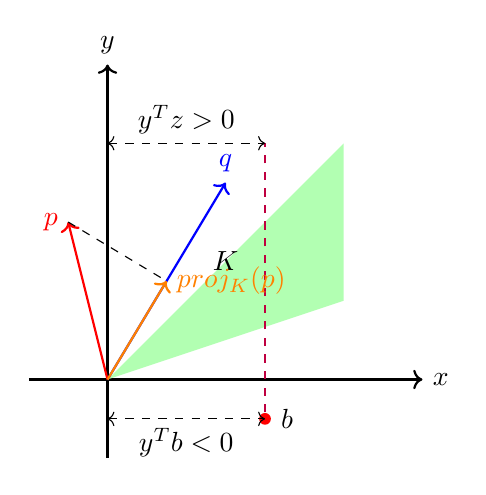
\begin{tikzpicture}
      \draw[->, thick] (-1, 0) -- (4, 0) node[right] {$x$};
      \draw[->, thick] (0, -1) -- (0, 4) node[above] {$y$};

      \fill[green!30] (0, 0) -- (3, 1) -- (3, 3) -- cycle;
      \node at (1.5, 1.5) {$K$};

      \node[circle, fill=red, inner sep=1.5pt, label=right:$b$] (b) at (2, -0.5) {};

      \draw[dashed, purple] (b) -- (2, 3);
      \draw[<->, dashed, black] (0, -0.5) -- (2, -0.5) node[midway, below, black] {$y^Tb < 0$};
      \draw[<->, dashed, black] (0, 3) -- (2, 3) node[midway, above, black] {$y^Tz > 0$};

      % Adding new vectors
      \draw[->, thick, blue] (0, 0) -- (1.5, 2.5) node[above] {$q$};
      \draw[->, thick, red] (0, 0) -- (-0.5, 2) node[left] {$p$};
      \draw[->, thick, orange] (0, 0) -- (0.75, 1.25) node[right] {$proj_K(p)$};
      \draw[dashed] (-0.5, 2) -- (0.75, 1.25);
    \end{tikzpicture}
  \end{center}

  The figure illustrates the geometric interpretation of Farkas' Lemma. The green region $K$ represents the cone of feasible points $\{Ax \mid x \ge 0\}$. The point $b$ (in red) lies outside this cone. The purple dashed line represents the separating hyperplane, which separates $b$ from $K$. Vector $p$ (in red) is projected onto the cone $K$, resulting in $proj_K(p)$ (in orange). Vector $q$ (in blue) lies inside the cone $K$. The black dashed lines show that the inner product $y^Tb$ is negative, while the inner product $y^Tz$ is positive for points $z$ in the cone $K$.

\end{proof}


\begin{theorem}{KKT conditions}{kkt_conditions}
  Assume \(c_i, i \in \mathcal{I}\) are concave in \(\mathcal{C}^1\),
  \(A\in \mathbb{R}^{m \times d}, b \in \mathbb{R}^m\) and \(C\in \mathbb{R}^{l \times d}\) and that \(f:\mathbb{R}^d \to \mathbb{R}\) is \(\mathcal{C}^1\). Assume that \emph{Slater's condition} holds.

  If \(x^\star\) is a local minimum of \(\min_x f(x)\) s.t.
  \[
    \begin{cases}
      c_i(x) \geq 0, & \forall i \in \mathcal{I} \\
      Ax \geq b,     &                           \\
      Cx = b,        &
    \end{cases}
  \]
  then there exists a \emph{Lagrange multipliers} \(\lambda^\star, \mu^\star\) with \(v \in \R^e\) s.t. the \emph{KKT conditions} hold:

  Then, the following statements are equivalent:
  \begin{align}
    \nabla f(x^\star) = \sum_{i\in \mathcal{I}} \lambda_i^\star \nabla c_i(x^\star) + A^T \mu^\star + C^T v^\star \\
    \begin{cases}
      c_i(x^\star) \geq 0, & \forall i \in \mathcal{I} \\
      Ax^\star \geq b,     &                           \\
      Cx^\star = e,        &                           \\
    \end{cases} \tag{Feasibility}                                                              \\
    \begin{cases}
      \lambda_i^\star \geq 0, & \forall i \in \mathcal{I} \\
      \mu_j^\star \in \geq 0, & \forall j \in \mathcal{J} \\
    \end{cases} \tag{Dual feasibility}                                                           \\
    \begin{cases}
      \lambda_i^\star c_i(x^\star) = 0, & \forall i \in \mathcal{I} \\
      \mu_j^\star C_j^T = 0,            & \forall j \in \mathcal{J} \\
    \end{cases} \tag{Complementary slackness}                                                 \\
    \begin{cases}
      \lambda_i^\star c_i(x^\star) = 0,      & \forall i \in \mathcal{I} \\
      \inner{\mu_j^\star, Ax^\star - b} = 0, & \forall j \in \mathcal{J} \\
    \end{cases} \tag{Complementary slackness}
  \end{align}
\end{theorem}

\begin{proof}{}{}
  We have the optimality condition:
  \[
    \inner{\nabla f(x^\star), p} \geq 0 \, \forall p \in T_{\Omega}(x^\star)
  \]
  \medskip
  \begin{align*}
    p \in T_{\Omega}(x^\star) \iff
    \begin{cases}
      \inner{\nabla c_i (x^\star), p }\geq 0 & \forall i \in \mathcal{A}_1(x^\star)                         \\
      \text{or: there does not exist any } p \in \R^d \text{ such that:} & \\
      \begin{cases}
        \inner{\nabla c_i (x^\star), p }\geq 0 & \forall i \in \mathcal{A}_1(x^\star) \\
        \inner{A_i^T , p }\geq 0               & \forall i \in \mathcal{A}_2(x^\star) \\
        \inner{ (C_i )^T, p } = 0              & \forall 1 \leq i \leq l              \\
        \inner{\nabla f (x^\star), p } < 0     & 
      \end{cases}                             \\
      (Ap)_i \geq 0 & \forall i \in \mathcal{A}_2(x^\star)                                                      \\
      Cp = 0        &
    \end{cases}
  \end{align*}

  The second alternative is Farka's Lemma does not hold \(\implies\) The first holds.

  \begin{align*}
    \nabla f(x^\star) & = \sum_{i\in \mathcal{A}_1(x^\star)} \lambda_i^\star \nabla c_i(x^\star) + \sum_{i \in \mathcal{A}_2(x^\star)} \mu_i^\star A_i^T + \sum_{i=1}^l v_i^\star C_i^T \\
  \end{align*}

  For some  \(\lambda_i^\star \geq 0, \mu_i^\star \geq 0, v_i^\star \in \R\).

  Now define: \(\lambda_i^\star = 0 \) for \(i \notin \mathcal{A}_1(x^\star)\) and \(\mu_i^\star = 0\) for \(i \notin \mathcal{A}_2(x^\star)\).

  Then we have:
  \begin{align*}
    \nabla f(x^\star) & = \sum_{i\in \mathcal{I}} \lambda_i^\star \nabla c_i(x^\star) + \sum_{1 \leq i \leq m} \mu_i^\star A_i^T + \sum_{1 \leq i \leq l} v_i^\star C_i^T = \text{(1)} \\
  \end{align*}
  \qed
\end{proof}

\begin{definition}{The Lagrangian of a problem}{lagrangian}
  The Lagrangian of a problem is the function \(\mathcal{L}: \mathbb{R}^d \times \mathbb{R}^m \times \mathbb{R}^l \times \mathbb{R}^e \to \mathbb{R}\) defined as:
  \begin{align*}
    \mathcal{L}(x, \lambda, \mu, v) &= f(x) + \sum_{i\in \mathcal{I}} \lambda_i c_i(x) + \sum_{1 \leq i \leq m} \mu_i (Ax - b)_i + \sum_{1 \leq i \leq l} v_i (Cx - b)_i \\
    &= f(x) - \sum_{i \in \mathcal{I}} \lambda_i c_i(x) - \inner{\mu, Ax - b} - \inner{v, Cx - e}\footnote{\( (1) \iff \nabla_x \mathcal{L}(x, \lambda, \mu, v) = 0\)}
  \end{align*}

\end{definition}




\printbibliography
\printglossary
\printglossary[type=\acronymtype]

\end{document}
